\documentclass[a4j]{jarticle}
\usepackage[dvipdfmx]{graphicx}
\usepackage{amssymb}
\usepackage{subfigure}

\begin{document}

\begin{table}[t]
\begin{center}
{\Large LTE 環境における応答遅延特性の時系列モデリングを用いた分析}\\
山本 航平\\
令和 2 年 3 月 25 日
\end{center}
\vspace{1cm}
\begin{tabular}{l}
\hspace{0.5cm}{\large -進捗報告-}\\
・原稿執筆を行っております\\
・ARMA-GARCH モデルを用いたクラスタリングを行いました\\
\end{tabular}
\end{table}

\section{計測実験の設定}
本報告では図 \ref{exp} に示す構成で計測実験を行った.
モニタリングシステムにおける無線端末としては LTE モジュールとして Quectel 社製 EC21-J を搭載した Raspberry Pi を用いた.
また,LTE 回線としては IIJ モバイル社のサービスタイプ D 定額プランライト(いちねん プリペイド)を用いた.
IIJ モバイル社は他の通信事業者から通信回線を借り受け,サービスを提供している MVNO(Mobile Virtual Network Operator)であり,サービスタイプ D では NTT ドコモ社の回線を使用している.
月あたり通信量が 3GB を超過すると通信速度が 256kbps に制限されるが,本実験中には速度制限は課されなかった.

クラウドサーバとしては本計測を行うにあたり契約した一台の AWS サーバを用い,大阪大学敷地内の研究室に設置した Raspberry Pi から ping を用いて応答遅延を計測した.
自動的に計測データを取得できるよう,Raspberry Pi 上で動作する Raspbian において計測用のスクリプトを用いることで, 15 秒毎に時刻を取得し,続けて ping (パケットサイズ 60 バイト, ICMP ECHO メッセージ,パケット数 1 )を実行した.
計測時刻,ping の出力をログデータとして取り出し,分析を行った.
また,日時が応答遅延に与える影響を調べるため,様々な時間帯で計測を行った.
計測は 2/29(土)から 3/27(金)までの四週間に渡って行った.
\begin{figure}[tb]
\centering
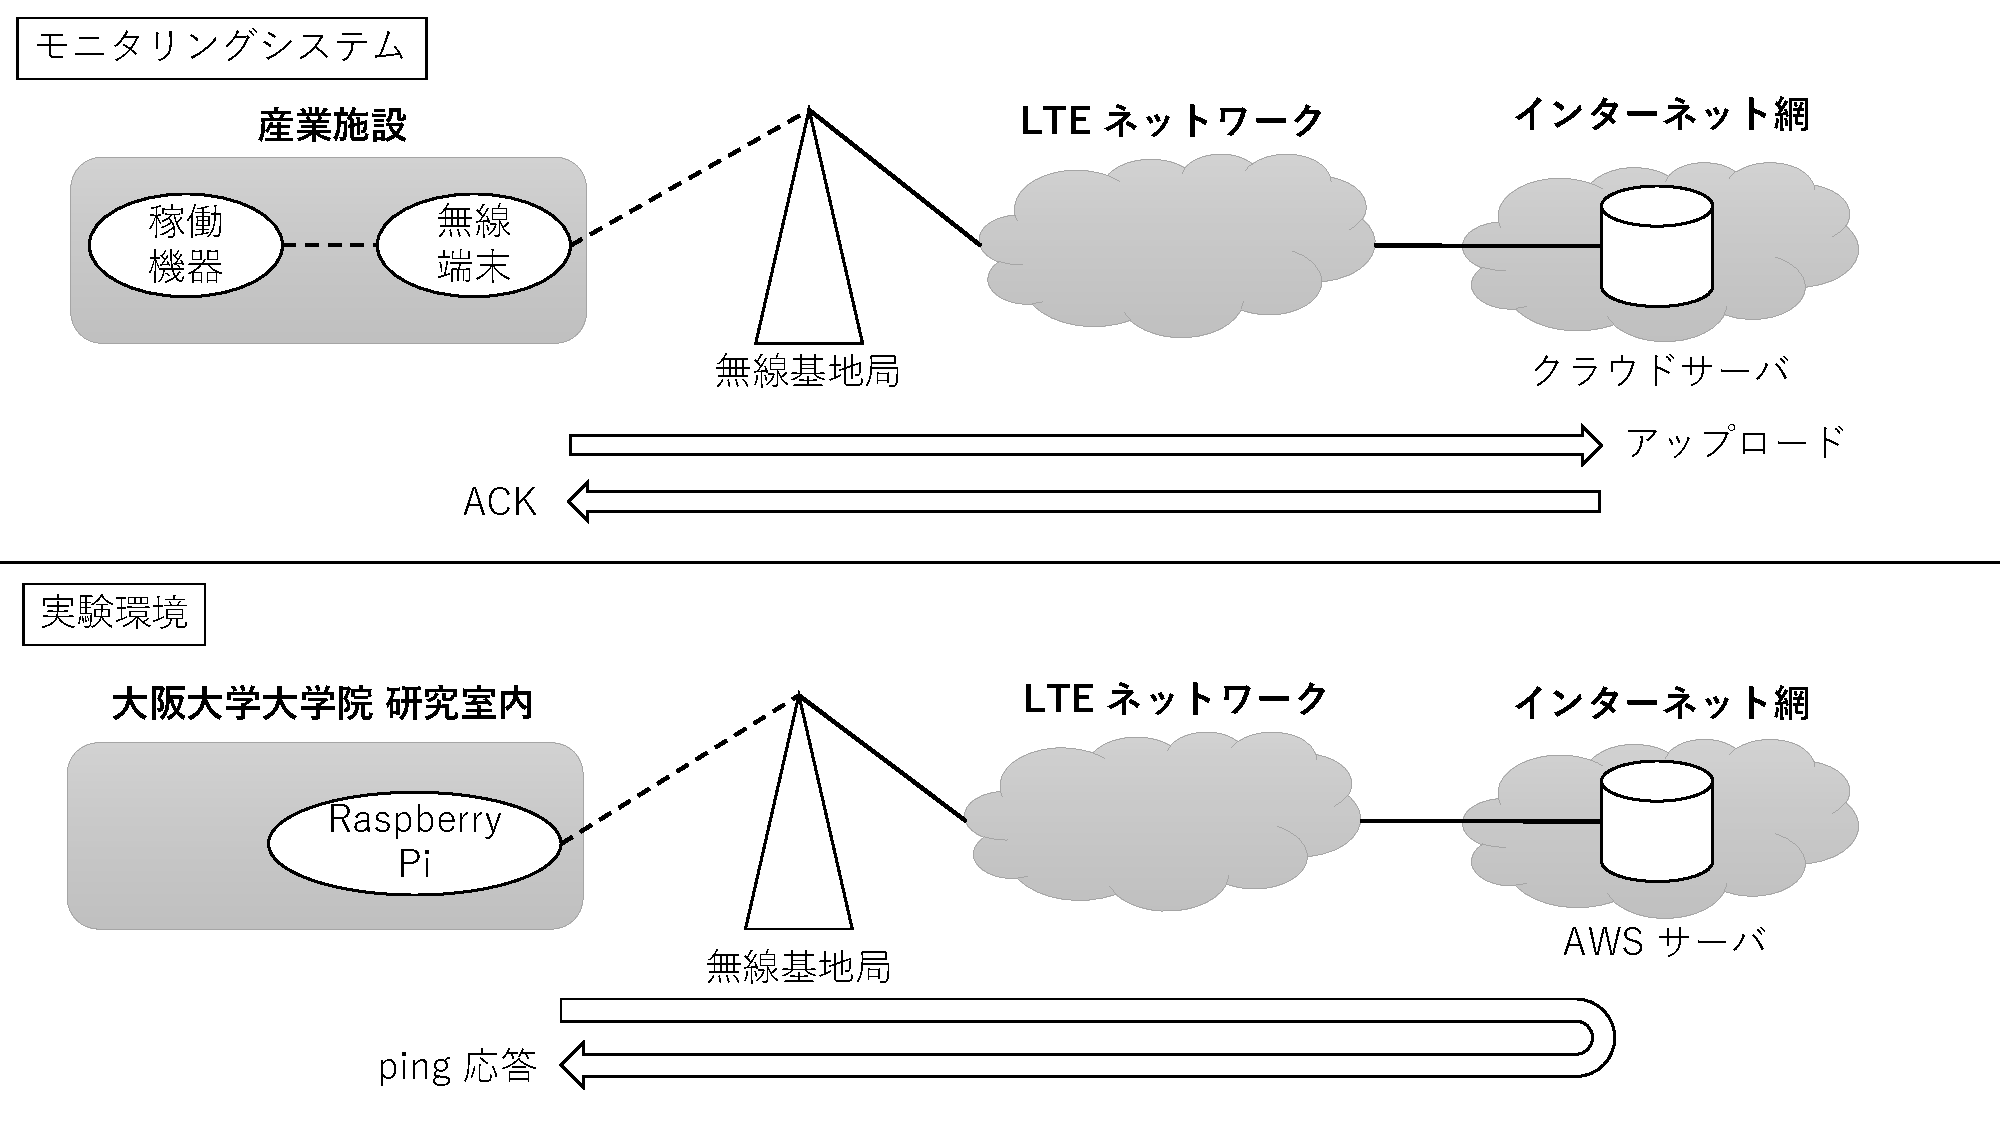
\includegraphics[width=7.5cm]{../figure/experiment.pdf}
\caption{モニタリングシステムと実験環境の対応図}
\label{exp}
\end{figure}

\section{時系列モデルによる回帰}
本報告では,時系列モデルとして式 (\ref{garch1}) と式 (\ref{garch2}) で表される ARMA-GARCH(Autoregressive Moving Average - Generalized Autoregressive Conditional Heteroscedasticity)モデルを用いる.
\begin{equation}
y_t = \sum_{i=1}^p a_i y_{t-i} + \sum_{i=1}^q b_i \varepsilon_{t-i} + c + \varepsilon_{t} \hspace{1.5cm}\varepsilon_t \sim N(0,h_t) \hspace{0.5cm} i.i.d
\label{garch1}
\end{equation}
\begin{equation}
\displaystyle h_{t} = \omega + \sum_{i=1}^{r}\alpha_i\varepsilon_{t-i}^2 + \sum_{i=1}^{s}\beta_ih_{t-i}
\label{garch2}
\end{equation}
本報告では,各一時間の計測実験において Raspberry Pi が AWS サーバから受け取る ping の応答遅延の実測値を計測時刻順に $y_1$,$y_2$,...,$y_N$ と表す.
式 (\ref{garch1}) において,$c$ は定数項,$\varepsilon_t$ はノイズ項であり平均 0 分散 $h_t$ の正規分布に従いそれらは互いに独立であるとし,時刻 $t$ における実測値 $y_t$ は,過去の $p$ 時点前までの実測値の線形和と $q$ 時点前までのノイズ項の加重和と自身のノイズ項によって表される.
また,式 (\ref{garch2}) において,$\omega$ は定数項であり,時刻 $t$ におけるノイズ項が従う正規分布の分散 $h_t$ は,過去の $r$ 時点前までのノイズ項の線形和と $s$ 時点前までのノイズ項が従う正規分布の分散の加重和によって表される.

各パラメータのパラメータ数 $(p,q,r,s)$ は次数と呼ばれ,精度の良い回帰を行うためには対象とする時系列データに応じてこの次数を適切に定める必要がある.
しかしながら,計測データのクラスタリングによる分類のためには異なる曜日や時間帯での計測によって得られた時系列データに対して次数を統一して回帰しなければならない.
そこで,本報告では,まず,各計測データに対し ARMA-GARCH モデルの次数を変えながら適用し,AIC(赤池情報量規準)によってその妥当性を評価することで,各時系列データにとって適切な次数を求める.
ここで,AIC は式(\ref{aic})で定められる指標である.
高すぎる次元での回帰による過適合の問題を考慮し,時系列モデルによる回帰のよさを評価する第 1 項とパラメータの少なさを評価する第 2 項を組み合わせている.
AICが小さいほどよいモデルとされている.
\begin{equation}
AIC = -2 *(対数尤度)+2 *(パラメータ数)
\label{aic}
\end{equation}
次に,各時系列データ間で AIC による最適次数を比較し,その最大のものを用いることとする.
次数の探索範囲は $0 \le p \le 2$,$0 \le q \le 2$,$r = 1$,$0 \le s \le 1$ とした.

各時系列データをその最適次数ごとに数えると表 \ref{count_norm} となり,統一する次数は $(p,q,r,s) = (2,2,1,1)$ となった.
この次数での ARMA-GARCH モデルによる回帰結果の一部を \ref{norm-reg} に示す.

また,応答遅延の変動に注目し,応答遅延の実測値の差分系列 $\{\Delta y_t | y_t - y_{t-1}\}$ に対しても同様にモデルの適用を行った.
この各差分系列の時系列データをその最適次数ごとに数えると表 \ref{count_diff} となり,統一する次数は $(p,q,r,s) = (2,2,1,1)$ となった.
この次数での 差分系列に対する ARMA-GARCH モデルでの回帰結果の一部を図 \ref{diff-reg} に示す.

\begin{table}[h]
\centering
\caption{最適次数と対応する時系列データの数}
\label{count_norm}
\begin{tabular}{|l|l|}
\hline
次数 $(p,q,r,s)$ & 個数\\
\hline
(0,0,1,0) & 9\\
\hline
(0,0,1,1) & 6\\
\hline
(0,1,1,0) & 11\\
\hline
(0,1,1,1) & 4\\
\hline
(0,2,1,0) & 5\\
\hline
(0,2,1,1) & 3\\
\hline
(1,0,1,0) & 3\\
\hline
(1,0,1,1) & 3\\
\hline
(1,1,1,0) & 4\\
\hline
(1,1,1,1) & 1\\
\hline
(1,2,1,0) & 6\\
\hline
(1,2,1,1) & 8\\
\hline
(2,0,1,0) & 4\\
\hline
(2,0,1,1) & 3\\
\hline
(2,1,1,0) & 3\\
\hline
(2,1,1,1) & 1\\
\hline
(2,2,1,0) & 21\\
\hline
(2,2,1,1) & 11\\
\hline
\end{tabular}
\end{table}

\begin{table}[h]
\centering
\caption{最適次数と対応する差分系列の時系列データの数}
\label{count_diff}
\begin{tabular}{|l|l|}
\hline
次数 $(p,q,r,s)$ & 個数\\
\hline
(0,0,1,0) & 0\\
\hline
(0,0,1,1) & 0\\
\hline
(0,1,1,0) & 11\\
\hline
(0,1,1,1) & 4\\
\hline
(0,2,1,0) & 7\\
\hline
(0,2,1,1) & 3\\
\hline
(1,0,1,0) & 0\\
\hline
(1,0,1,1) & 0\\
\hline
(1,1,1,0) & 4\\
\hline
(1,1,1,1) & 2\\
\hline
(1,2,1,0) & 21\\
\hline
(1,2,1,1) & 10\\
\hline
(2,0,1,0) & 0\\
\hline
(2,0,1,1) & 0\\
\hline
(2,1,1,0) & 2\\
\hline
(2,1,1,1) & 0\\
\hline
(2,2,1,0) & 19\\
\hline
(2,2,1,1) & 23\\
\hline
\end{tabular}
\end{table}

\begin{figure}[tb]
\centering
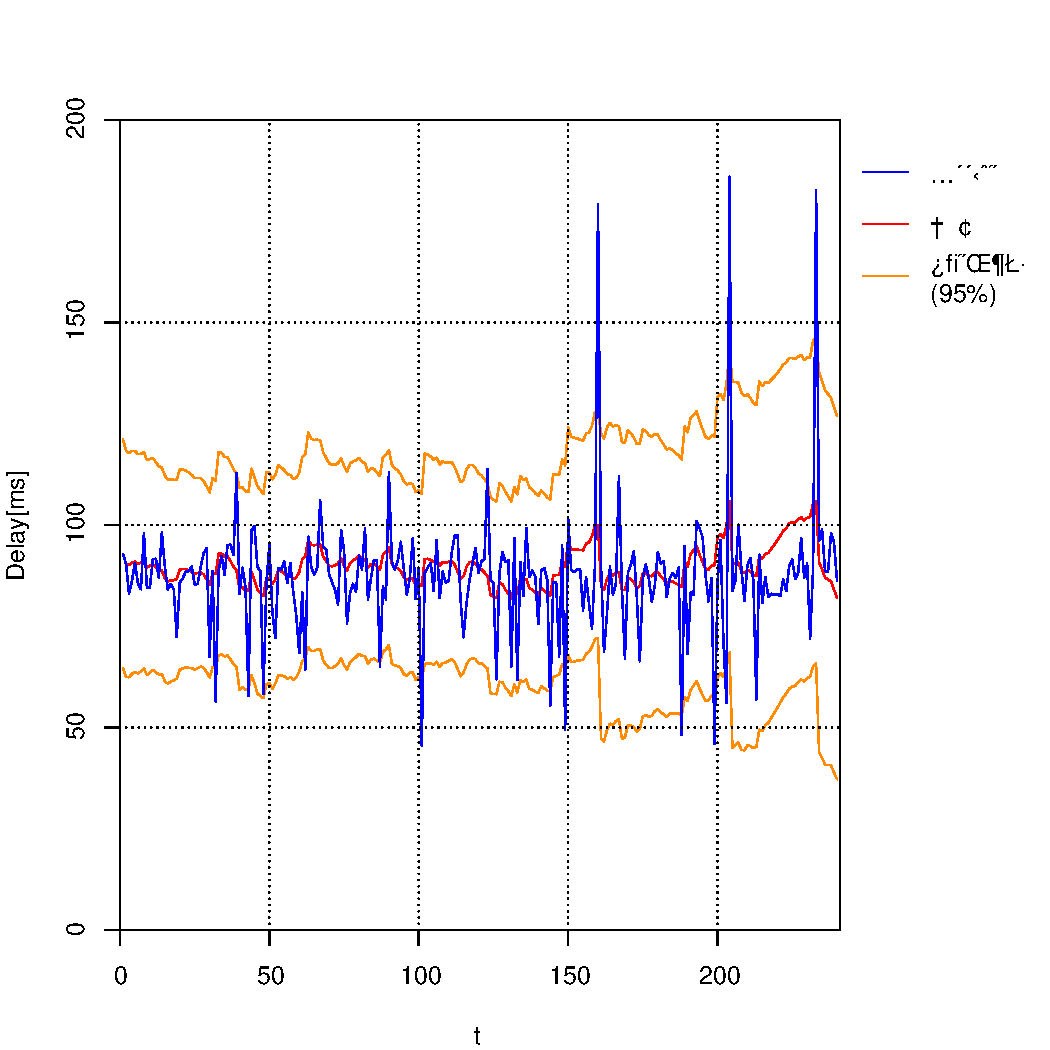
\includegraphics[width=10cm]{../figure/0301_12-plot}
\caption{実測値に対する次数 (2,2,1,1) のARMA-GARCH モデルでの回帰結果}
\label{norm-reg}
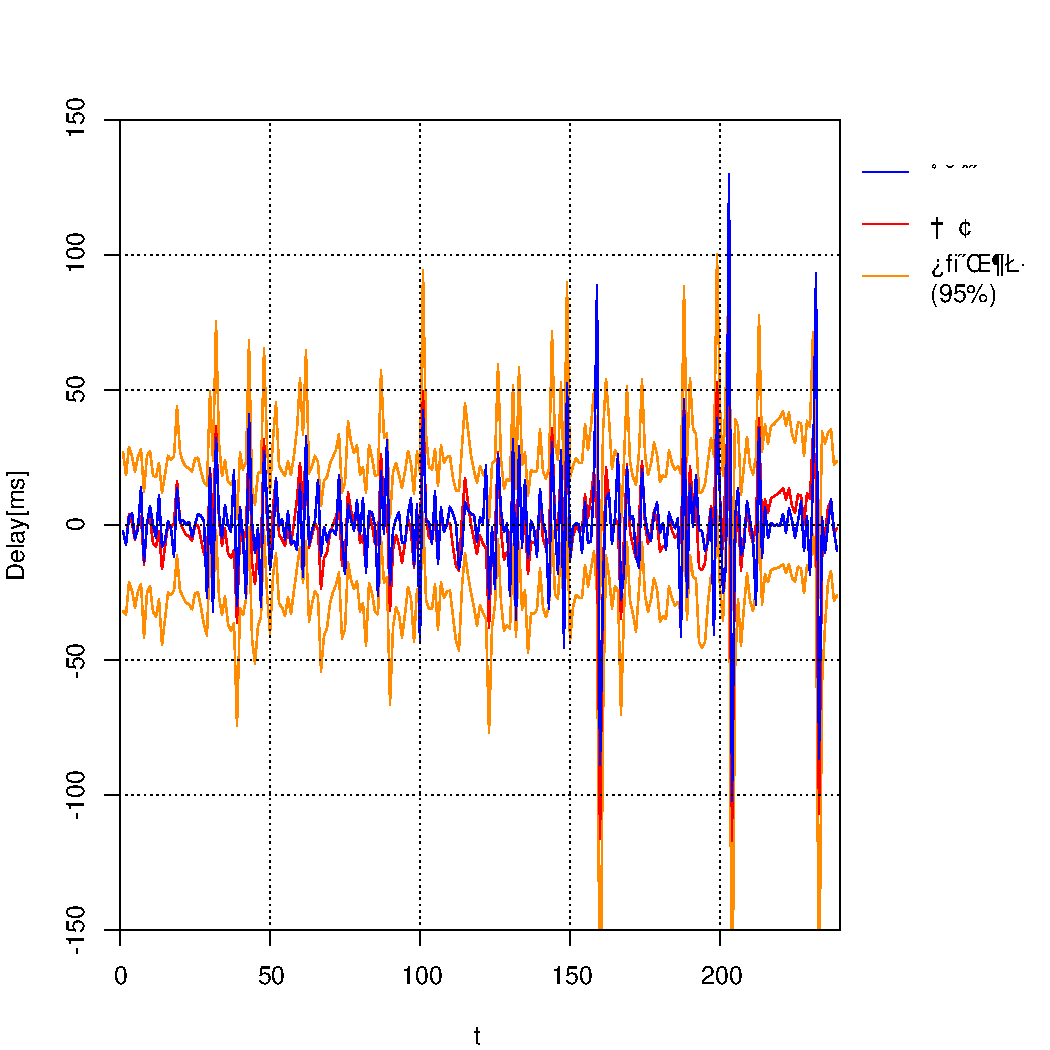
\includegraphics[width=10cm]{../figure/0301_12-plot-diff}
\caption{変動値に対する次数 (2,2,1,1) のARMA-GARCH モデルでの回帰結果}
\label{diff-reg}
\end{figure}


次数 (2,2,1,1) の ARMA-GARCH モデルでは冗長なパラメータが全体に占める割合が小さくなるといえない.
例えば,最適次数 (1,0,1,0) の差分処理なしのある時系列データに対して次数 (2,2,1,1) とした場合の各パラメータは表 \ref{par} のようになっており,冗長なパラメータ $a_2$ は最適な次数に含まれる $a_1$ と比べて小さくなかった.

\begin{table}[h]
\centering
\caption{最適次数(1,0,1,0) に対する次数(2,2,1,1) のモデル適用時の各パラメータ}
\label{par}
\begin{tabular}{|l|l|l|l|l|l|l|l|}
\hline
$c$&$a_1$&$a_2$&$b_1$&$b_2$&$\omega$&$\alpha_1$&$\beta_1$\\
\hline
20.82&0.330&0.385&-0.388&-0.388&0.0001&0.001&0.999\\
\hline
\end{tabular}
\end{table}

\section{クラスタリングによる分類}
 ARMA-GARCH モデルを実測値データもしくは変動値データに対して適用した結果定まるパラメータ $W$ をもとにクラスタリングを行い,時間帯や場所ごとの ping 応答遅延特性を分析する.
また, $W$ は,実測値データと差分系列データともに
$$W = [c, a_1, a_2, b_1, b_2, \omega, \alpha_1, \beta_1] $$
で与えられる.

クラスタリング手法には様々なものが存在するが,本報告では階層クラスタリングと非階層クラスタリングを用いる.
階層クラスタリングは,クラスタリング対象の各要素間の近似度(距離)に基づき,最も近い要素同士を集めてクラスタを形成する手法である.
また,クラスタ数を指定した数と一致させる場合,クラスタ間距離に基づき最も近いものの間でクラスタ融合が起こる.
本研究では,距離関数に以下の三つを用いる(要素 $W_i = [w_{i1},w_{i2},...,w_{in}] と W_j = [w_{j1},w_{j2},...,w_{jn}]$)
\begin{itemize}
\item ユークリッド距離 : $\sqrt{( W_i - W_j )^2}$
\item マンハッタン距離 : $\sum^n_{k=1} |w_{ik}-w_{jk}| $
\item キャンベラ距離 : $\sum^n_{k=1}\frac{|w_{ik}-w_{jk}|}{|w_{ik}|+|w_{jk}|} $
\end{itemize}
また,クラスタ融合手法として以下の三つを用いる.
\begin{itemize}
\item 重心法 : クラスタ間の重心距離が最小のクラスタ同士を融合する
\item 最近傍法 : クラスタ間の要素対のうち,最も近い要素間をクラスタ間距離として,クラスタ間距離が最も小さいクラスタ同士を融合する
\item ウォード法 : 融合後のクラスタ内分散から融合前の二つのクラスタ内分散の差を最小とするという基準でクラスタを融合する
\end{itemize}

階層クラスタリングはこの距離関数とクラスタ融合手法の各組合せ 9 通りを検証する.

非階層的クラスタリングには k 平均法を用いる.
これは,各要素を k 個のクラスタ中心のうち最も近いクラスタ中心のクラスタに分類し,形成させたクラスタの中心を求め,k 個のクラスタ中心を更新する,という処理をクラスタ中心が移動しなくなるまで繰り返すことで行われるクラスタリングである.

実測値の時系列データおよび変動値の時系列データのそれぞれに対し,これらの階層クラスタリングと非階層クラスタリングを用いて,時系列モデルのパラメータに基づいたクラスタリングを行う.

また,クラスタ数は 6,7,9,12,15 とした.

以下その結果を図 \ref{cluster1} から図 \ref{cluster2} に示す.
このそれぞれは,該当するクラスタリングによって分類された計測データを,計測した時間帯もしくは曜日ごとに色分けした積み上げ棒グラフである.縦軸は各クラスタ内の個数に対する割合であり,上部に各クラスタに属する計測データの個数を示している.

さらに標準化を行ったパラメータの主成分でのクラスタリングも行う.
これは,パラメータ間で大きさや分散が異なること,次元数が多いことによりクラスタリングの精度が低下する可能性を考え,その対処として行った.
その結果を図 \ref{cluster3} から図 \ref{cluster4} に示す.
実測値データを主成分分析した結果の累積寄与率は表 \ref{norm-comp-summary} となっており,累積寄与率が 70\% を超えた第三主成分までを用いてクラスタリングを行う.
この時の各主成分の負荷量は表 \ref{norm-comp-loading} となっていた.
変動値データに関しては,主成分分析における累積寄与率は表 \ref{diff-comp-summary} となっており,累積寄与率が 70\% を超えた第三主成分までを用いてクラスタリングを行う.
この時の各主成分の負荷量は表 \ref{diff-comp-loading} となっていた.

\begin{table}[tb]
\centering
\caption{実測値データの主成分分析における累積寄与率}
\label{norm-comp-summary}
\begin{tabular}{|l|l|l|l|}
\hline
第一主成分&第二主成分&第三主成分&第四主成分\\
\hline
44.9\%&67.6\%&85.9\%&96.8\%\\
\hline
\end{tabular}
\end{table}

\begin{table}[tb]
\centering
\caption{実測値データの第三主成分までのそれぞれのおける負荷量}
\label{norm-comp-loading}
\begin{tabular}{|l|l|l|l|}
\hline
&第第一主成分&第二主成分&第三主成分\\
$c$&0.513&0.154& \\
$a_1$&-0.411&-0.179&-0.464\\
$a_2$&-0.403& &0.520\\
$b_1$&0.415&0.191&0.449\\
$b_2$&0.392& &-0.537\\
$\omega$&-0.141&0.578& \\
$\alpha_1$&-0.140&0.394&-0.136\\
$\beta_1$&0.201&-0.644& \\
\hline
\end{tabular}
\end{table}

\begin{table}[tb]
\centering
\caption{変動値データの主成分分析における累積寄与率}
\label{diff-comp-summary}
\begin{tabular}{|l|l|l|l|}
\hline
第一主成分&第二主成分&第三主成分&第四主成分\\
\hline
37.4\%&54.8\%&70.0\%&82.6\%\\
\hline
\end{tabular}
\end{table}

\begin{table}[tb]
\centering
\caption{変動値データの第三主成分までのそれぞれのおける負荷量}
\label{diff-comp-loading}
\begin{tabular}{|l|l|l|l|}
\hline
&第第一主成分&第二主成分&第三主成分\\
$c$& &0.317&0.591\\
$a_1$&-0.566&-0.104& \\
$a_2$& &-0.277&-0.518\\
$b_1$&-0.568& & \\
$b_2$&0.570& & \\
$\omega$&0.113&0.595&-0.416\\
$\alpha_1$& &0.177&-0.457\\
$\beta_1$& &-0.638& \\
\hline
\end{tabular}
\end{table}

\begin{figure}[tb]
\begin{center}
\subfigure[クラスタ数 6 : 時間帯]{
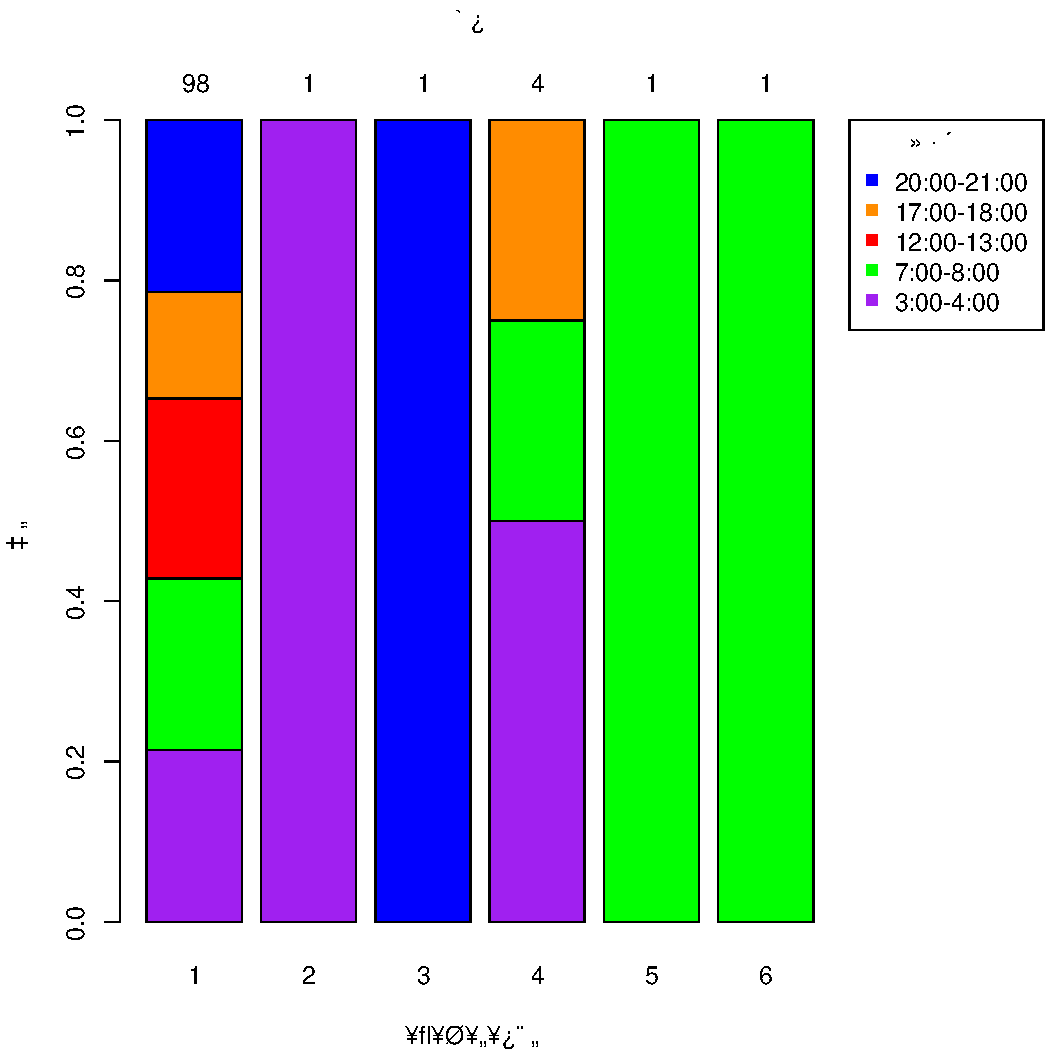
\includegraphics[height=4cm,width=6cm]{../figure/norm-eucl-cent-6-timezone.pdf}
}~
\subfigure[クラスタ数 6 : 曜日]{
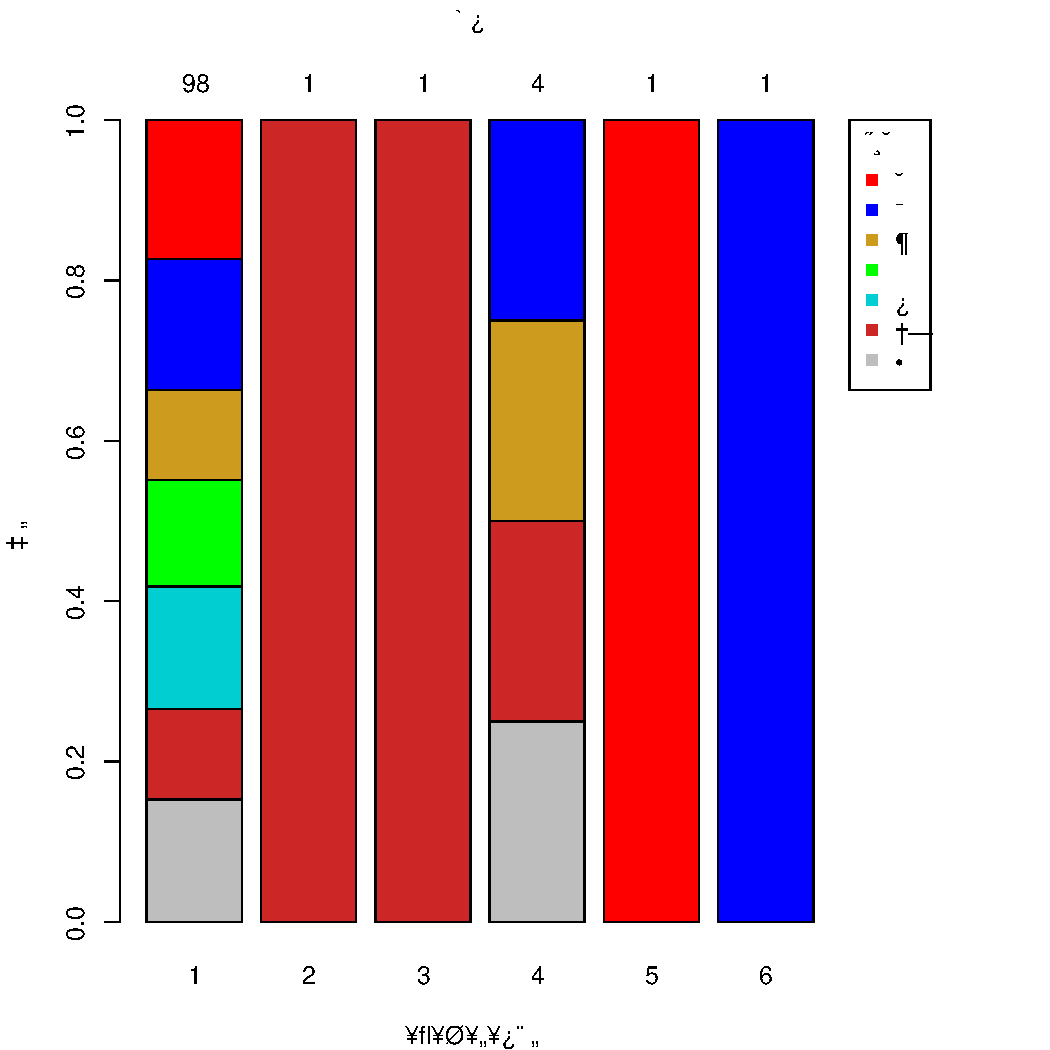
\includegraphics[height=4cm,width=6cm]{../figure/norm-eucl-cent-6-day.pdf}
}\\
\subfigure[クラスタ数 7 : 時間帯]{
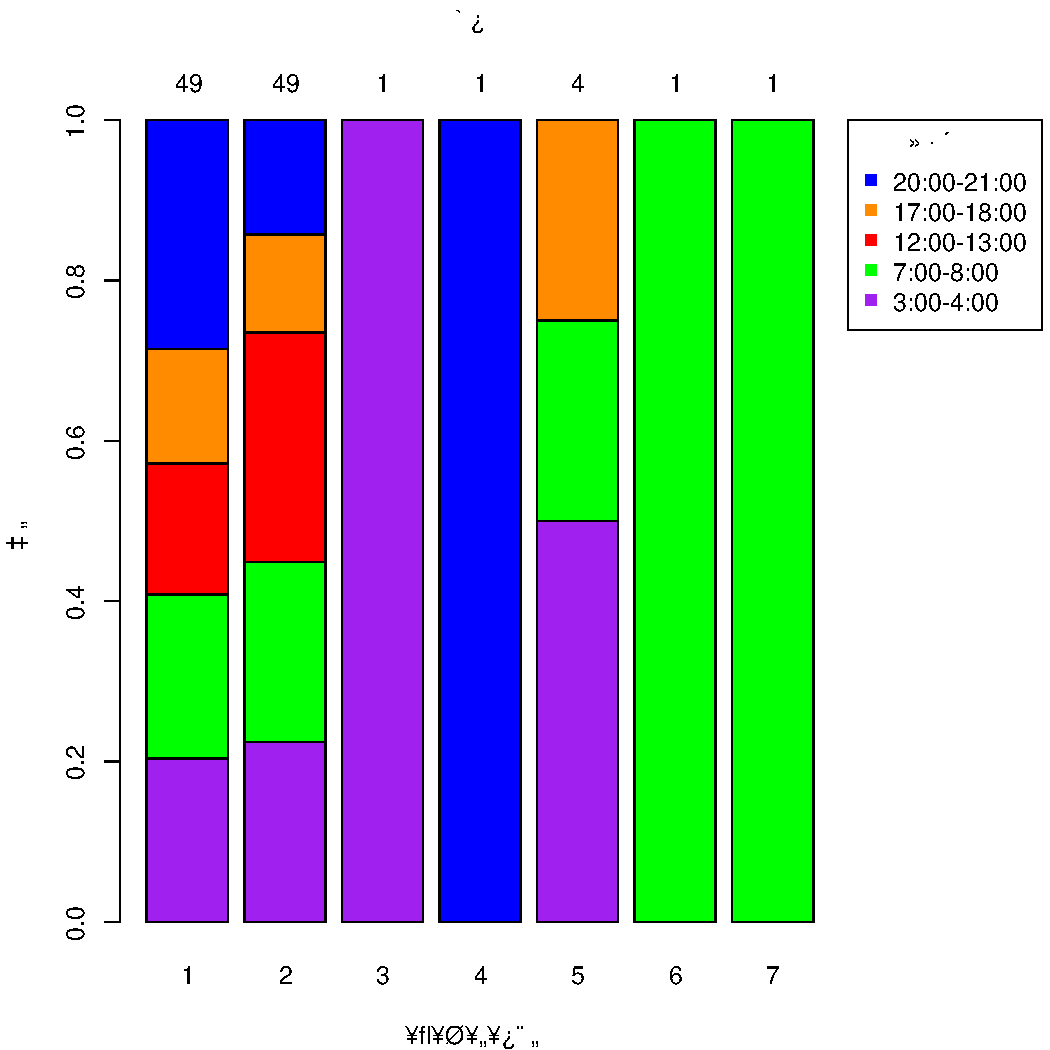
\includegraphics[height=4cm,width=6cm]{../figure/norm-eucl-cent-7-timezone.pdf}
}~
\subfigure[クラスタ数 7 : 曜日]{
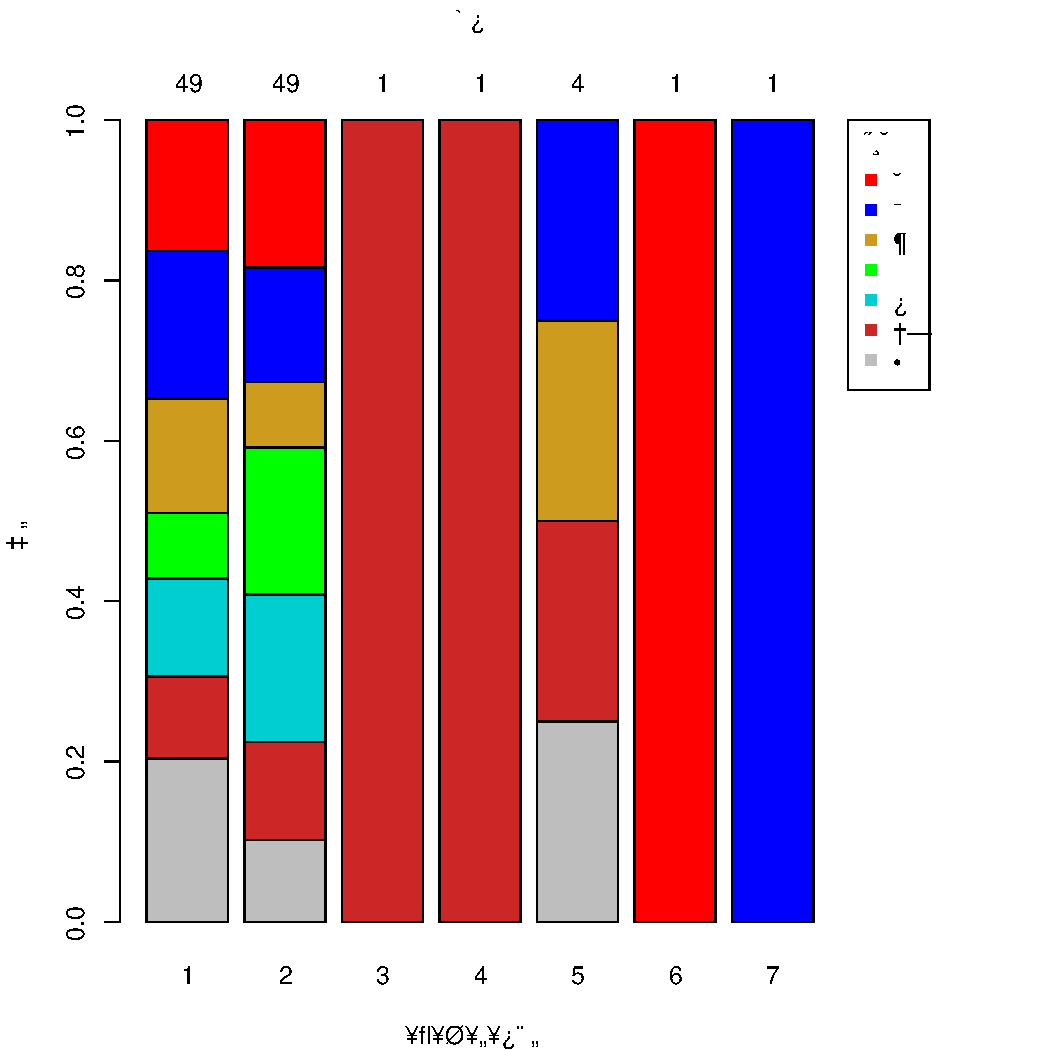
\includegraphics[height=4cm,width=6cm]{../figure/norm-eucl-cent-7-day.pdf}
}\\
\subfigure[クラスタ数 9 : 時間帯]{
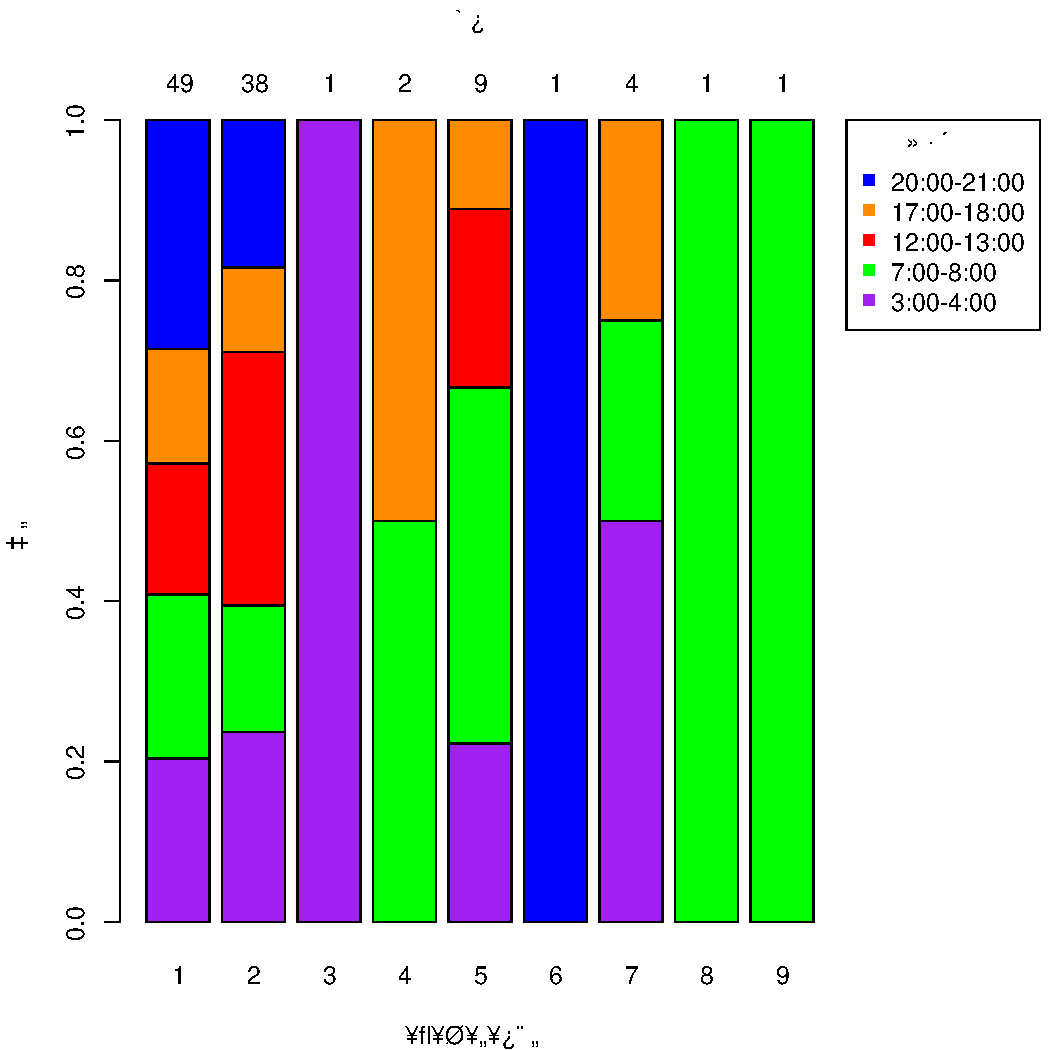
\includegraphics[height=4cm,width=6cm]{../figure/norm-eucl-cent-9-timezone.pdf}
}~
\subfigure[クラスタ数 9 : 曜日]{
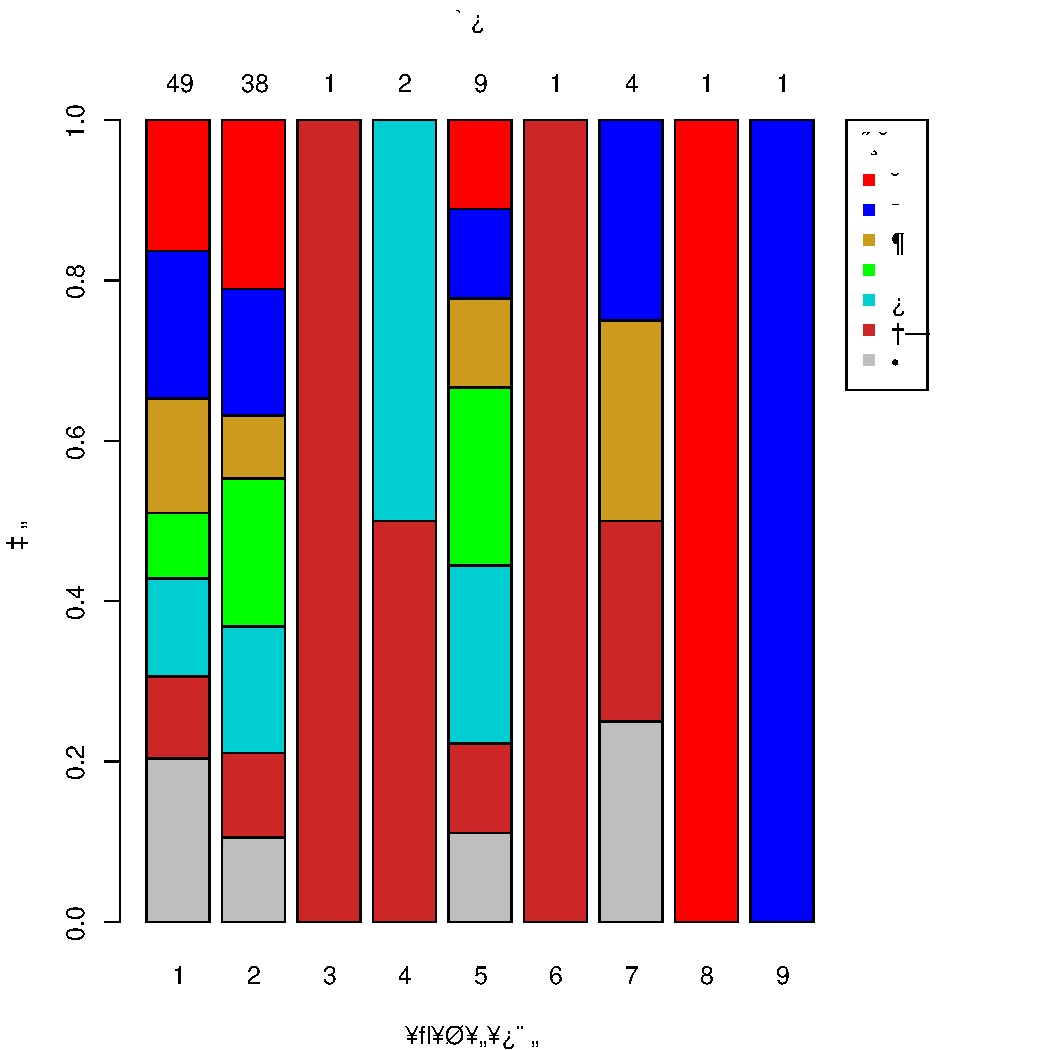
\includegraphics[height=4cm,width=6cm]{../figure/norm-eucl-cent-9-day.pdf}
}\\
\subfigure[クラスタ数 12 : 時間帯]{
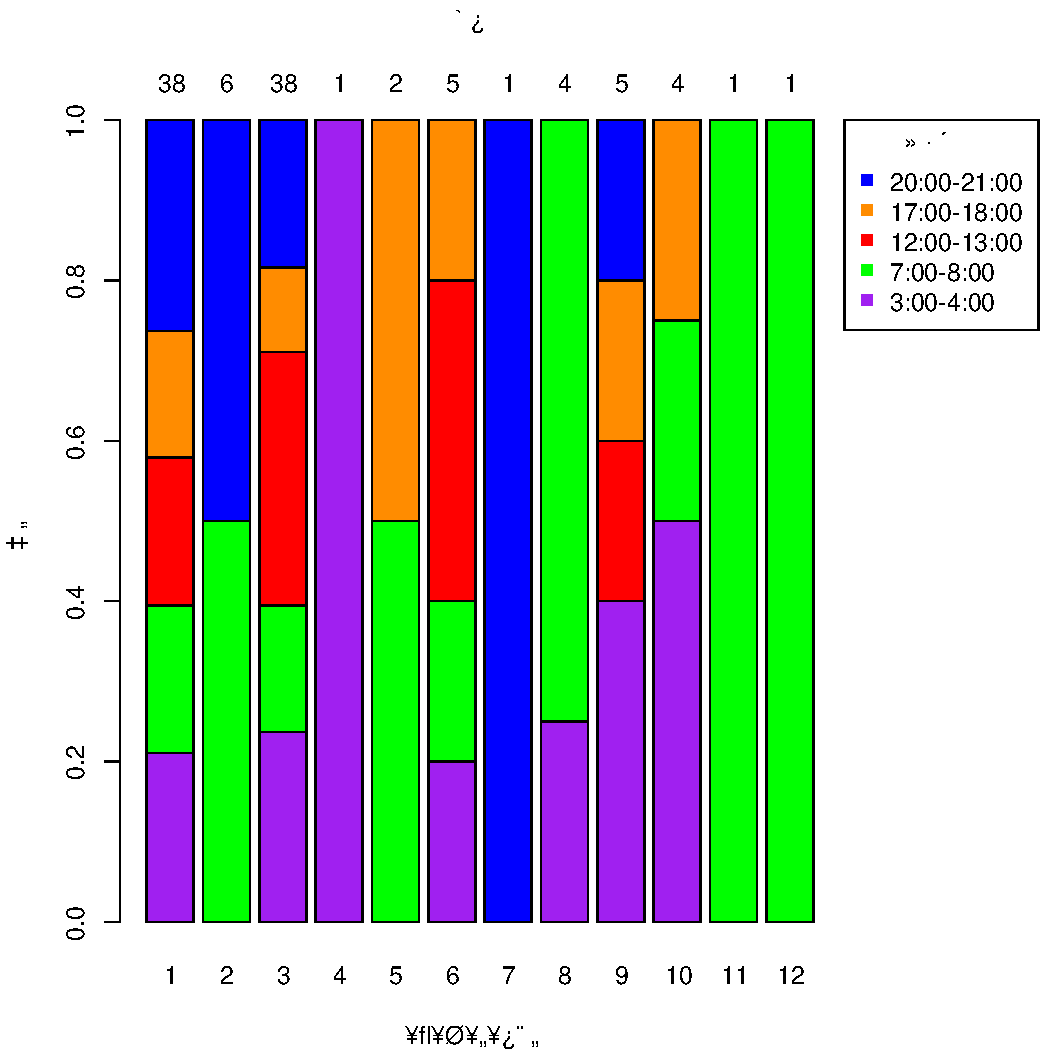
\includegraphics[height=4cm,width=6cm]{../figure/norm-eucl-cent-12-timezone.pdf}
}~
\subfigure[クラスタ数 12 : 曜日]{
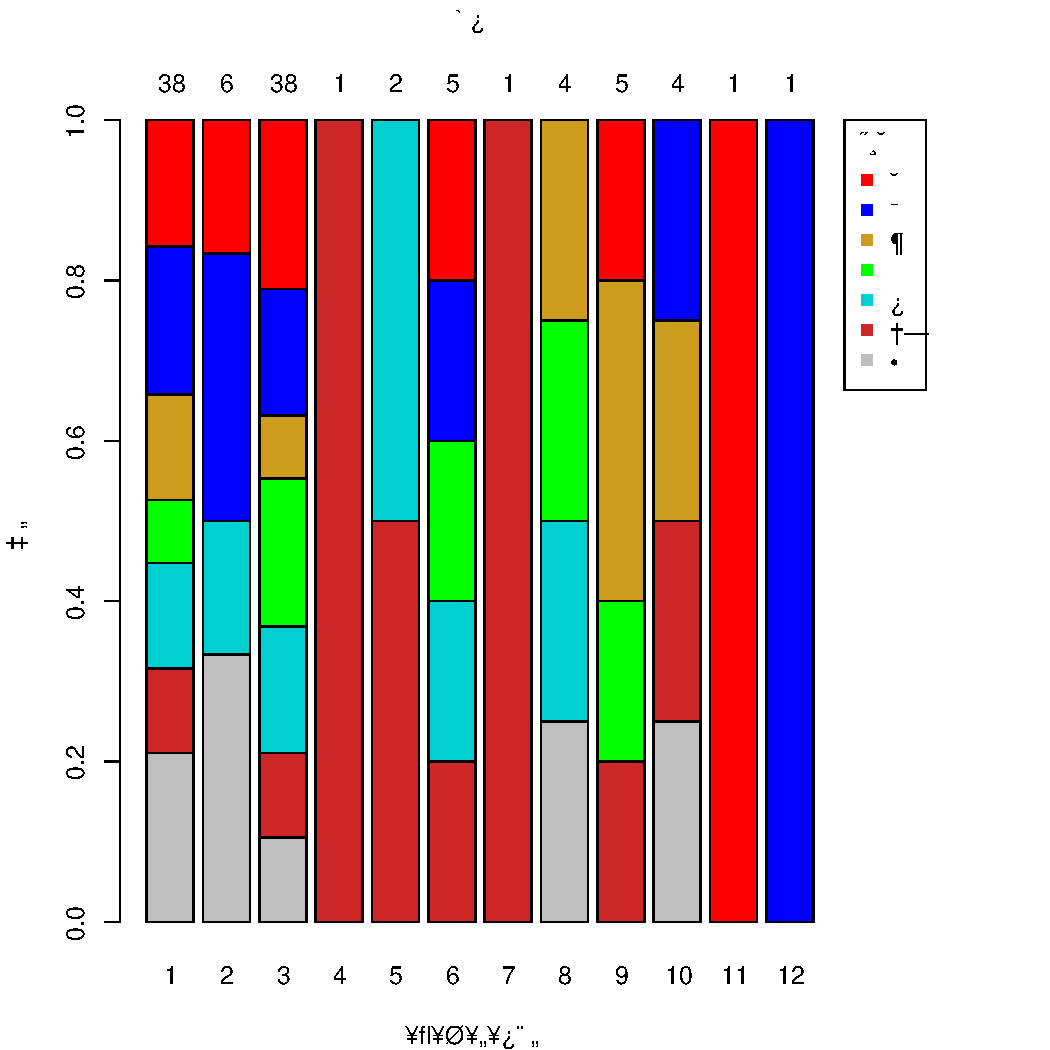
\includegraphics[height=4cm,width=6cm]{../figure/norm-eucl-cent-12-day.pdf}
}\\
\subfigure[クラスタ数 15 : 時間帯]{
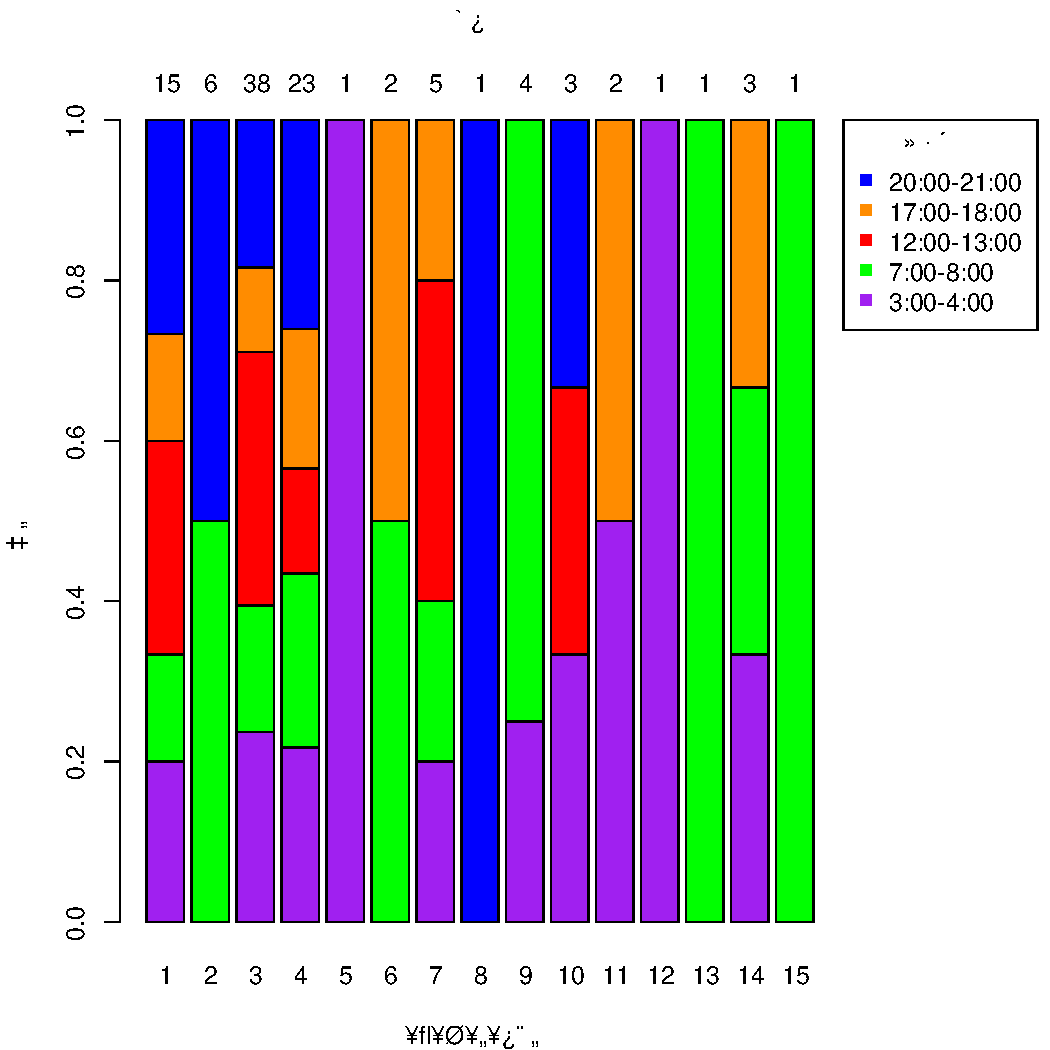
\includegraphics[height=4cm,width=6cm]{../figure/norm-eucl-cent-15-timezone.pdf}
}~
\subfigure[クラスタ数 15 : 曜日]{
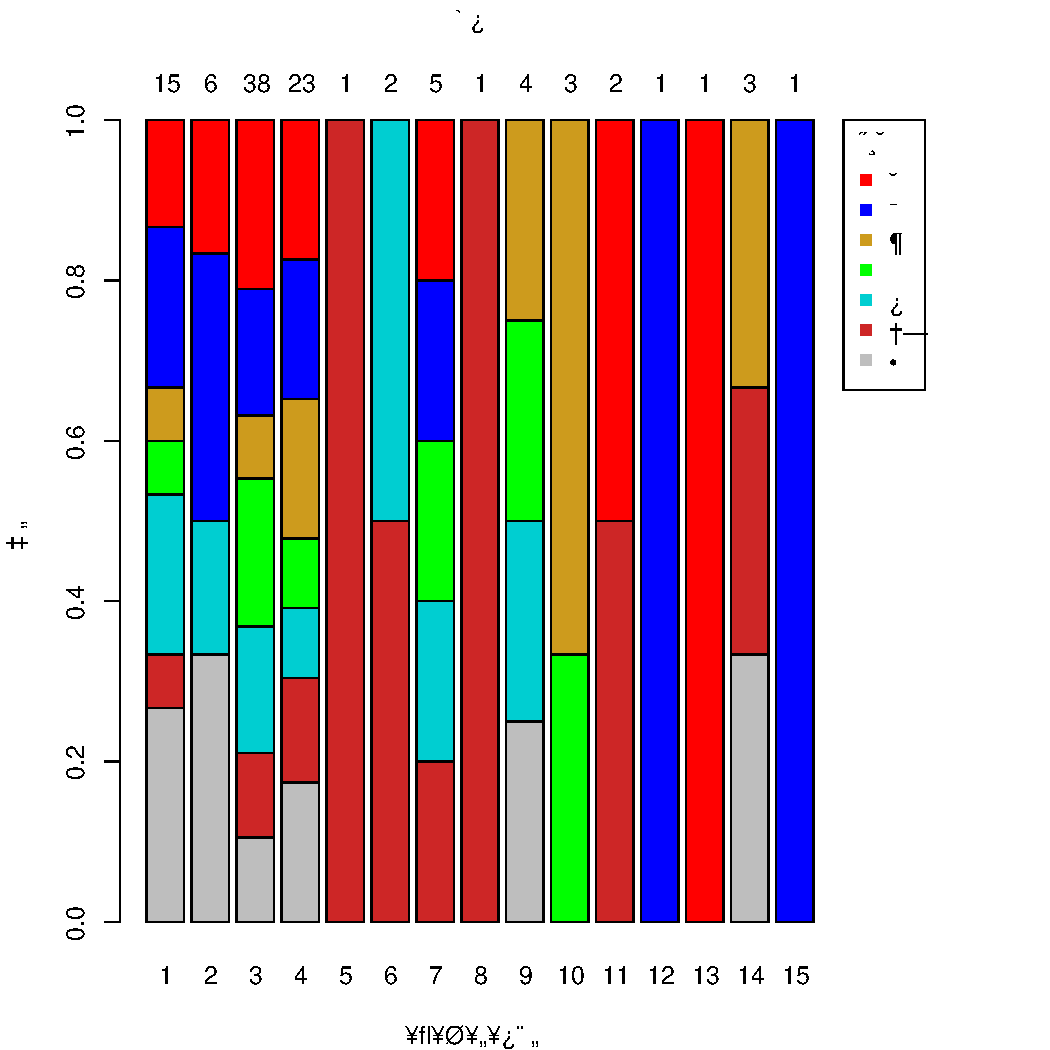
\includegraphics[height=4cm,width=6cm]{../figure/norm-eucl-cent-15-day.pdf}
}\\
\caption{実測値データに対する,ユークリッド距離と重心法によるクラスタリング}
\label{cluster1}
\end{center}
\end{figure}
\begin{figure}[tb]
\begin{center}
\subfigure[クラスタ数 6 : 時間帯]{
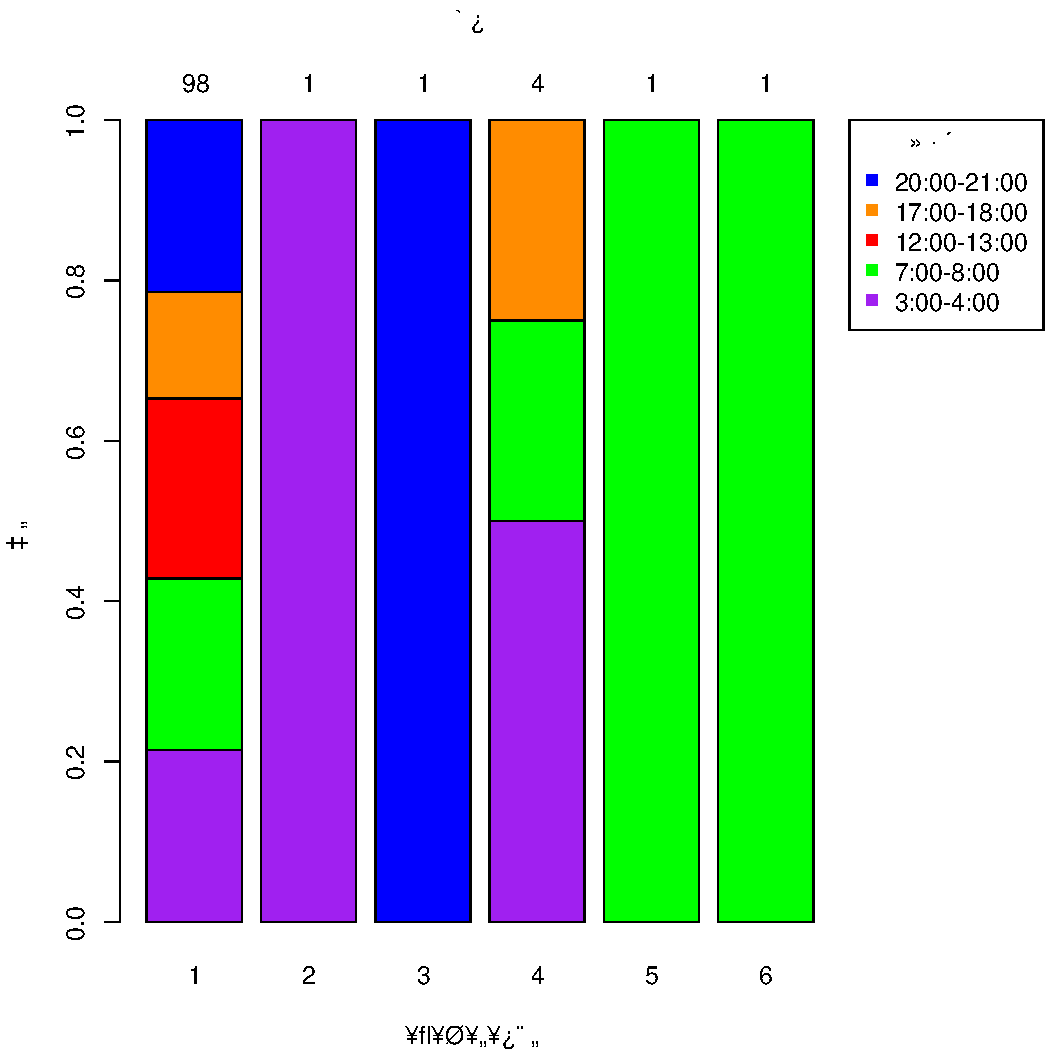
\includegraphics[height=4cm,width=6cm]{../figure/norm-eucl-sing-6-timezone.pdf}
}~
\subfigure[クラスタ数 6 : 曜日]{
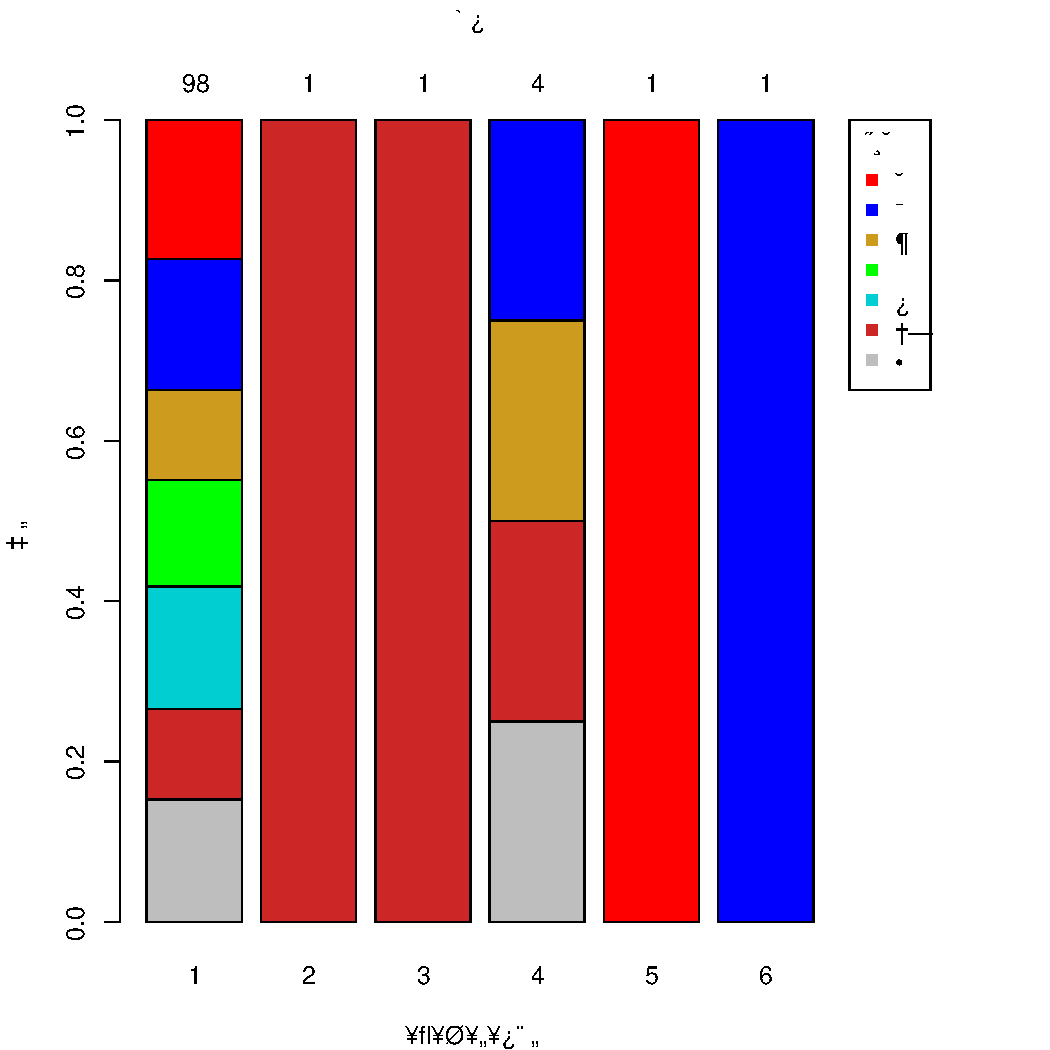
\includegraphics[height=4cm,width=6cm]{../figure/norm-eucl-sing-6-day.pdf}
}\\
\subfigure[クラスタ数 7 : 時間帯]{
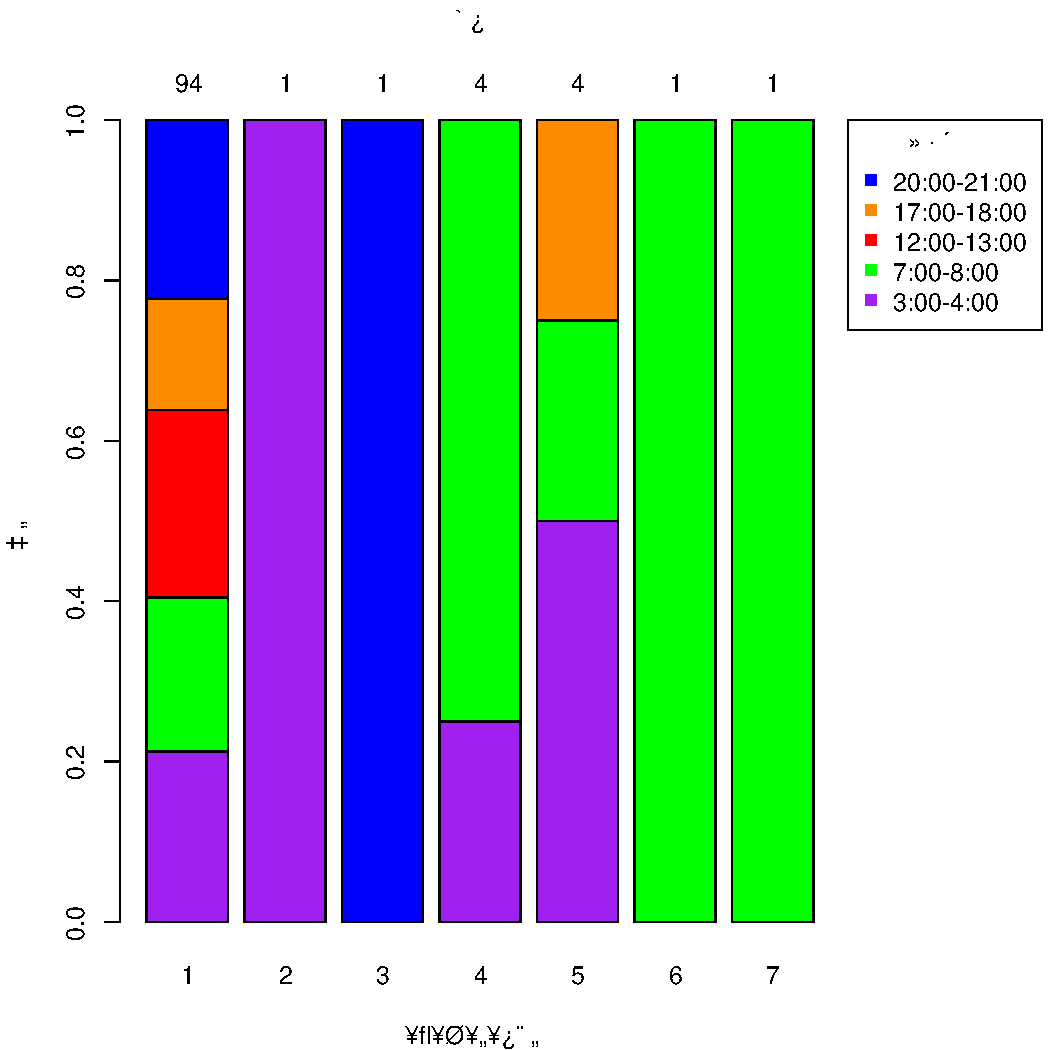
\includegraphics[height=4cm,width=6cm]{../figure/norm-eucl-sing-7-timezone.pdf}
}~
\subfigure[クラスタ数 7 : 曜日]{
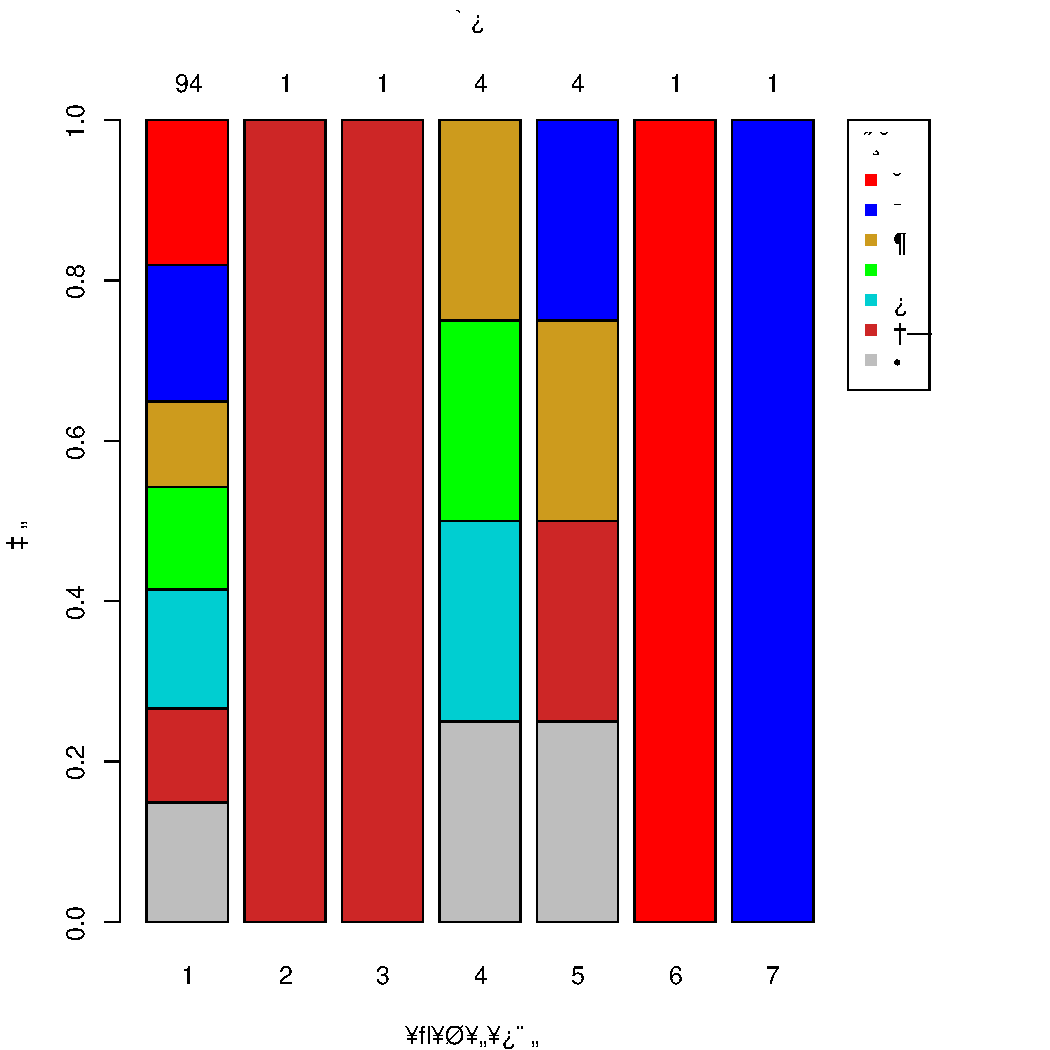
\includegraphics[height=4cm,width=6cm]{../figure/norm-eucl-sing-7-day.pdf}
}\\
\subfigure[クラスタ数 9 : 時間帯]{
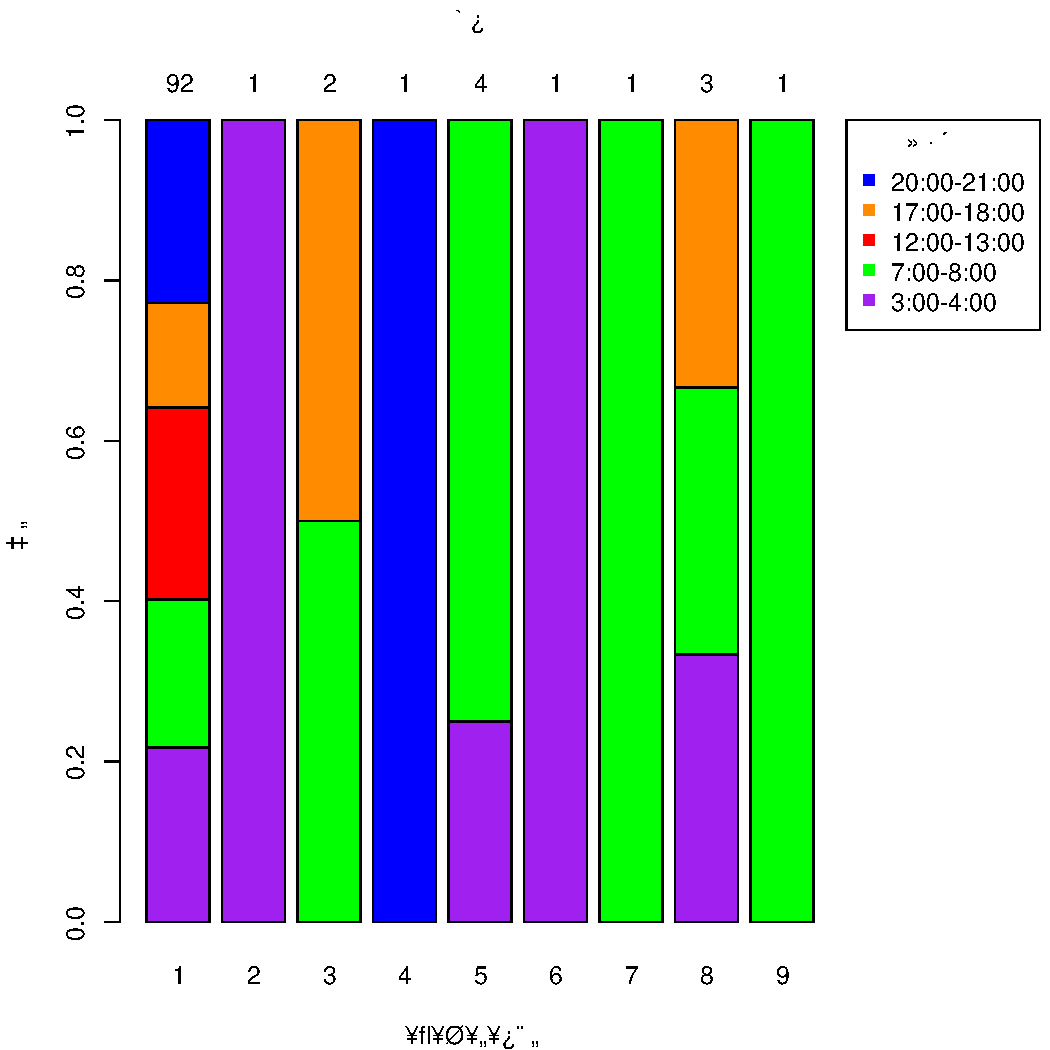
\includegraphics[height=4cm,width=6cm]{../figure/norm-eucl-sing-9-timezone.pdf}
}~
\subfigure[クラスタ数 9 : 曜日]{
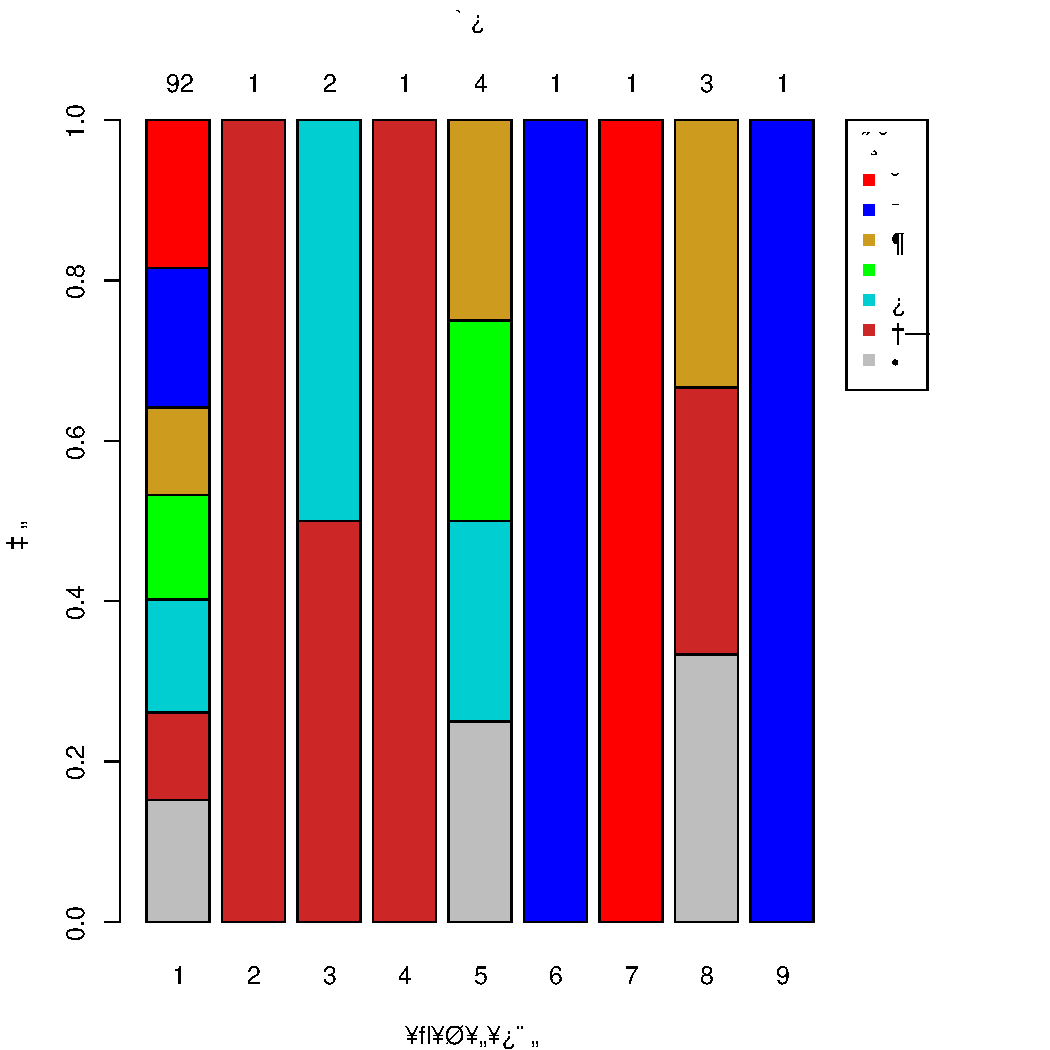
\includegraphics[height=4cm,width=6cm]{../figure/norm-eucl-sing-9-day.pdf}
}\\
\subfigure[クラスタ数 12 : 時間帯]{
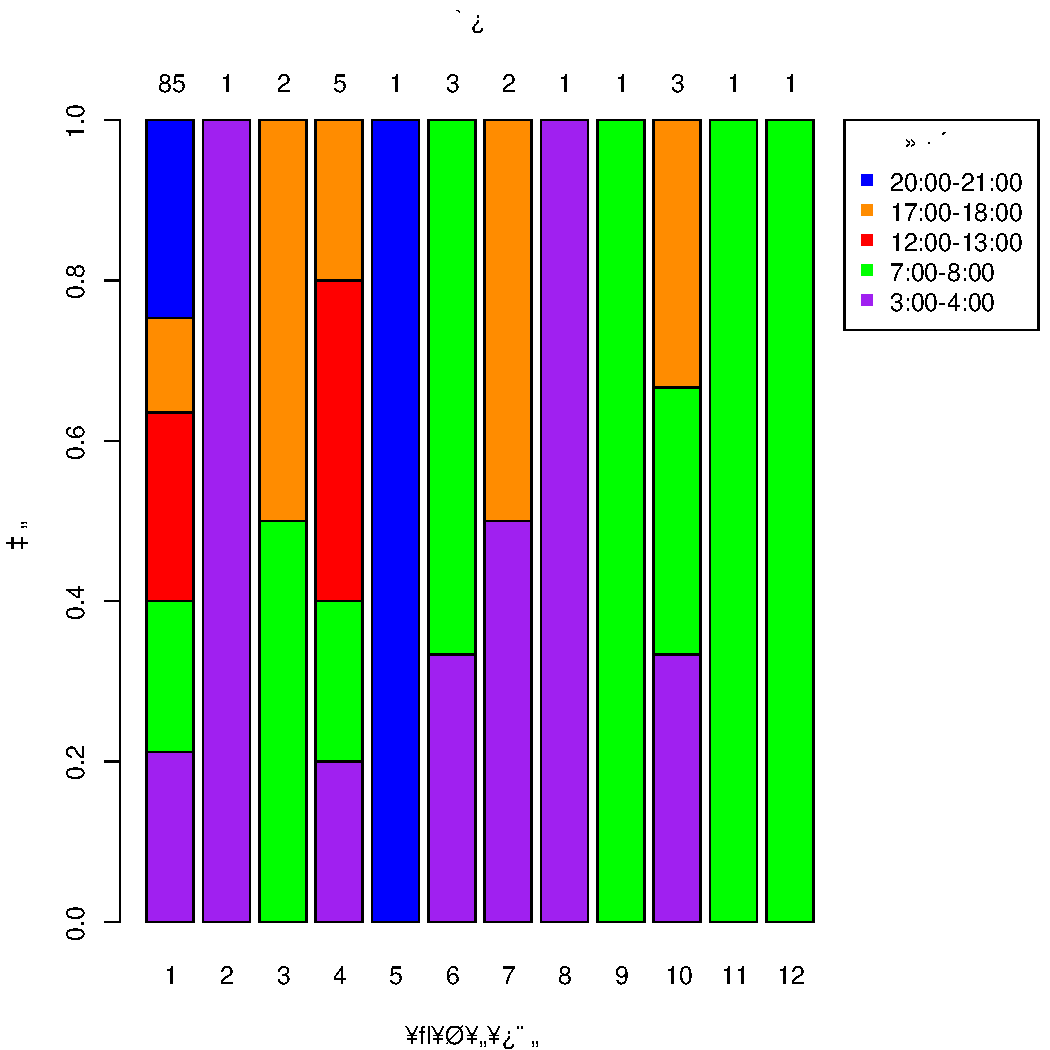
\includegraphics[height=4cm,width=6cm]{../figure/norm-eucl-sing-12-timezone.pdf}
}~
\subfigure[クラスタ数 12 : 曜日]{
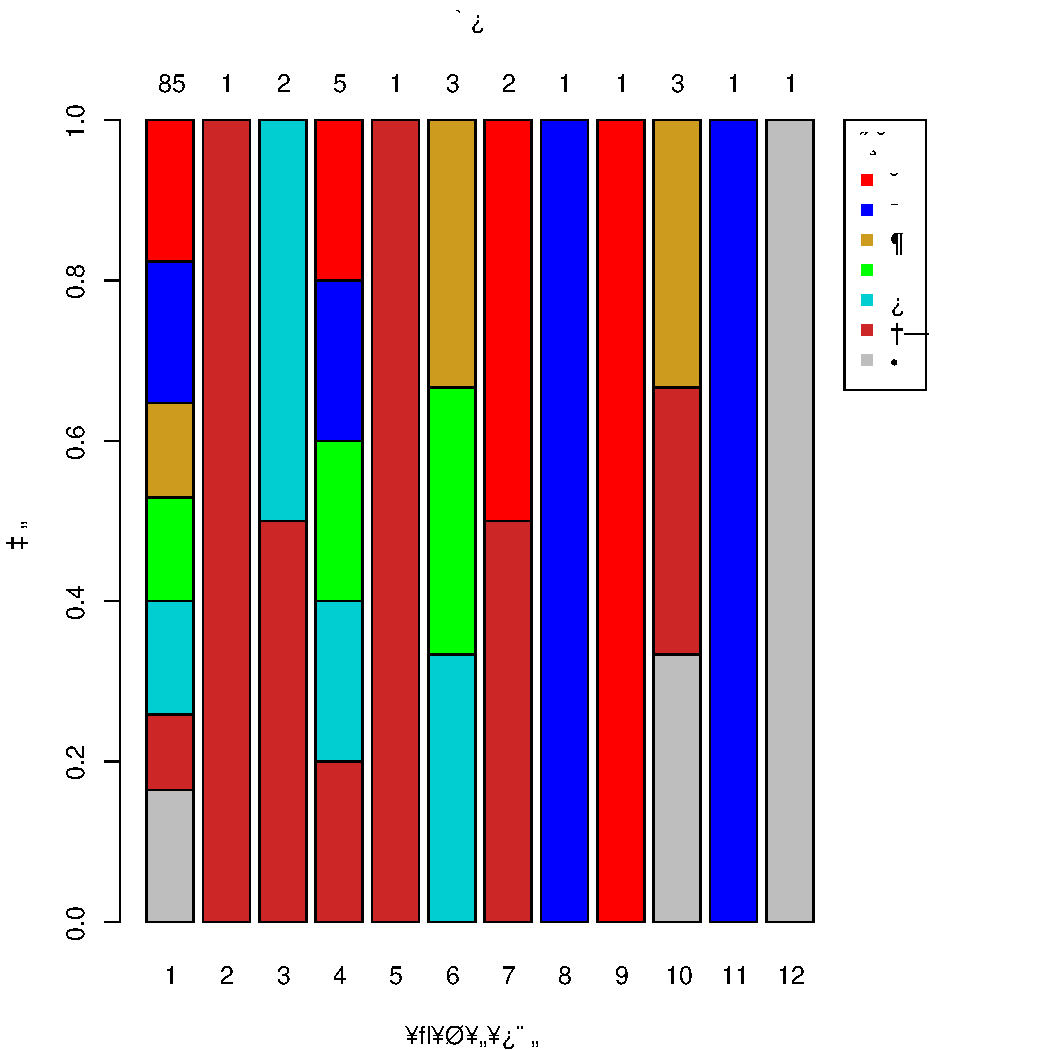
\includegraphics[height=4cm,width=6cm]{../figure/norm-eucl-sing-12-day.pdf}
}\\
\subfigure[クラスタ数 15 : 時間帯]{
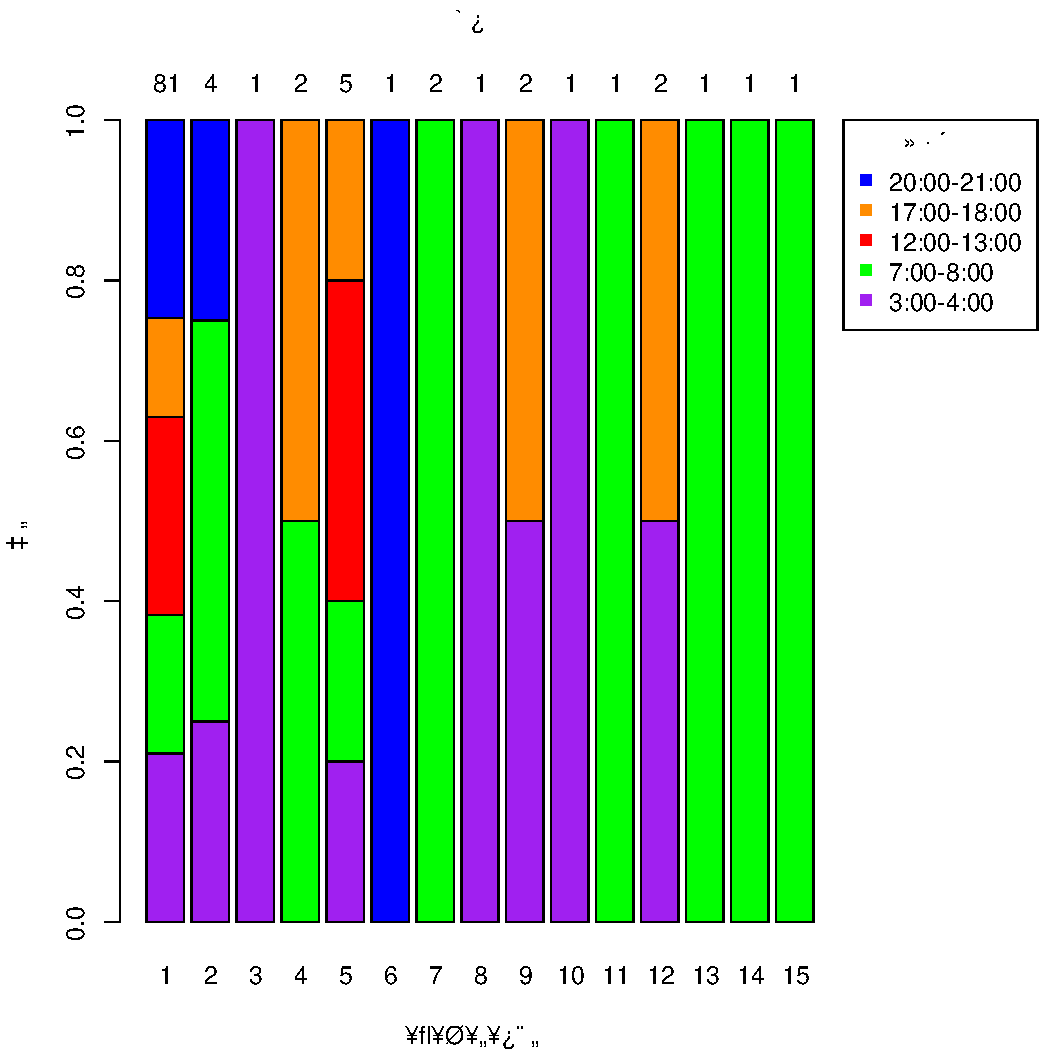
\includegraphics[height=4cm,width=6cm]{../figure/norm-eucl-sing-15-timezone.pdf}
}~
\subfigure[クラスタ数 15 : 曜日]{
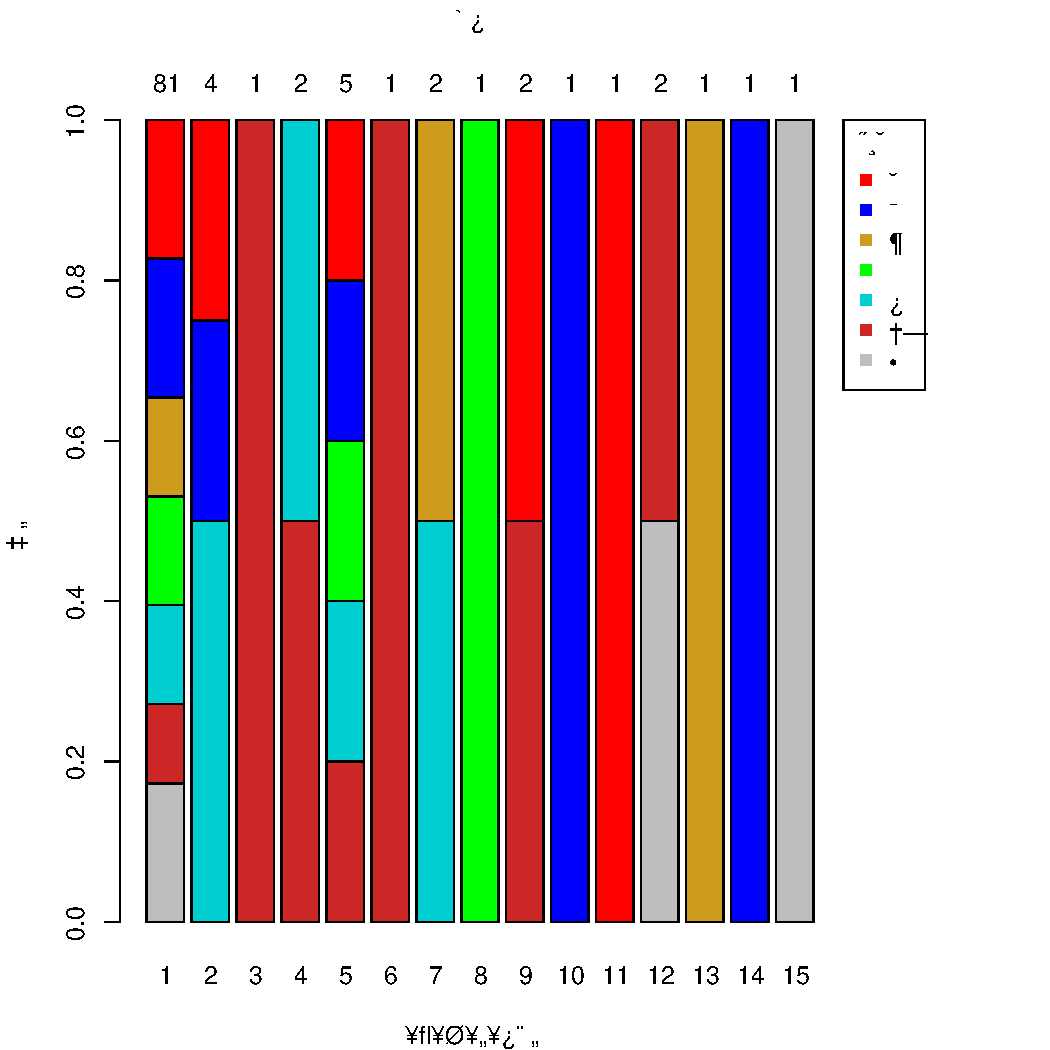
\includegraphics[height=4cm,width=6cm]{../figure/norm-eucl-sing-15-day.pdf}
}\\
\caption{実測値データに対する,ユークリッド距離と最近傍法によるクラスタリング}
\end{center}
\end{figure}
\begin{figure}[tb]
\begin{center}
\subfigure[クラスタ数 6 : 時間帯]{
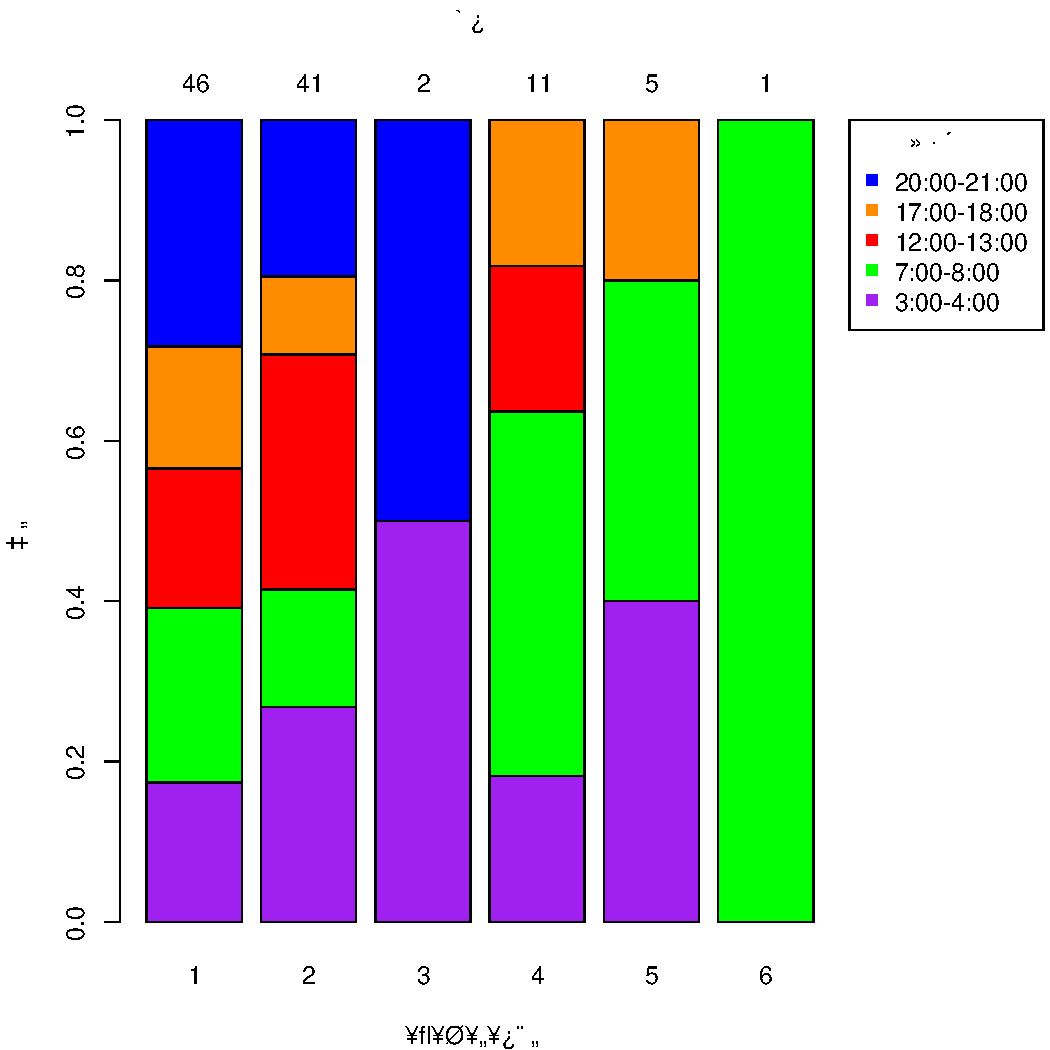
\includegraphics[height=4cm,width=6cm]{../figure/norm-eucl-ward-6-timezone.pdf}
}~
\subfigure[クラスタ数 6 : 曜日]{
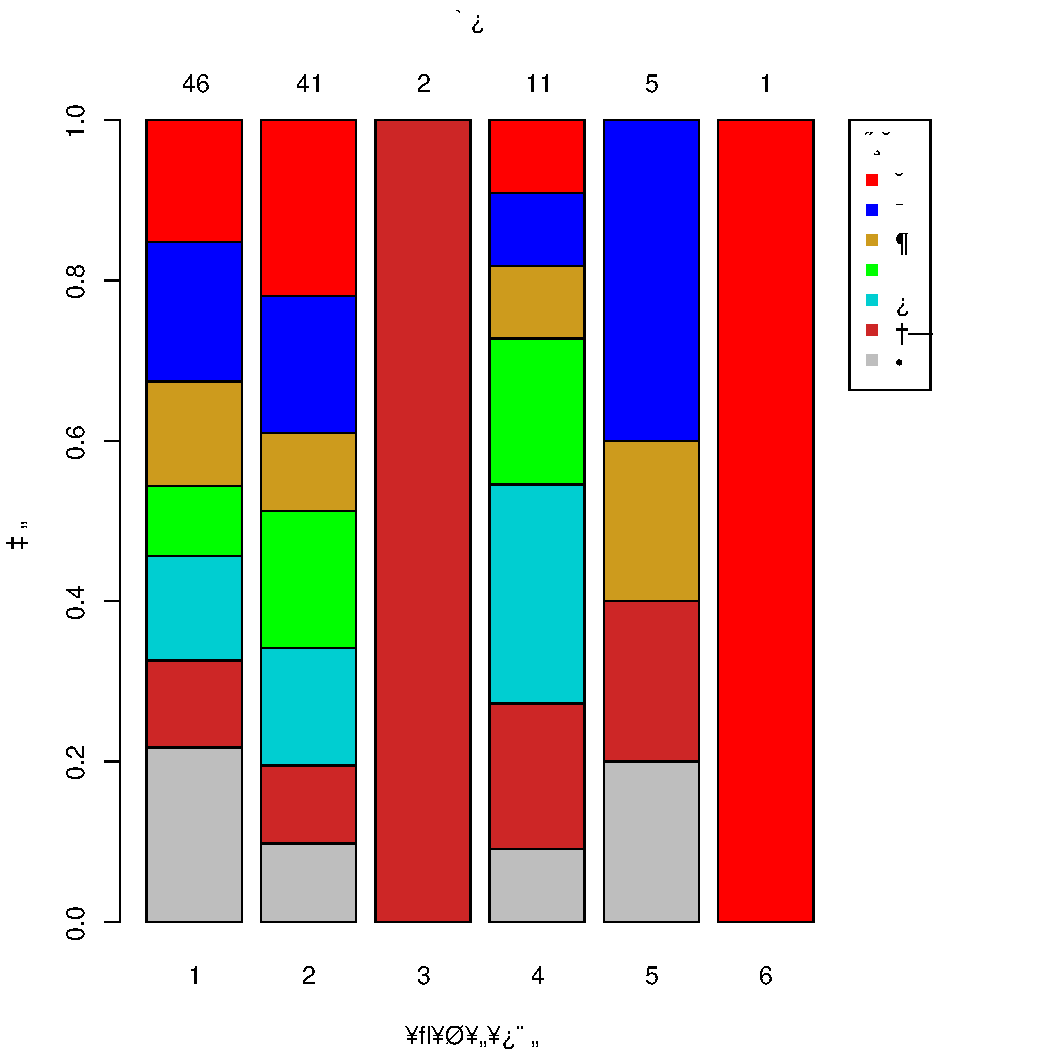
\includegraphics[height=4cm,width=6cm]{../figure/norm-eucl-ward-6-day.pdf}
}\\
\subfigure[クラスタ数 7 : 時間帯]{
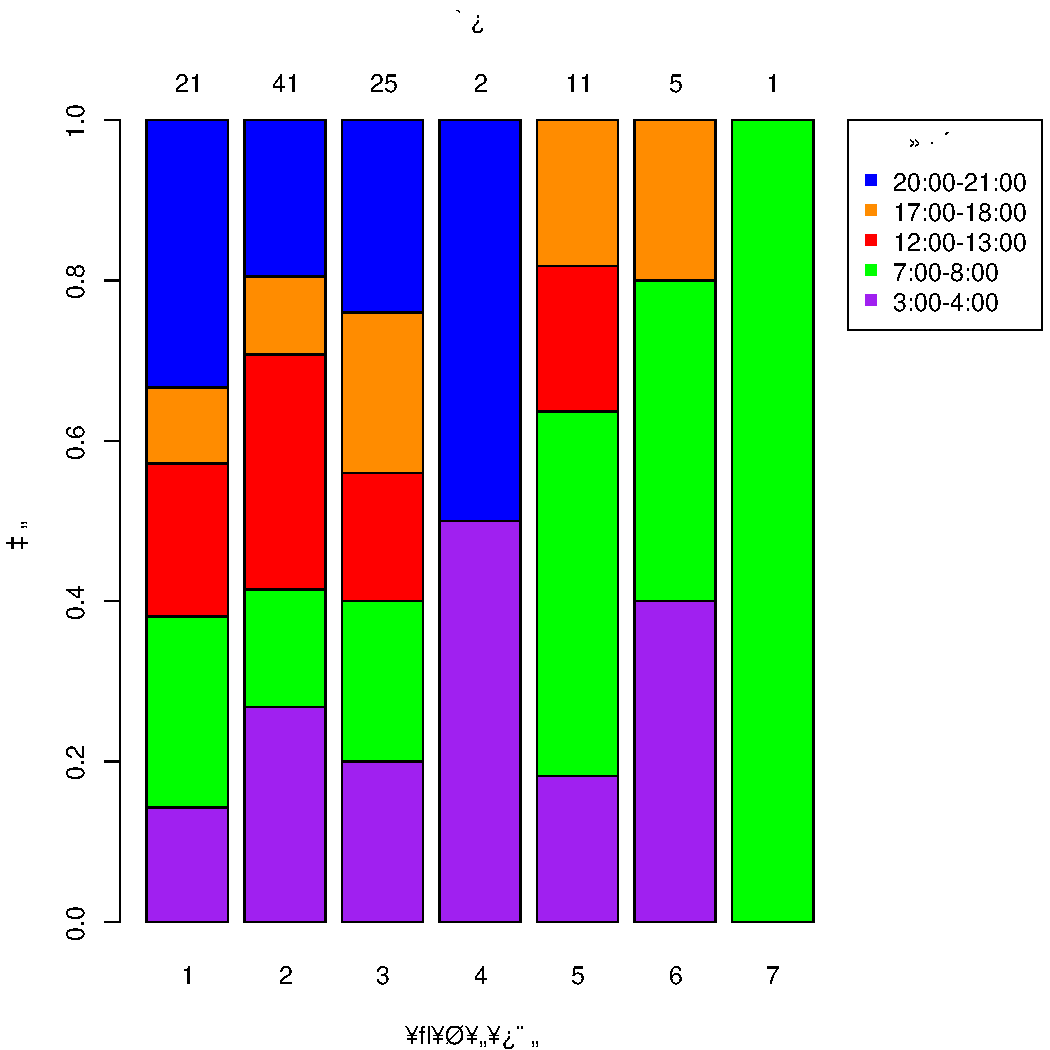
\includegraphics[height=4cm,width=6cm]{../figure/norm-eucl-ward-7-timezone.pdf}
}~
\subfigure[クラスタ数 7 : 曜日]{
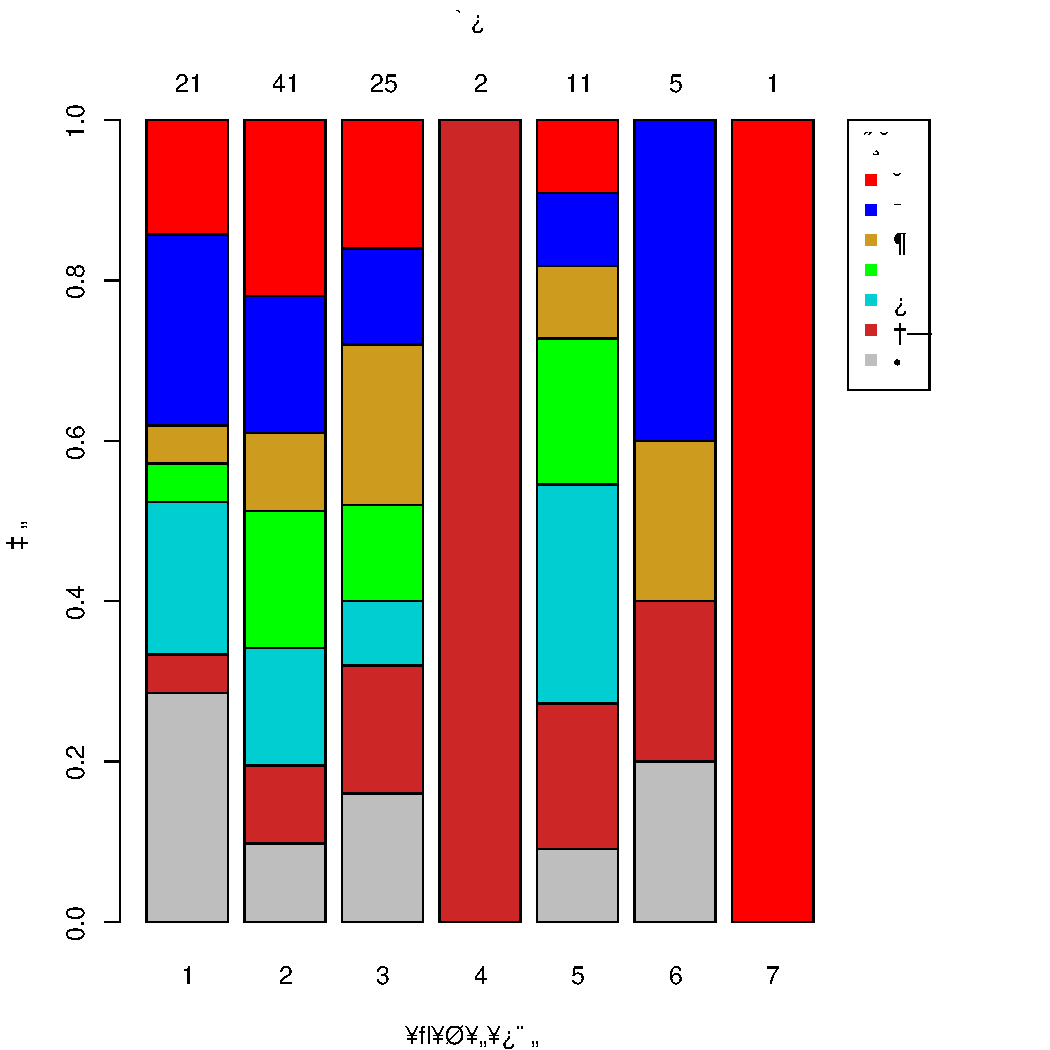
\includegraphics[height=4cm,width=6cm]{../figure/norm-eucl-ward-7-day.pdf}
}\\
\subfigure[クラスタ数 9 : 時間帯]{
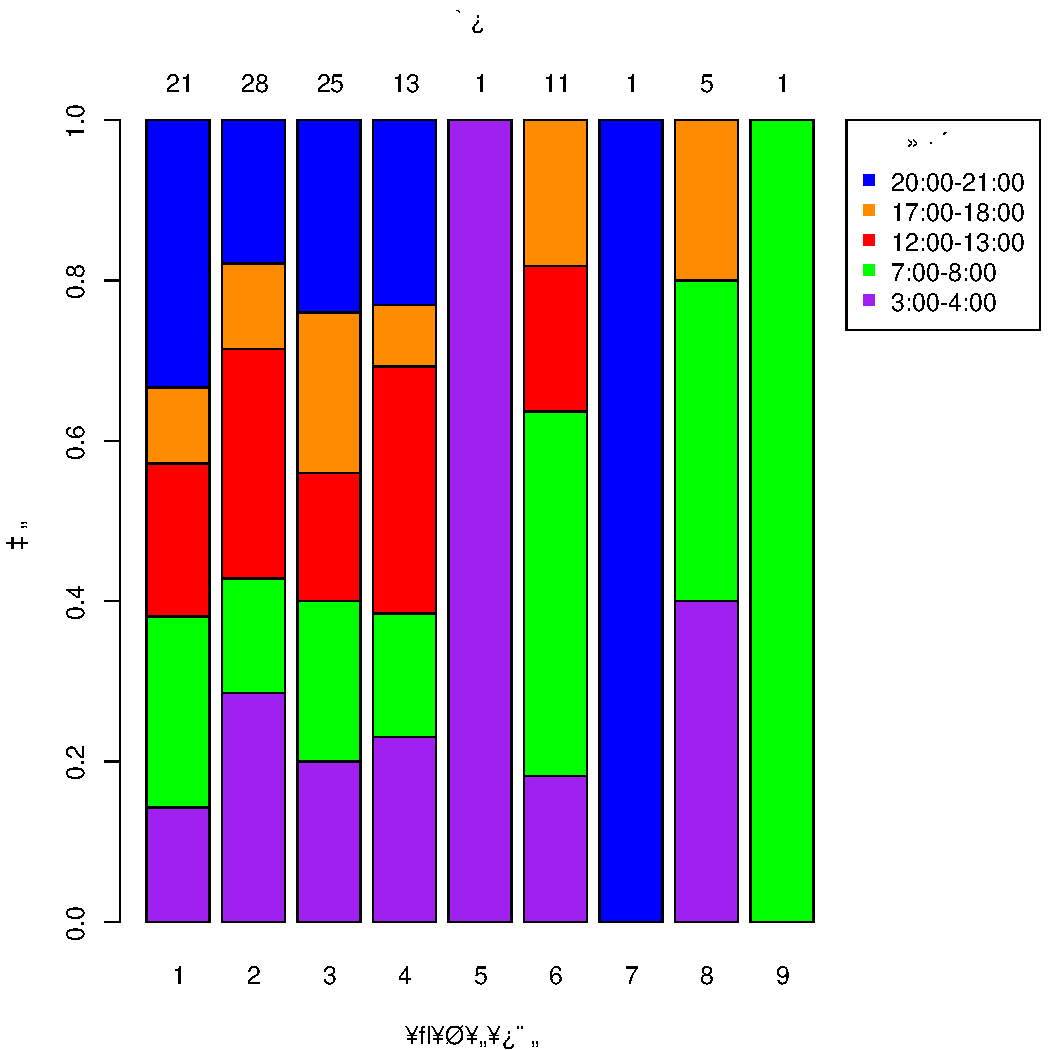
\includegraphics[height=4cm,width=6cm]{../figure/norm-eucl-ward-9-timezone.pdf}
}~
\subfigure[クラスタ数 9 : 曜日]{
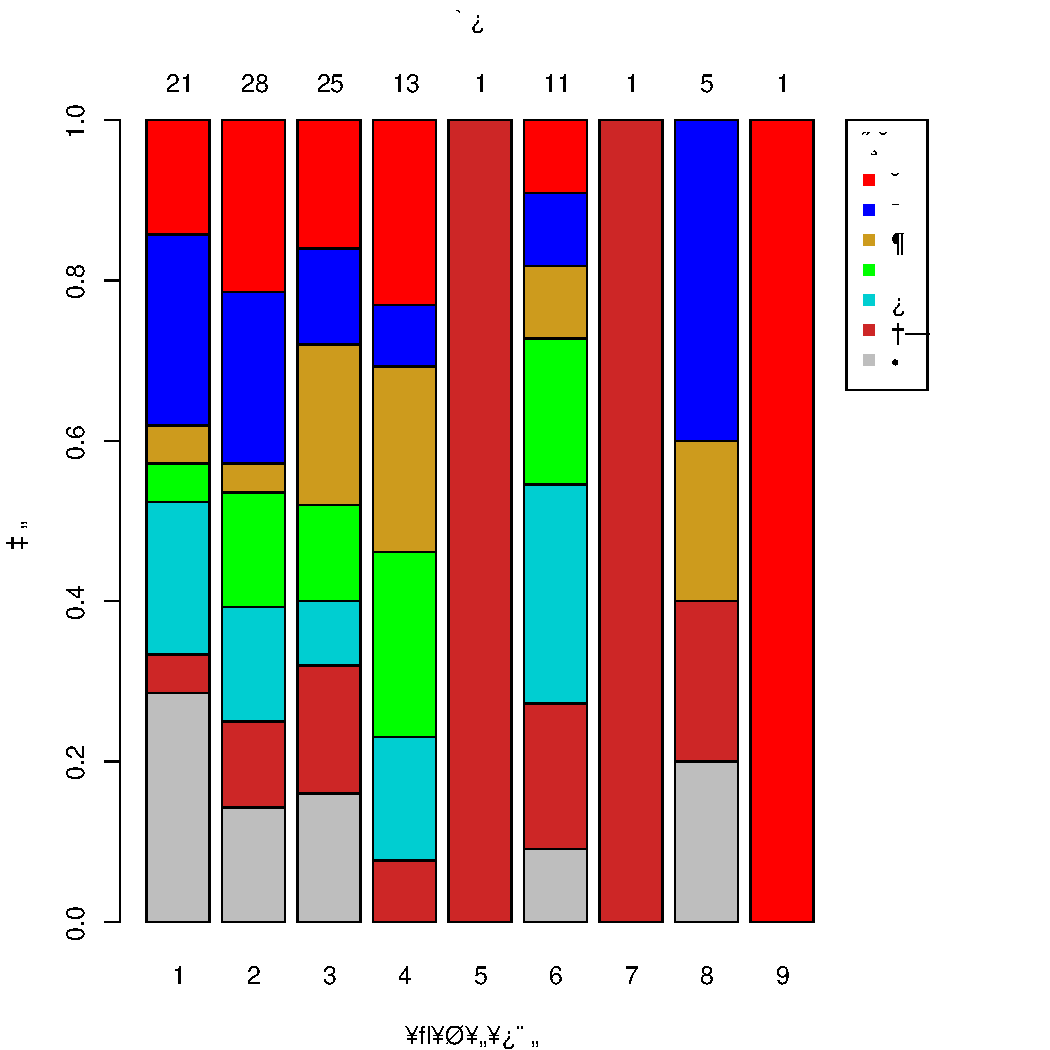
\includegraphics[height=4cm,width=6cm]{../figure/norm-eucl-ward-9-day.pdf}
}\\
\subfigure[クラスタ数 12 : 時間帯]{
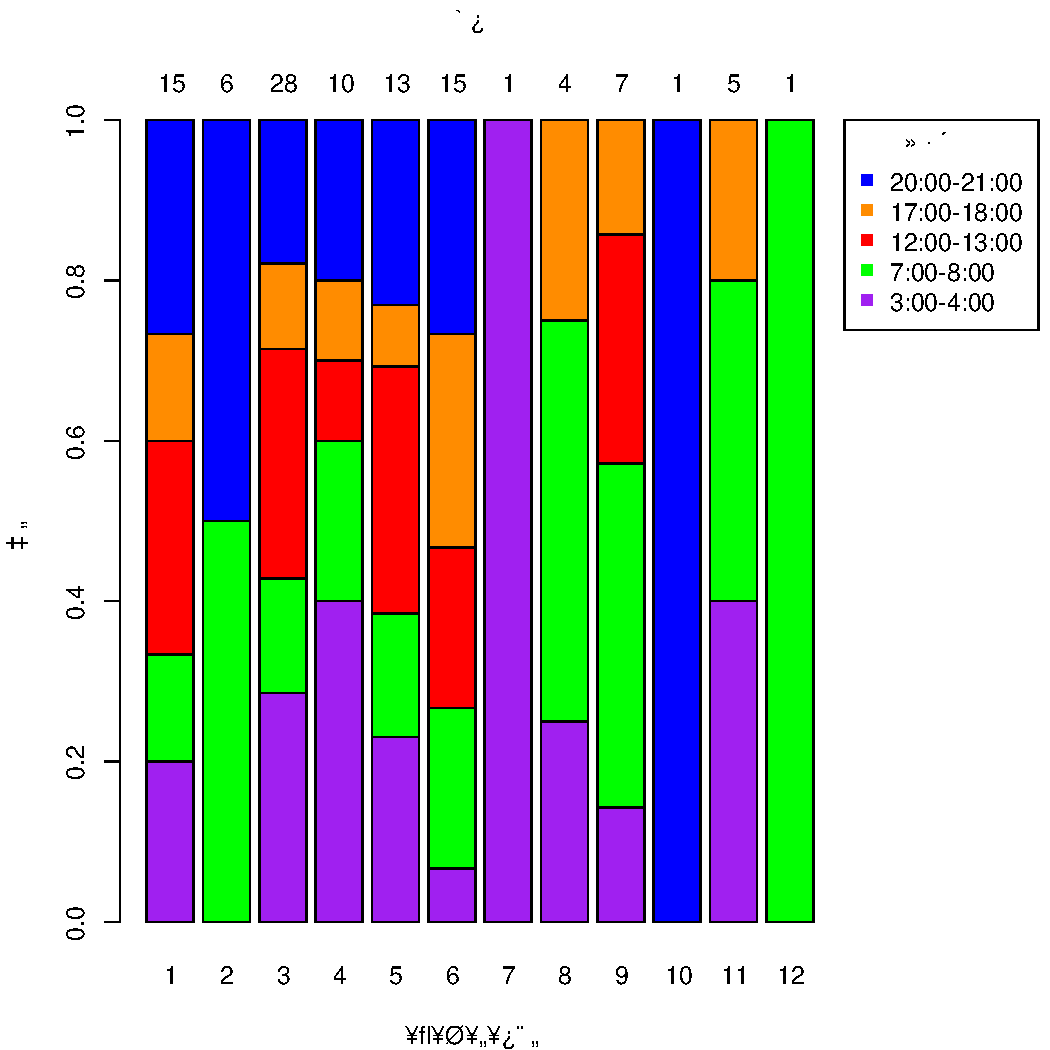
\includegraphics[height=4cm,width=6cm]{../figure/norm-eucl-ward-12-timezone.pdf}
}~
\subfigure[クラスタ数 12 : 曜日]{
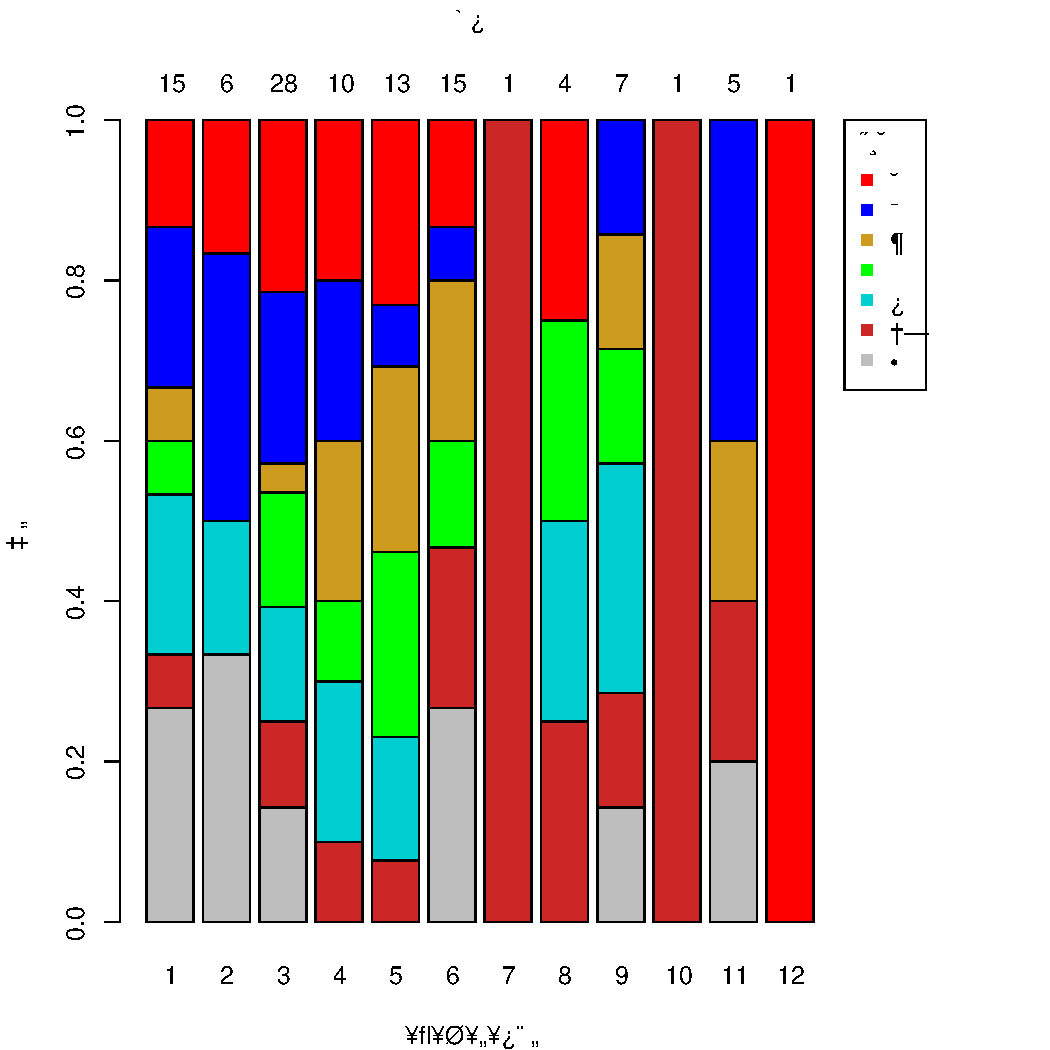
\includegraphics[height=4cm,width=6cm]{../figure/norm-eucl-ward-12-day.pdf}
}\\
\subfigure[クラスタ数 15 : 時間帯]{
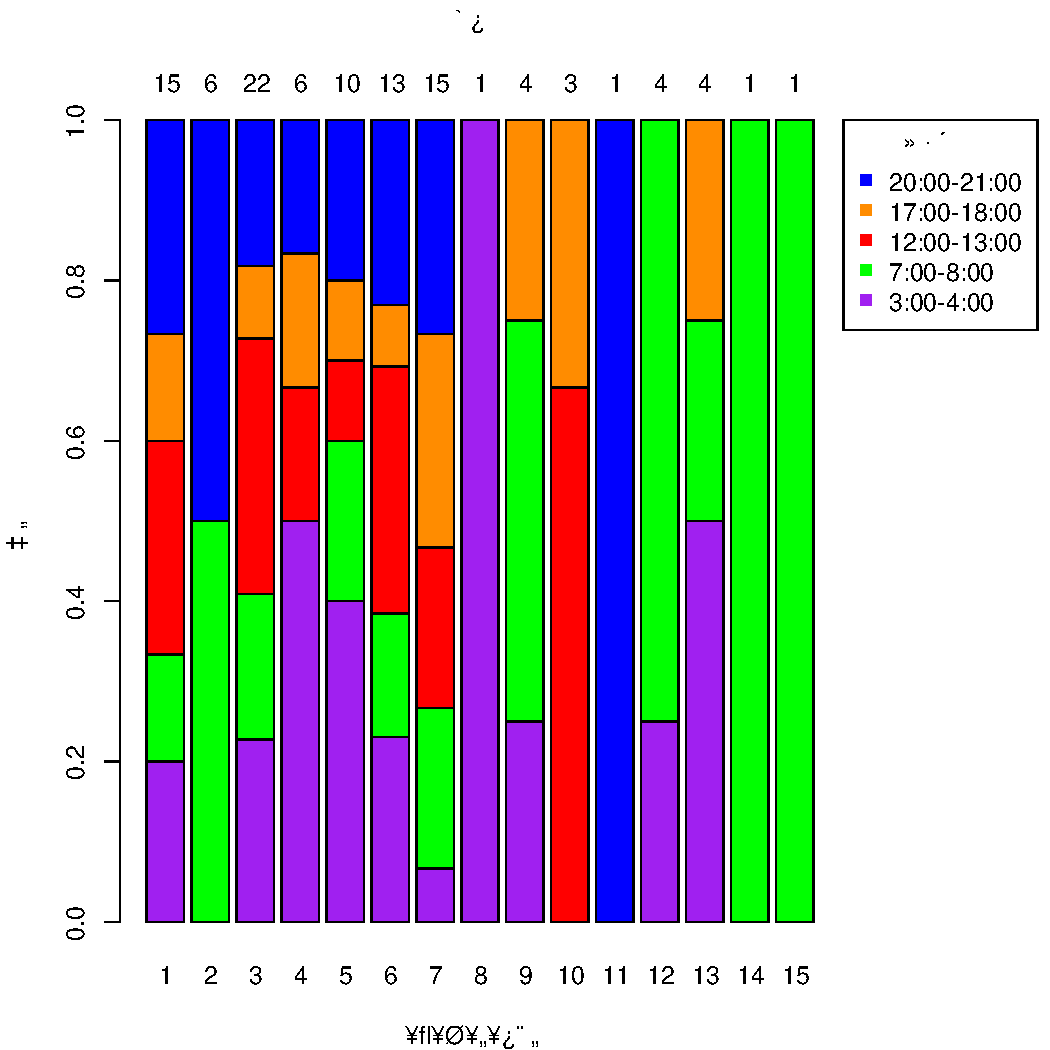
\includegraphics[height=4cm,width=6cm]{../figure/norm-eucl-ward-15-timezone.pdf}
}~
\subfigure[クラスタ数 15 : 曜日]{
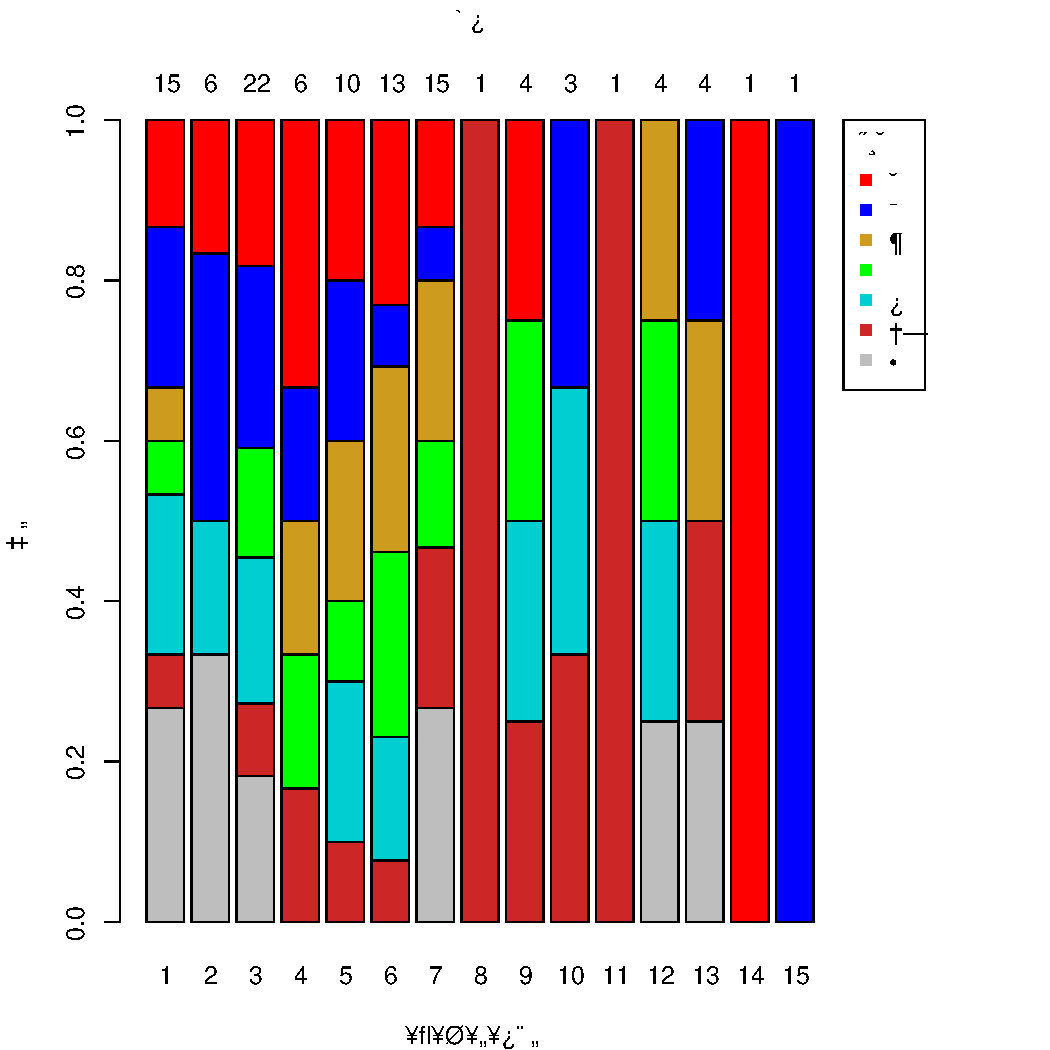
\includegraphics[height=4cm,width=6cm]{../figure/norm-eucl-ward-15-day.pdf}
}\\
\caption{実測値データに対する,ユークリッド距離とウォード法によるクラスタリング}
\end{center}
\end{figure}
\begin{figure}[tb]
\begin{center}
\subfigure[クラスタ数 6 : 時間帯]{
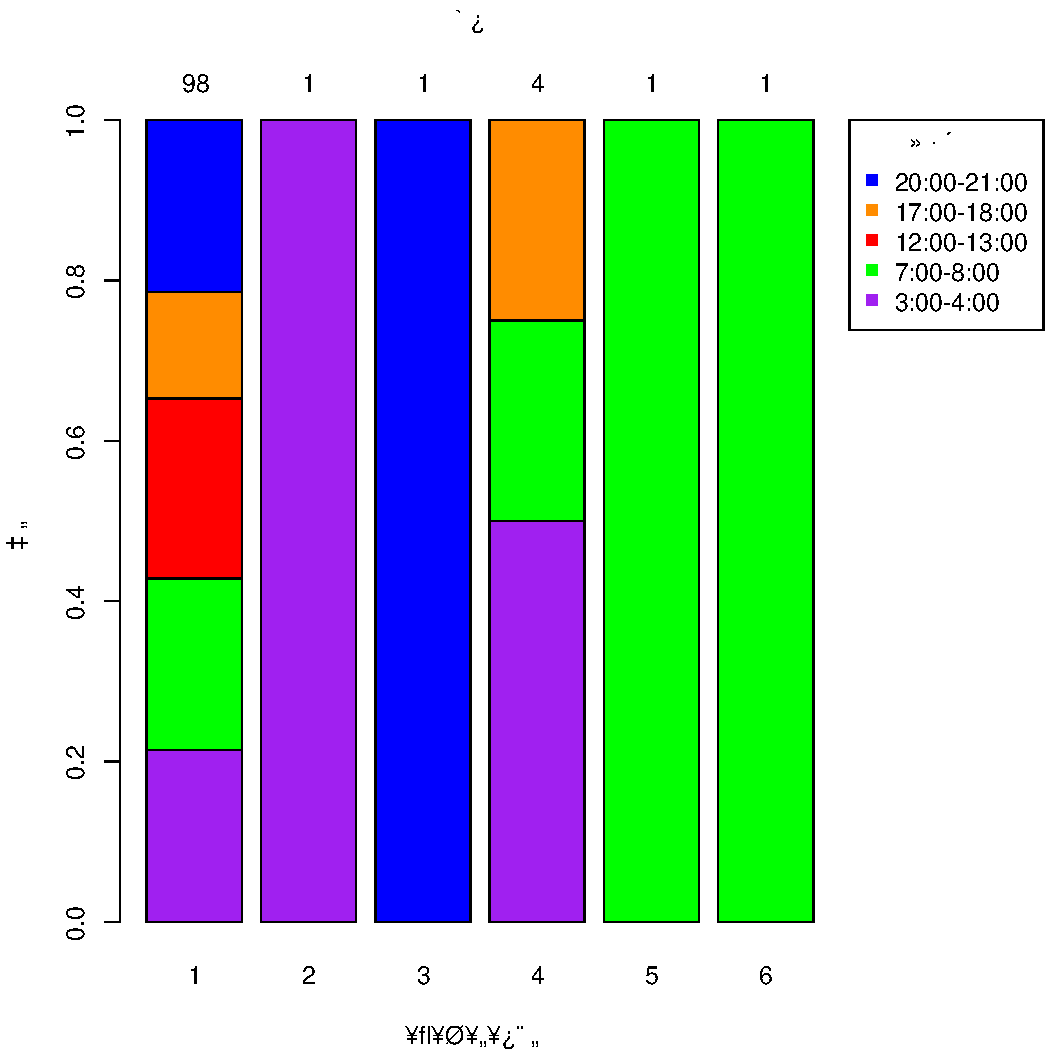
\includegraphics[height=4cm,width=6cm]{../figure/norm-manh-cent-6-timezone.pdf}
}~
\subfigure[クラスタ数 6 : 曜日]{
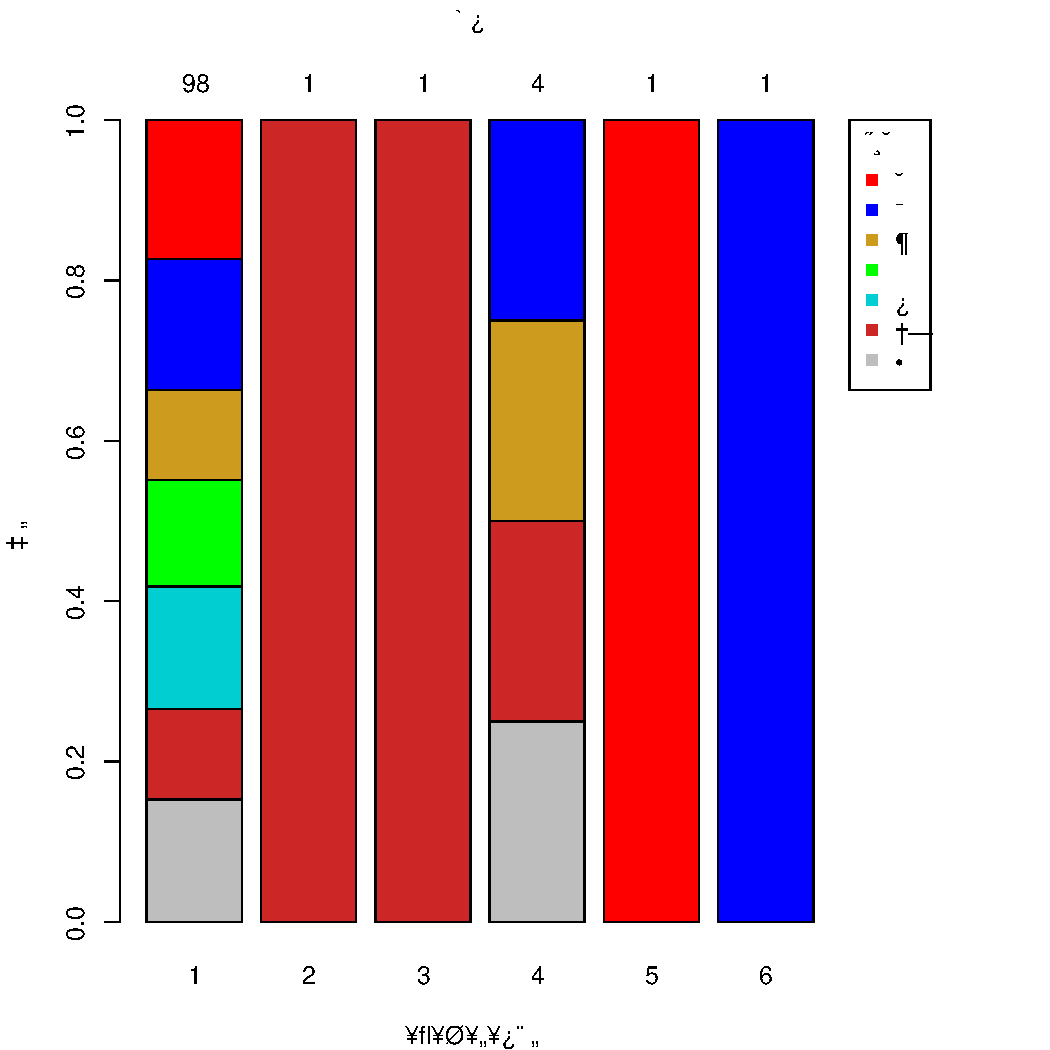
\includegraphics[height=4cm,width=6cm]{../figure/norm-manh-cent-6-day.pdf}
}\\
\subfigure[クラスタ数 7 : 時間帯]{
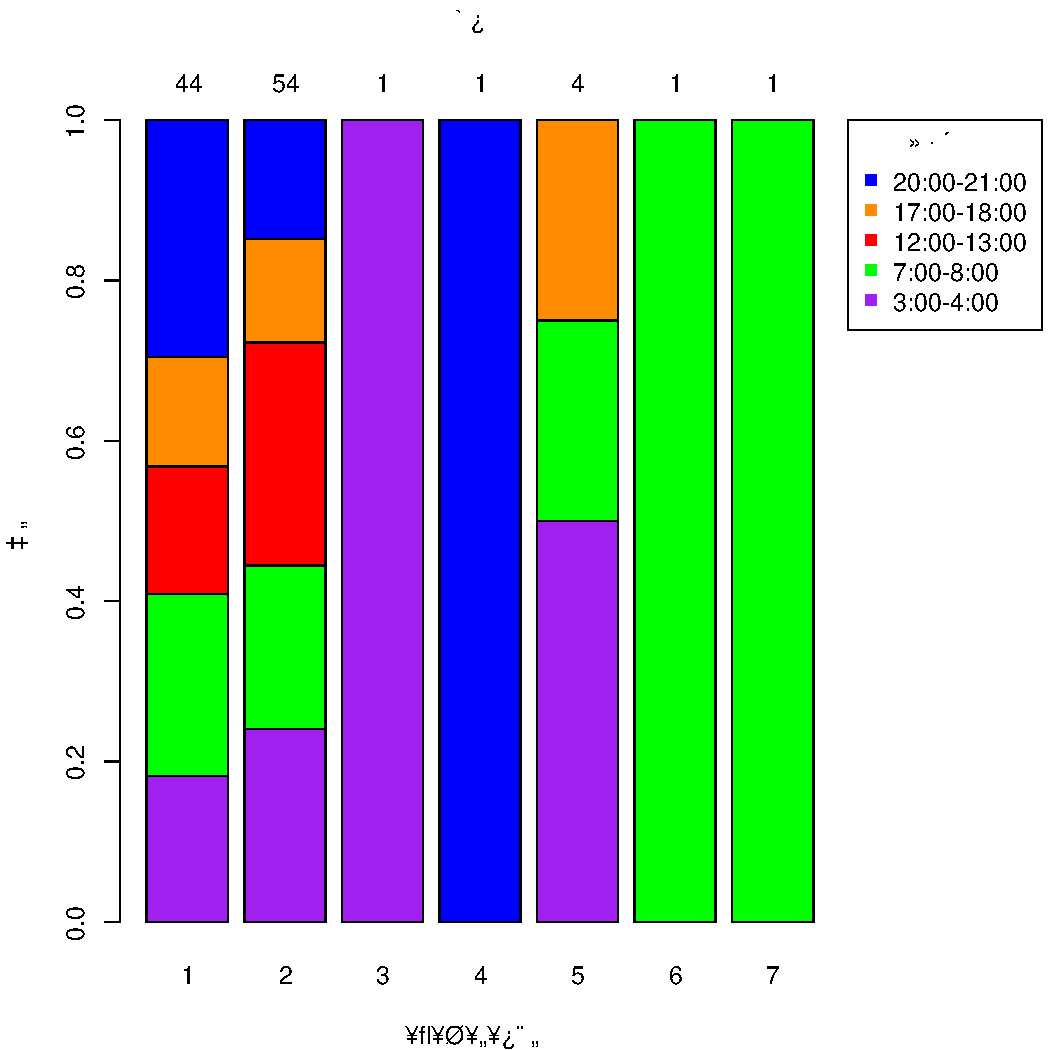
\includegraphics[height=4cm,width=6cm]{../figure/norm-manh-cent-7-timezone.pdf}
}~
\subfigure[クラスタ数 7 : 曜日]{
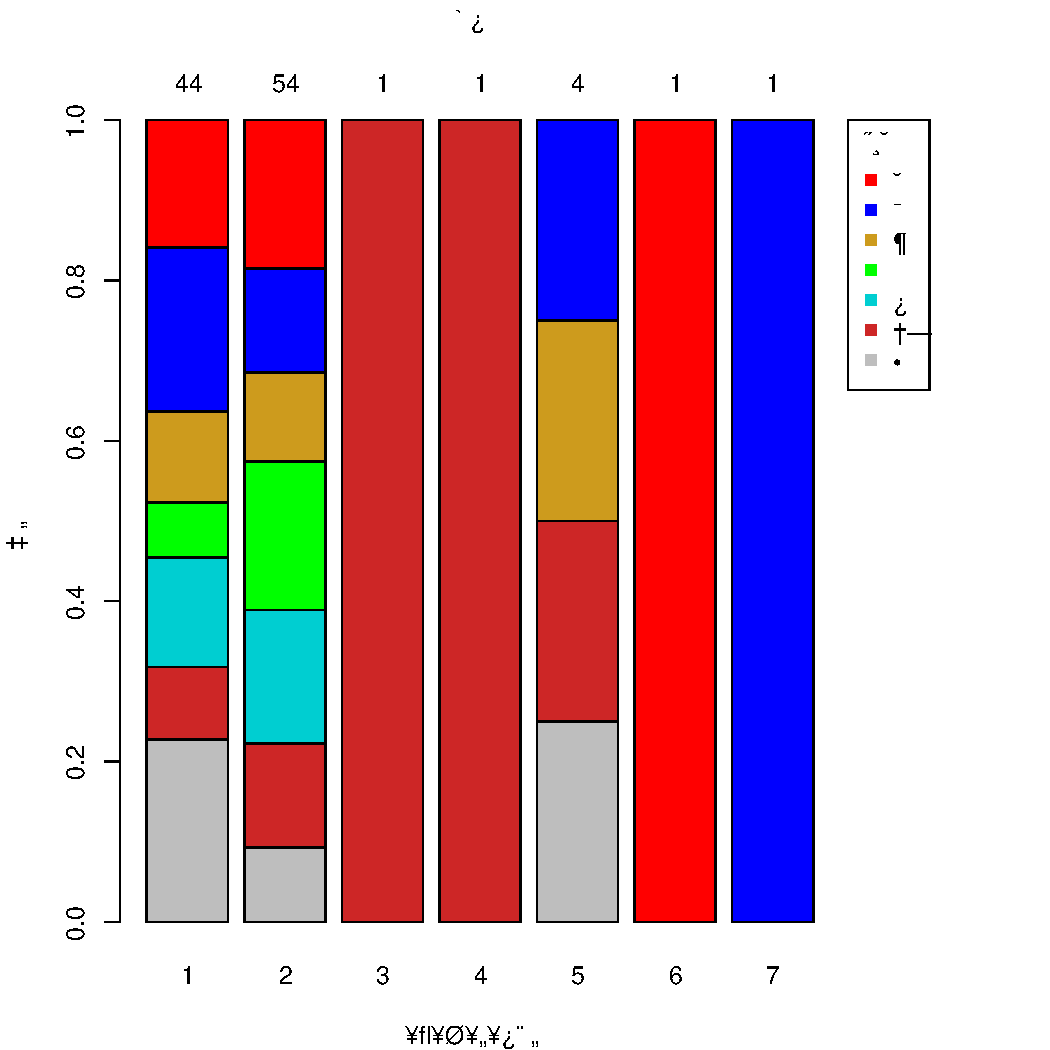
\includegraphics[height=4cm,width=6cm]{../figure/norm-manh-cent-7-day.pdf}
}\\
\subfigure[クラスタ数 9 : 時間帯]{
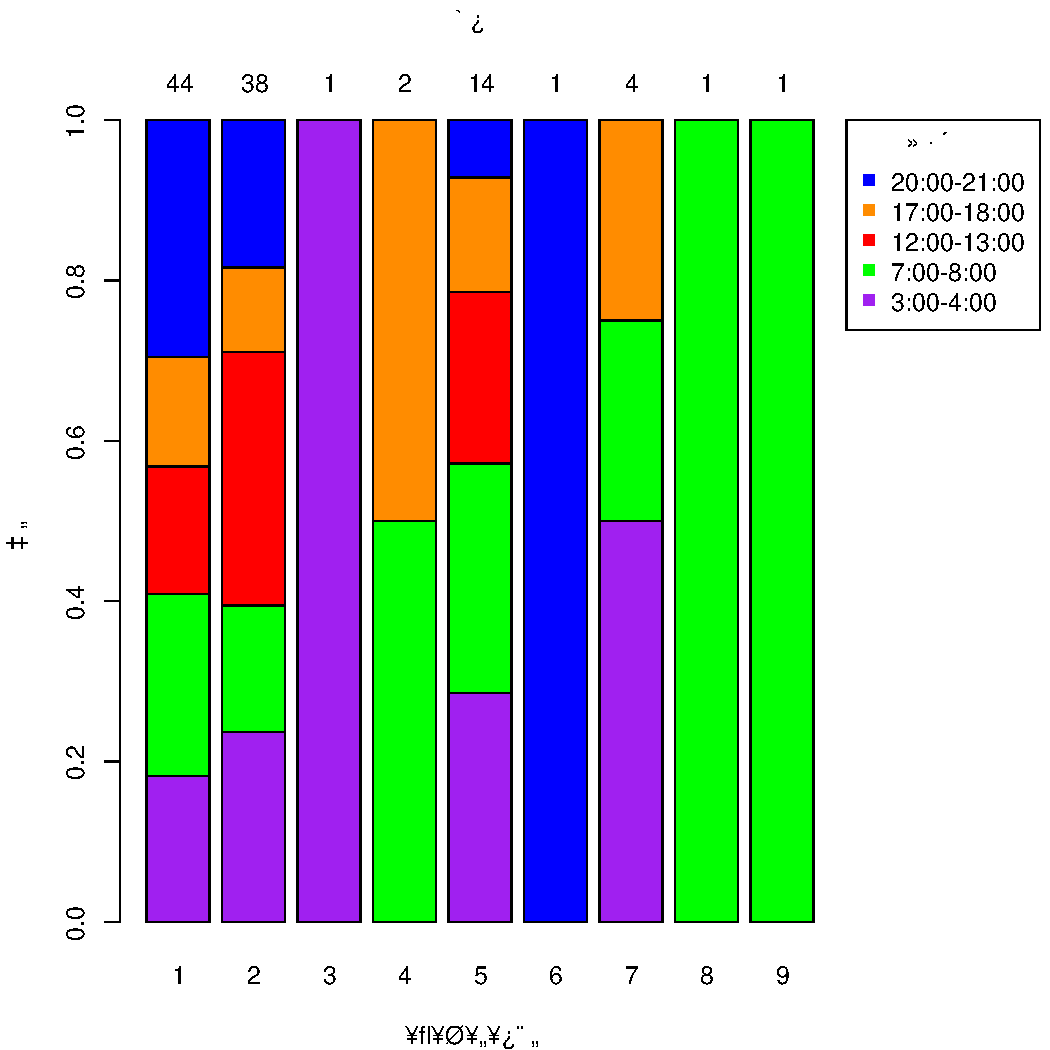
\includegraphics[height=4cm,width=6cm]{../figure/norm-manh-cent-9-timezone.pdf}
}~
\subfigure[クラスタ数 9 : 曜日]{
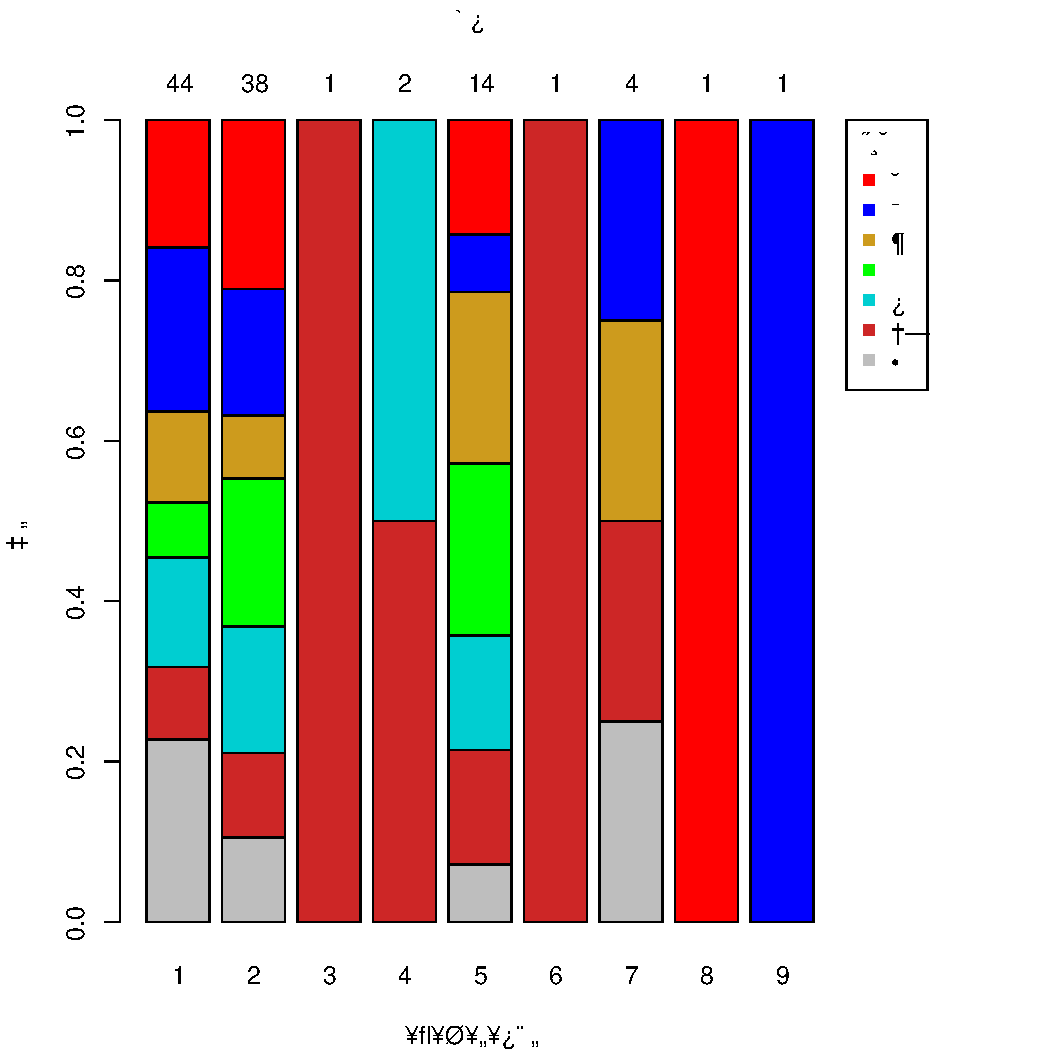
\includegraphics[height=4cm,width=6cm]{../figure/norm-manh-cent-9-day.pdf}
}\\
\subfigure[クラスタ数 12 : 時間帯]{
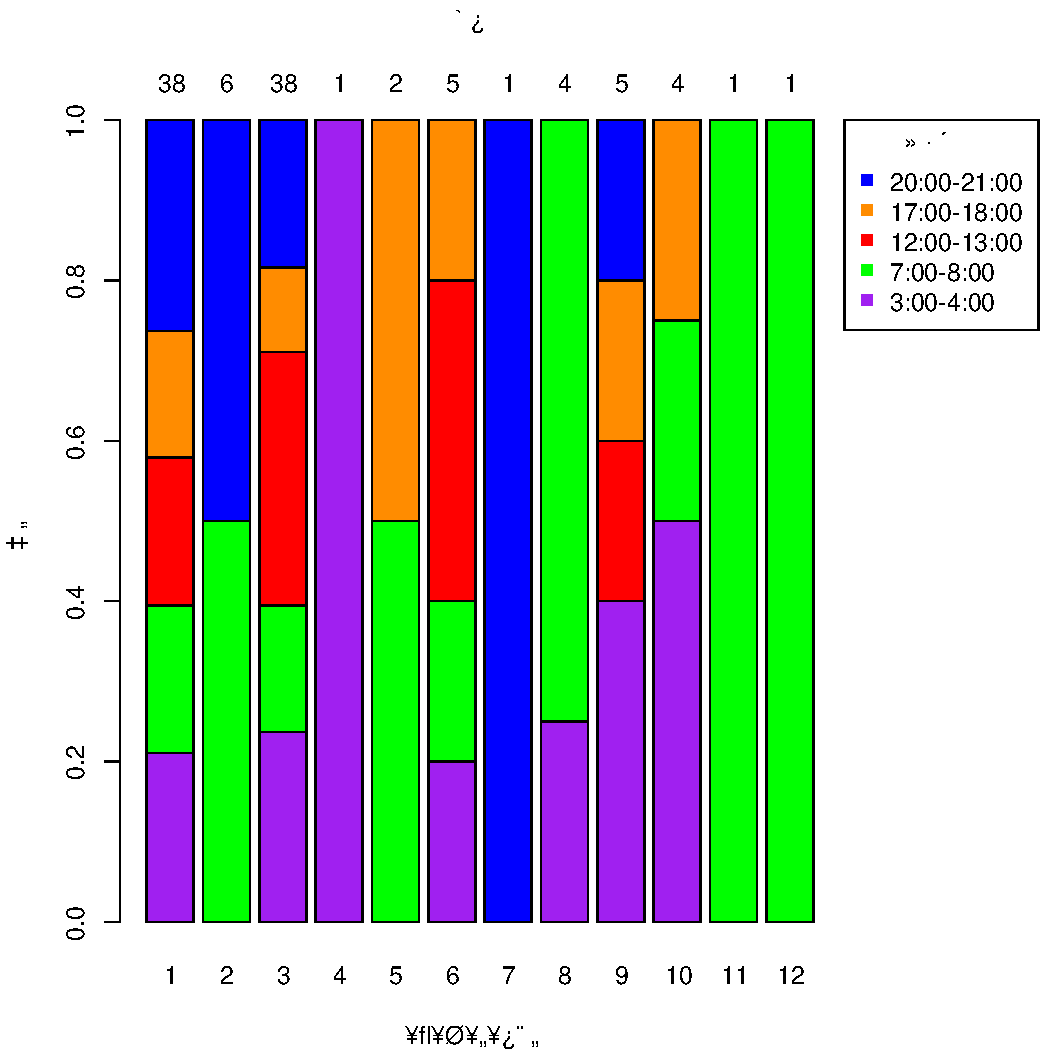
\includegraphics[height=4cm,width=6cm]{../figure/norm-manh-cent-12-timezone.pdf}
}~
\subfigure[クラスタ数 12 : 曜日]{
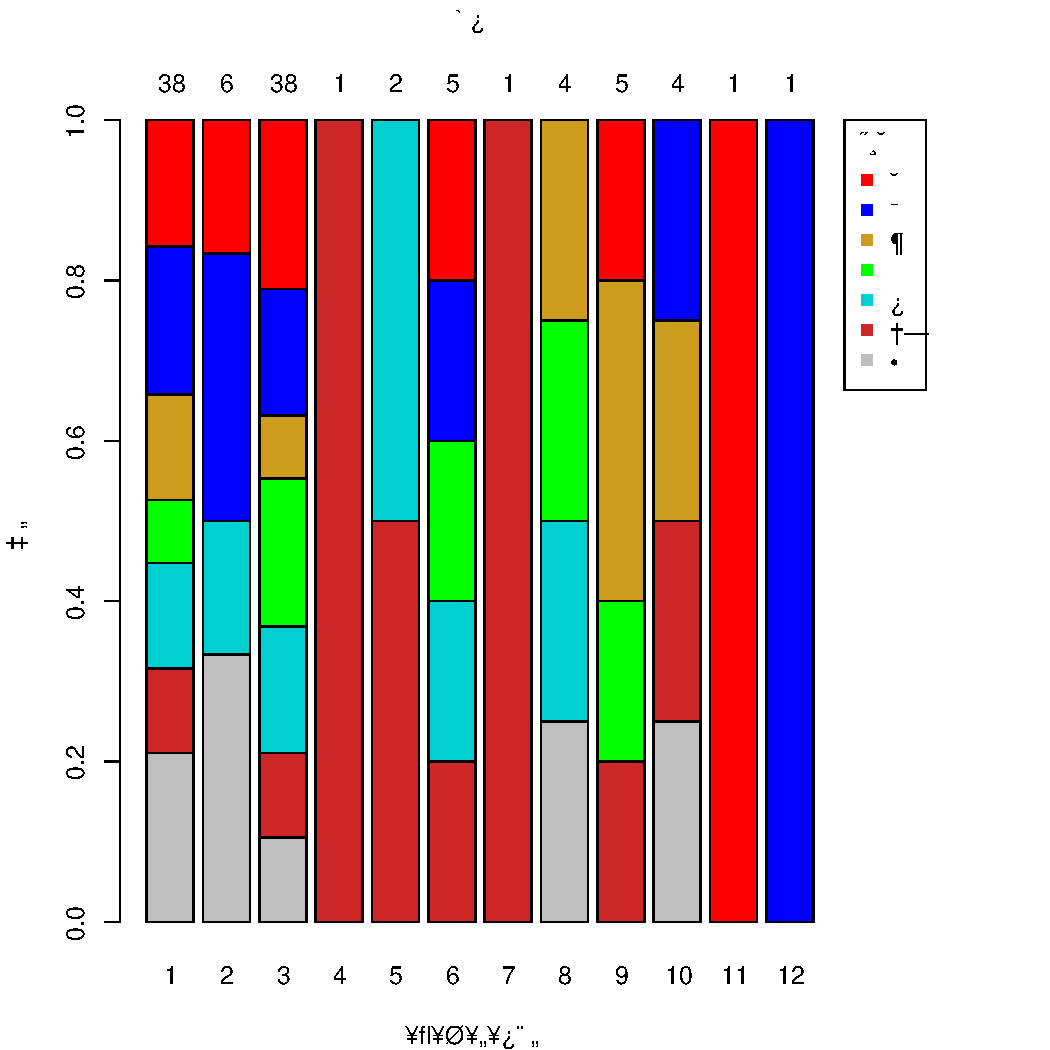
\includegraphics[height=4cm,width=6cm]{../figure/norm-manh-cent-12-day.pdf}
}\\
\subfigure[クラスタ数 15 : 時間帯]{
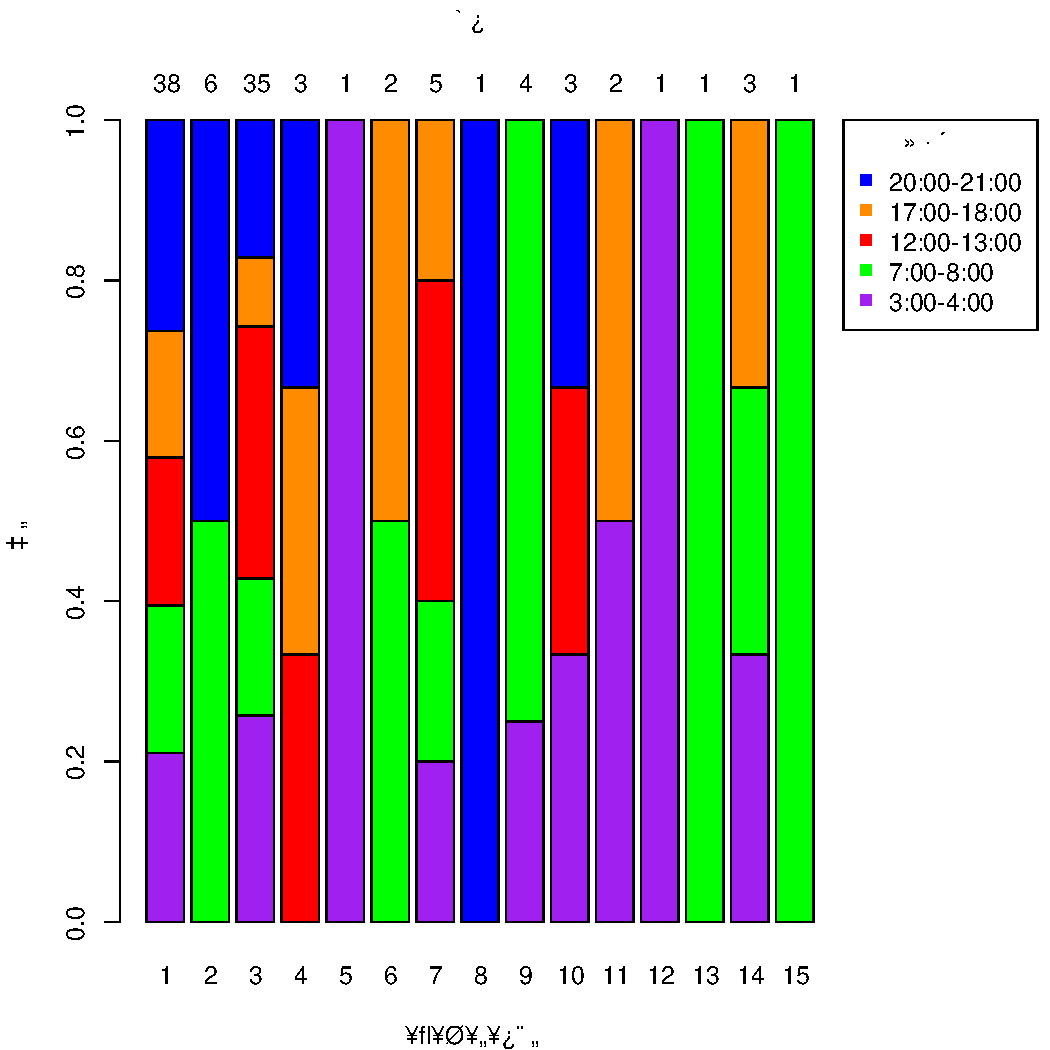
\includegraphics[height=4cm,width=6cm]{../figure/norm-manh-cent-15-timezone.pdf}
}~
\subfigure[クラスタ数 15 : 曜日]{
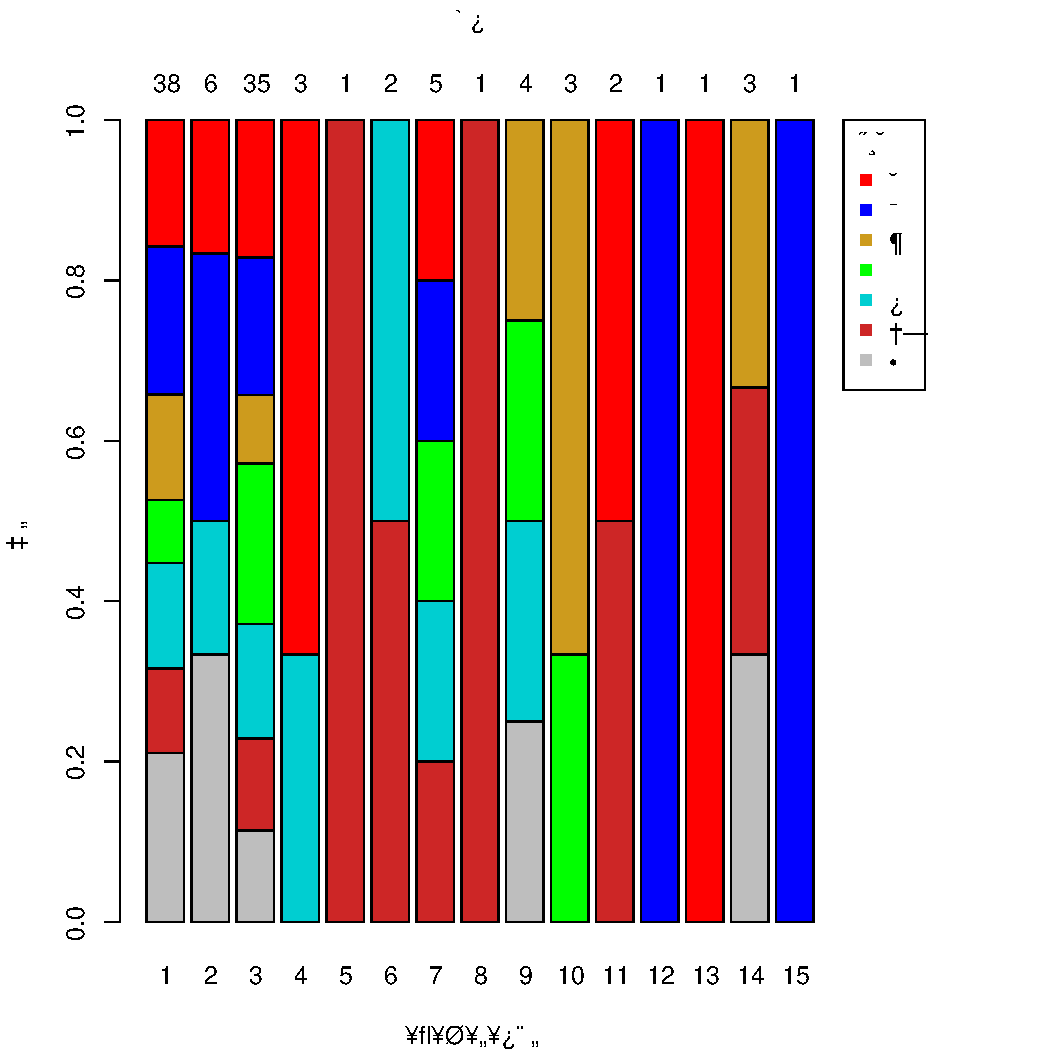
\includegraphics[height=4cm,width=6cm]{../figure/norm-manh-cent-15-day.pdf}
}\\
\caption{実測値データに対する,マンハッタン距離と重心法によるクラスタリング}
\end{center}
\end{figure}
\begin{figure}[tb]
\begin{center}
\subfigure[クラスタ数 6 : 時間帯]{
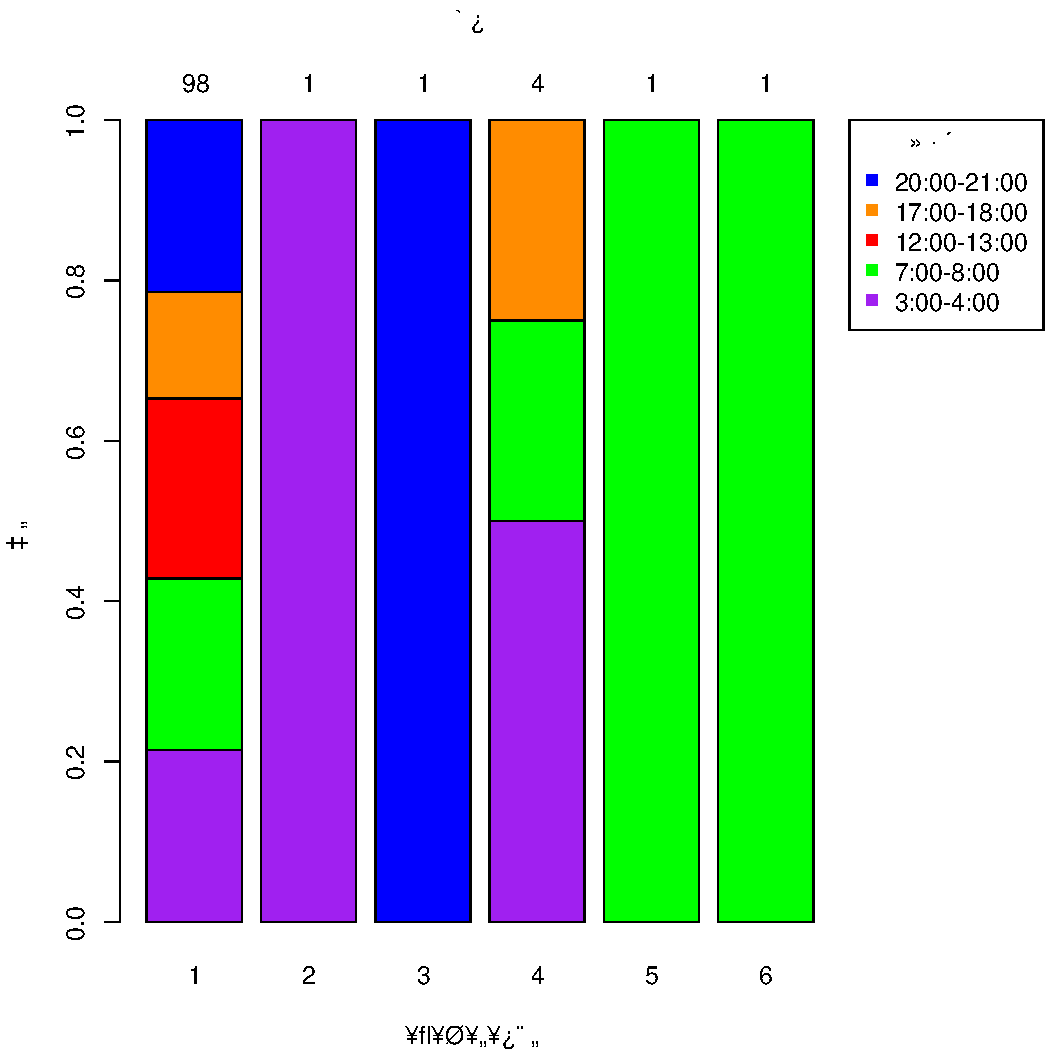
\includegraphics[height=4cm,width=6cm]{../figure/norm-manh-sing-6-timezone.pdf}
}~
\subfigure[クラスタ数 6 : 曜日]{
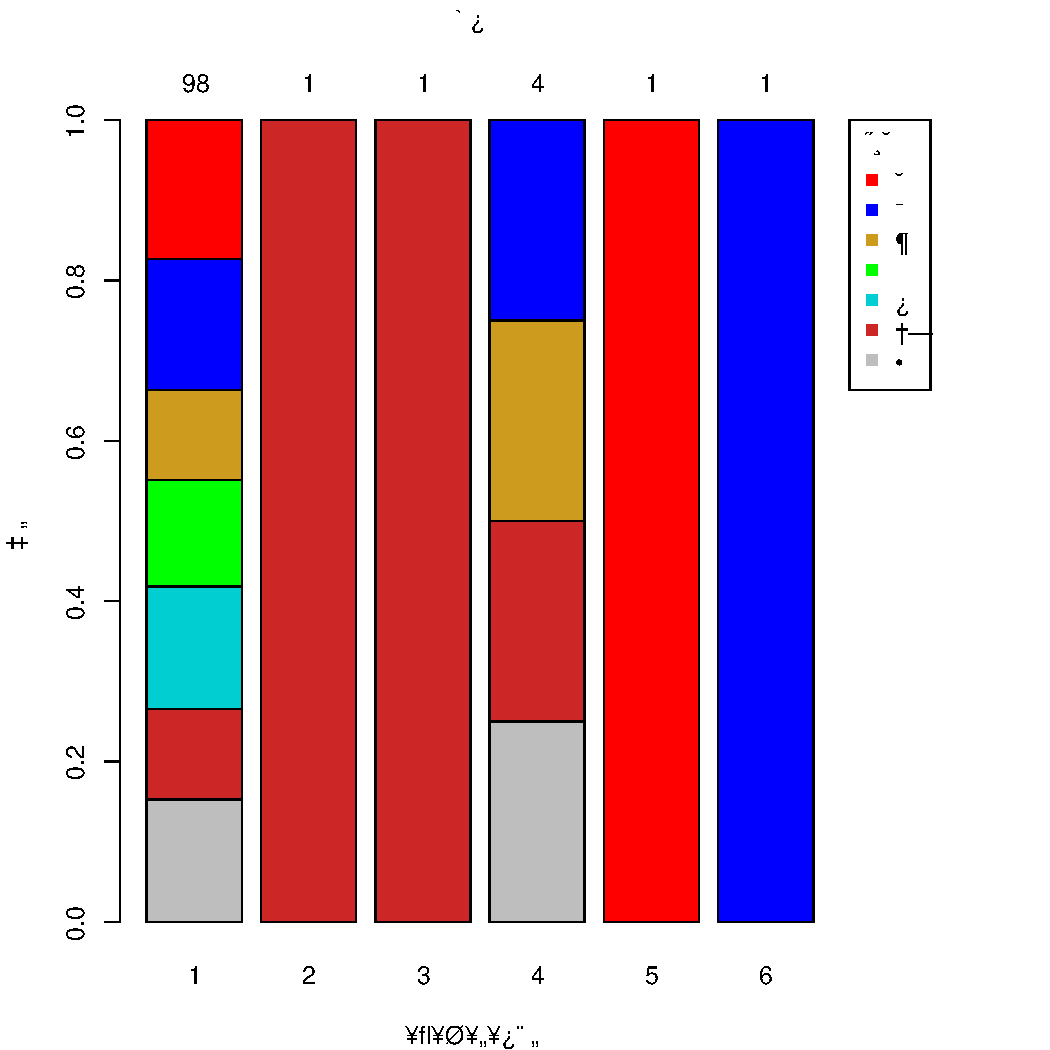
\includegraphics[height=4cm,width=6cm]{../figure/norm-manh-sing-6-day.pdf}
}\\
\subfigure[クラスタ数 7 : 時間帯]{
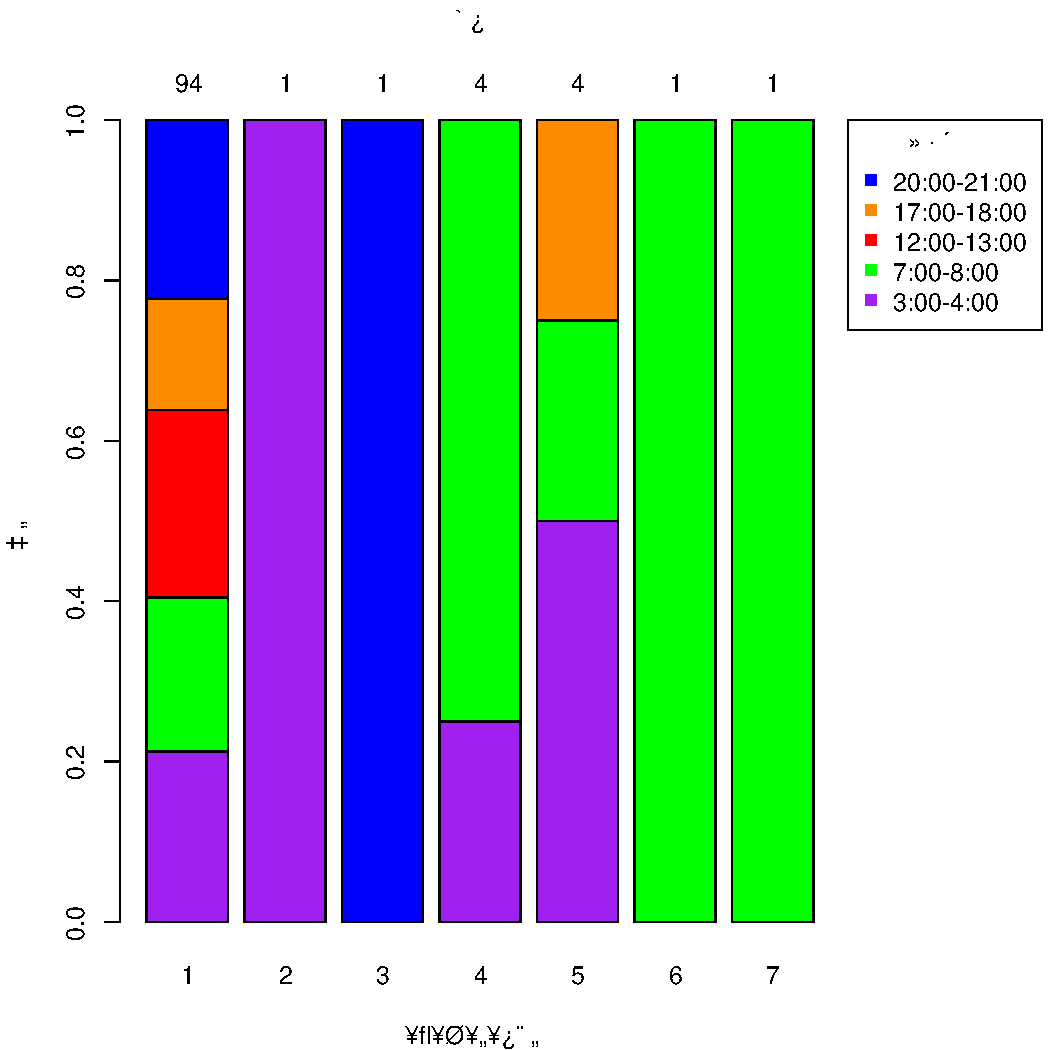
\includegraphics[height=4cm,width=6cm]{../figure/norm-manh-sing-7-timezone.pdf}
}~
\subfigure[クラスタ数 7 : 曜日]{
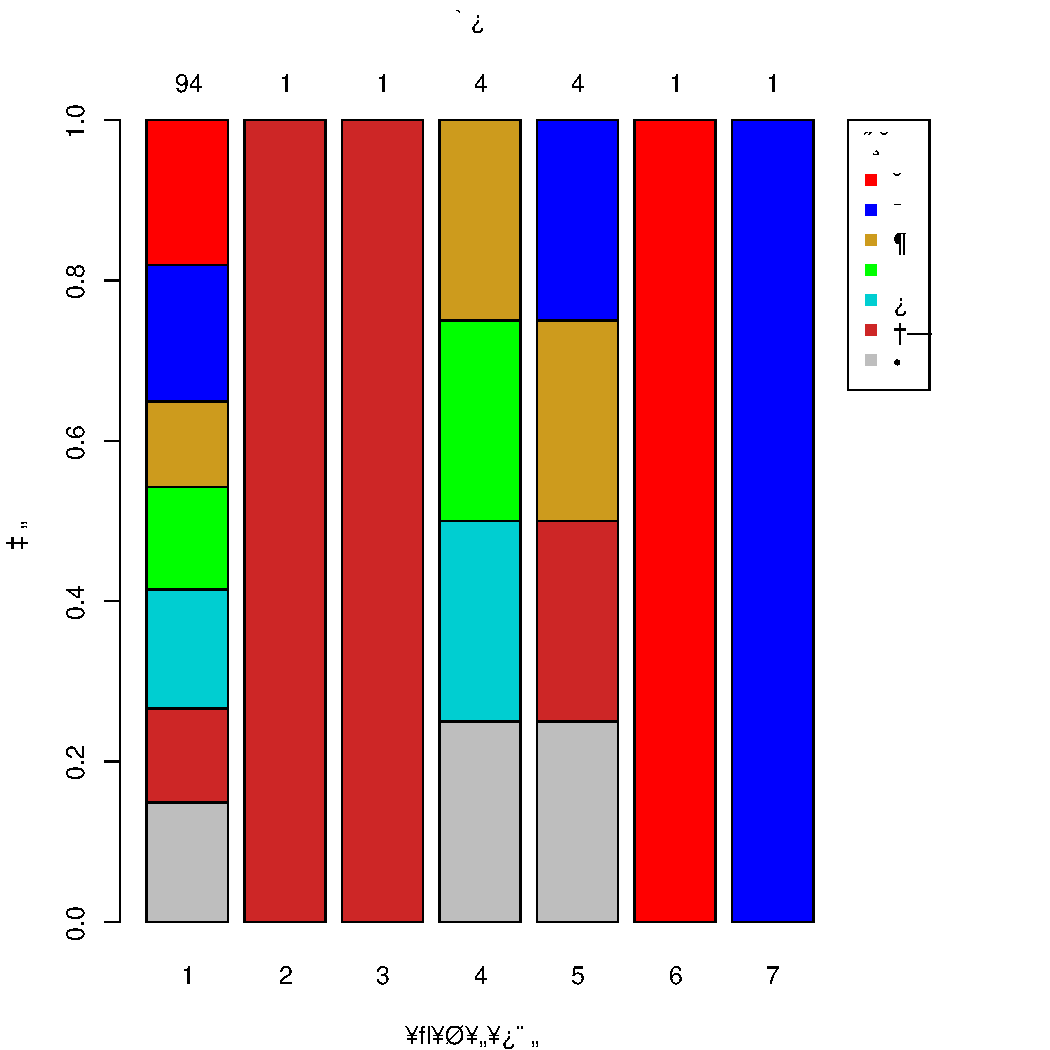
\includegraphics[height=4cm,width=6cm]{../figure/norm-manh-sing-7-day.pdf}
}\\
\subfigure[クラスタ数 9 : 時間帯]{
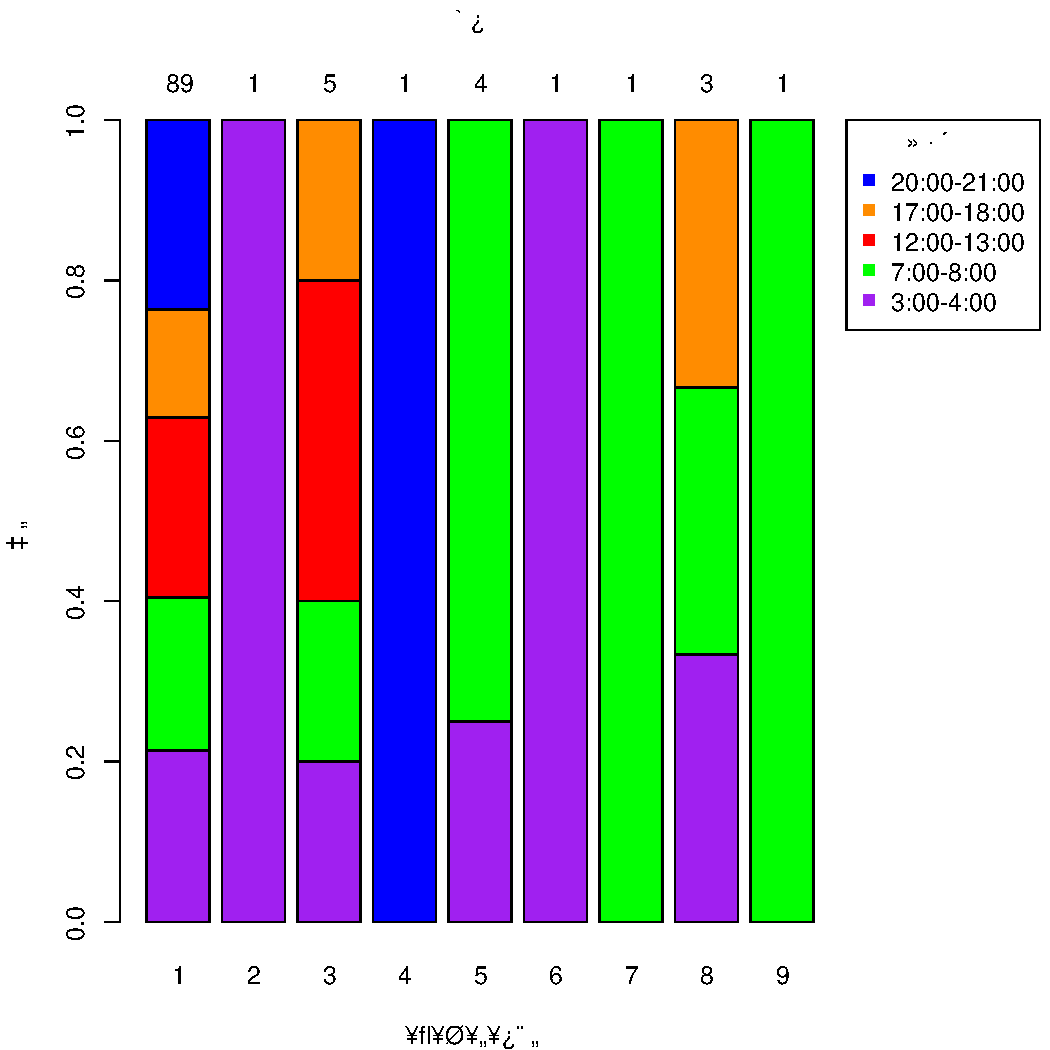
\includegraphics[height=4cm,width=6cm]{../figure/norm-manh-sing-9-timezone.pdf}
}~
\subfigure[クラスタ数 9 : 曜日]{
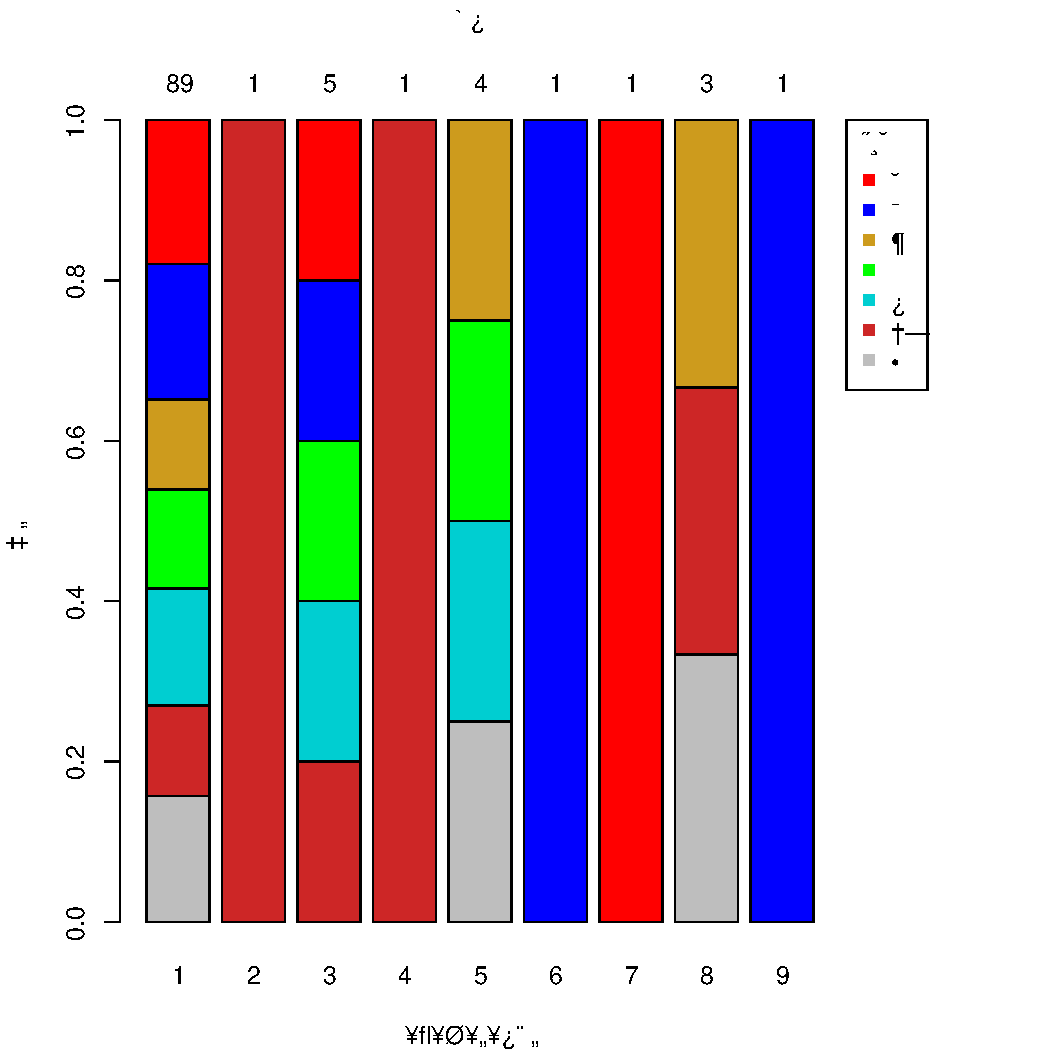
\includegraphics[height=4cm,width=6cm]{../figure/norm-manh-sing-9-day.pdf}
}\\
\subfigure[クラスタ数 12 : 時間帯]{
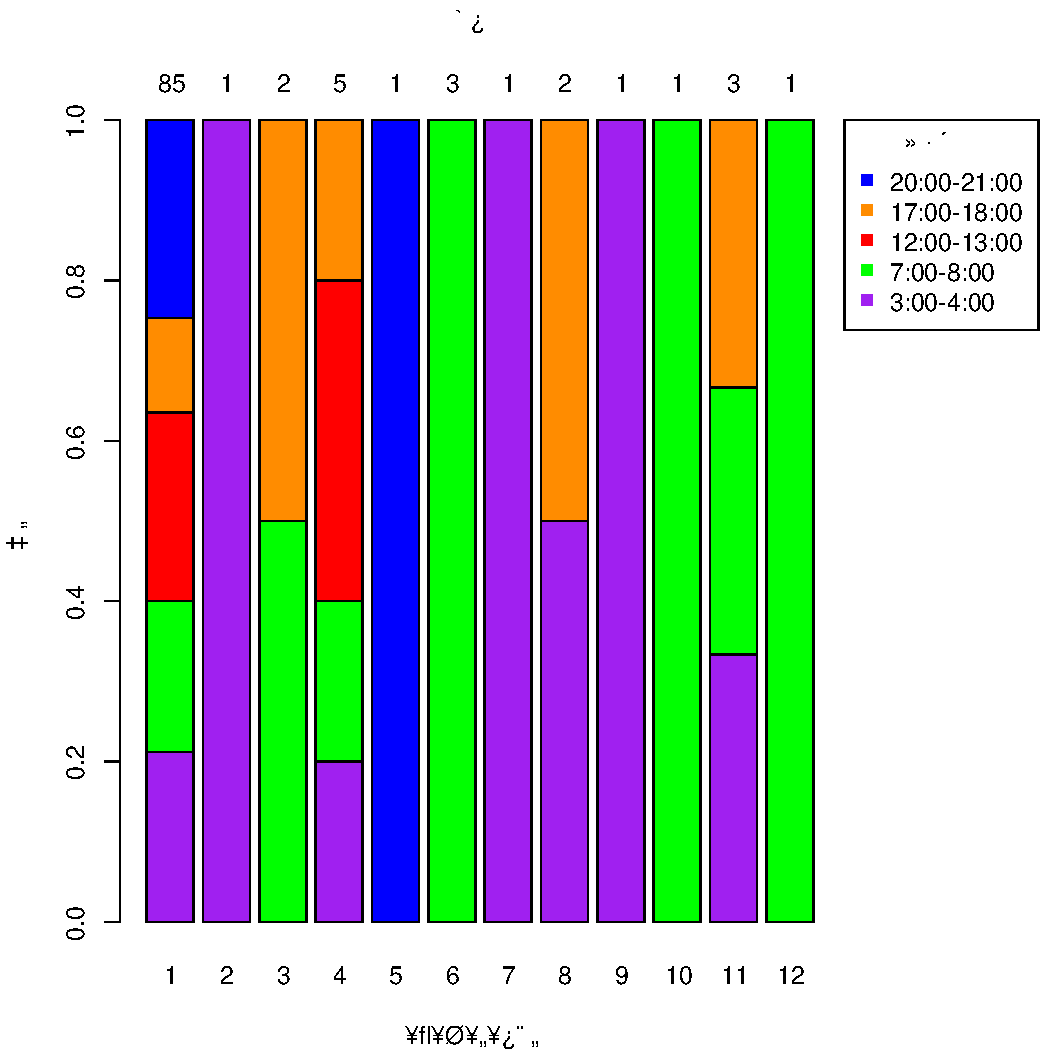
\includegraphics[height=4cm,width=6cm]{../figure/norm-manh-sing-12-timezone.pdf}
}~
\subfigure[クラスタ数 12 : 曜日]{
\includegraphics[height=4cm,width=6cm]{../figure/norm-manh-sing-12-day.pdf}
}\\
\subfigure[クラスタ数 15 : 時間帯]{
\includegraphics[height=4cm,width=6cm]{../figure/norm-manh-sing-15-timezone.pdf}
}~
\subfigure[クラスタ数 15 : 曜日]{
\includegraphics[height=4cm,width=6cm]{../figure/norm-manh-sing-15-day.pdf}
}\\
\caption{実測値データに対する,マンハッタン距離と最近傍法によるクラスタリング}
\end{center}
\end{figure}
\begin{figure}[tb]
\begin{center}
\subfigure[クラスタ数 6 : 時間帯]{
\includegraphics[height=4cm,width=6cm]{../figure/norm-manh-ward-6-timezone.pdf}
}~
\subfigure[クラスタ数 6 : 曜日]{
\includegraphics[height=4cm,width=6cm]{../figure/norm-manh-ward-6-day.pdf}
}\\
\subfigure[クラスタ数 7 : 時間帯]{
\includegraphics[height=4cm,width=6cm]{../figure/norm-manh-ward-7-timezone.pdf}
}~
\subfigure[クラスタ数 7 : 曜日]{
\includegraphics[height=4cm,width=6cm]{../figure/norm-manh-ward-7-day.pdf}
}\\
\subfigure[クラスタ数 9 : 時間帯]{
\includegraphics[height=4cm,width=6cm]{../figure/norm-manh-ward-9-timezone.pdf}
}~
\subfigure[クラスタ数 9 : 曜日]{
\includegraphics[height=4cm,width=6cm]{../figure/norm-manh-ward-9-day.pdf}
}\\
\subfigure[クラスタ数 12 : 時間帯]{
\includegraphics[height=4cm,width=6cm]{../figure/norm-manh-ward-12-timezone.pdf}
}~
\subfigure[クラスタ数 12 : 曜日]{
\includegraphics[height=4cm,width=6cm]{../figure/norm-manh-ward-12-day.pdf}
}\\
\subfigure[クラスタ数 15 : 時間帯]{
\includegraphics[height=4cm,width=6cm]{../figure/norm-manh-ward-15-timezone.pdf}
}~
\subfigure[クラスタ数 15 : 曜日]{
\includegraphics[height=4cm,width=6cm]{../figure/norm-manh-ward-15-day.pdf}
}\\
\caption{実測値データに対する,マンハッタン距離とウォード法によるクラスタリング}
\end{center}
\end{figure}
\begin{figure}[tb]
\begin{center}
\subfigure[クラスタ数 6 : 時間帯]{
\includegraphics[height=4cm,width=6cm]{../figure/norm-canb-cent-6-timezone.pdf}
}~
\subfigure[クラスタ数 6 : 曜日]{
\includegraphics[height=4cm,width=6cm]{../figure/norm-canb-cent-6-day.pdf}
}\\
\subfigure[クラスタ数 7 : 時間帯]{
\includegraphics[height=4cm,width=6cm]{../figure/norm-canb-cent-7-timezone.pdf}
}~
\subfigure[クラスタ数 7 : 曜日]{
\includegraphics[height=4cm,width=6cm]{../figure/norm-canb-cent-7-day.pdf}
}\\
\subfigure[クラスタ数 9 : 時間帯]{
\includegraphics[height=4cm,width=6cm]{../figure/norm-canb-cent-9-timezone.pdf}
}~
\subfigure[クラスタ数 9 : 曜日]{
\includegraphics[height=4cm,width=6cm]{../figure/norm-canb-cent-9-day.pdf}
}\\
\subfigure[クラスタ数 12 : 時間帯]{
\includegraphics[height=4cm,width=6cm]{../figure/norm-canb-cent-12-timezone.pdf}
}~
\subfigure[クラスタ数 12 : 曜日]{
\includegraphics[height=4cm,width=6cm]{../figure/norm-canb-cent-12-day.pdf}
}\\
\subfigure[クラスタ数 15 : 時間帯]{
\includegraphics[height=4cm,width=6cm]{../figure/norm-canb-cent-15-timezone.pdf}
}~
\subfigure[クラスタ数 15 : 曜日]{
\includegraphics[height=4cm,width=6cm]{../figure/norm-canb-cent-15-day.pdf}
}\\
\caption{実測値データに対する,キャンベラ距離と重心法によるクラスタリング}
\end{center}
\end{figure}
\begin{figure}[tb]
\begin{center}
\subfigure[クラスタ数 6 : 時間帯]{
\includegraphics[height=4cm,width=6cm]{../figure/norm-canb-sing-6-timezone.pdf}
}~
\subfigure[クラスタ数 6 : 曜日]{
\includegraphics[height=4cm,width=6cm]{../figure/norm-canb-sing-6-day.pdf}
}\\
\subfigure[クラスタ数 7 : 時間帯]{
\includegraphics[height=4cm,width=6cm]{../figure/norm-canb-sing-7-timezone.pdf}
}~
\subfigure[クラスタ数 7 : 曜日]{
\includegraphics[height=4cm,width=6cm]{../figure/norm-canb-sing-7-day.pdf}
}\\
\subfigure[クラスタ数 9 : 時間帯]{
\includegraphics[height=4cm,width=6cm]{../figure/norm-canb-sing-9-timezone.pdf}
}~
\subfigure[クラスタ数 9 : 曜日]{
\includegraphics[height=4cm,width=6cm]{../figure/norm-canb-sing-9-day.pdf}
}\\
\subfigure[クラスタ数 12 : 時間帯]{
\includegraphics[height=4cm,width=6cm]{../figure/norm-canb-sing-12-timezone.pdf}
}~
\subfigure[クラスタ数 12 : 曜日]{
\includegraphics[height=4cm,width=6cm]{../figure/norm-canb-sing-12-day.pdf}
}\\
\subfigure[クラスタ数 15 : 時間帯]{
\includegraphics[height=4cm,width=6cm]{../figure/norm-canb-sing-15-timezone.pdf}
}~
\subfigure[クラスタ数 15 : 曜日]{
\includegraphics[height=4cm,width=6cm]{../figure/norm-canb-sing-15-day.pdf}
}\\
\caption{実測値データに対する,キャンベラ距離と最近傍法によるクラスタリング}
\end{center}
\end{figure}
\begin{figure}[tb]
\begin{center}
\subfigure[クラスタ数 6 : 時間帯]{
\includegraphics[height=4cm,width=6cm]{../figure/norm-canb-ward-6-timezone.pdf}
}~
\subfigure[クラスタ数 6 : 曜日]{
\includegraphics[height=4cm,width=6cm]{../figure/norm-canb-ward-6-day.pdf}
}\\
\subfigure[クラスタ数 7 : 時間帯]{
\includegraphics[height=4cm,width=6cm]{../figure/norm-canb-ward-7-timezone.pdf}
}~
\subfigure[クラスタ数 7 : 曜日]{
\includegraphics[height=4cm,width=6cm]{../figure/norm-canb-ward-7-day.pdf}
}\\
\subfigure[クラスタ数 9 : 時間帯]{
\includegraphics[height=4cm,width=6cm]{../figure/norm-canb-ward-9-timezone.pdf}
}~
\subfigure[クラスタ数 9 : 曜日]{
\includegraphics[height=4cm,width=6cm]{../figure/norm-canb-ward-9-day.pdf}
}\\
\subfigure[クラスタ数 12 : 時間帯]{
\includegraphics[height=4cm,width=6cm]{../figure/norm-canb-ward-12-timezone.pdf}
}~
\subfigure[クラスタ数 12 : 曜日]{
\includegraphics[height=4cm,width=6cm]{../figure/norm-canb-ward-12-day.pdf}
}\\
\subfigure[クラスタ数 15 : 時間帯]{
\includegraphics[height=4cm,width=6cm]{../figure/norm-canb-ward-15-timezone.pdf}
}~
\subfigure[クラスタ数 15 : 曜日]{
\includegraphics[height=4cm,width=6cm]{../figure/norm-canb-ward-15-day.pdf}
}\\
\caption{実測値データに対する,キャンベラ距離とウォード法によるクラスタリング}
\end{center}
\end{figure}
\begin{figure}[tb]
\begin{center}
\subfigure[クラスタ数 6 : 時間帯]{
\includegraphics[height=4cm,width=6cm]{../figure/norm-eucl-kmean-6-timezone.pdf}
}~
\subfigure[クラスタ数 6 : 曜日]{
\includegraphics[height=4cm,width=6cm]{../figure/norm-eucl-kmean-6-day.pdf}
}\\
\subfigure[クラスタ数 7 : 時間帯]{
\includegraphics[height=4cm,width=6cm]{../figure/norm-eucl-kmean-7-timezone.pdf}
}~
\subfigure[クラスタ数 7 : 曜日]{
\includegraphics[height=4cm,width=6cm]{../figure/norm-eucl-kmean-7-day.pdf}
}\\
\subfigure[クラスタ数 9 : 時間帯]{
\includegraphics[height=4cm,width=6cm]{../figure/norm-eucl-kmean-9-timezone.pdf}
}~
\subfigure[クラスタ数 9 : 曜日]{
\includegraphics[height=4cm,width=6cm]{../figure/norm-eucl-kmean-9-day.pdf}
}\\
\subfigure[クラスタ数 12 : 時間帯]{
\includegraphics[height=4cm,width=6cm]{../figure/norm-eucl-kmean-12-timezone.pdf}
}~
\subfigure[クラスタ数 12 : 曜日]{
\includegraphics[height=4cm,width=6cm]{../figure/norm-eucl-kmean-12-day.pdf}
}\\
\subfigure[クラスタ数 15 : 時間帯]{
\includegraphics[height=4cm,width=6cm]{../figure/norm-eucl-kmean-15-timezone.pdf}
}~
\subfigure[クラスタ数 15 : 曜日]{
\includegraphics[height=4cm,width=6cm]{../figure/norm-eucl-kmean-15-day.pdf}
}\\
\caption{実測値データに対する,k 平均法によるクラスタリング}
\end{center}
\end{figure}



\begin{figure}[tb]
\begin{center}
\subfigure[クラスタ数 6 : 時間帯]{
\includegraphics[height=4cm,width=6cm]{../figure/diff-eucl-cent-6-timezone.pdf}
}~
\subfigure[クラスタ数 6 : 曜日]{
\includegraphics[height=4cm,width=6cm]{../figure/diff-eucl-cent-6-day.pdf}
}\\
\subfigure[クラスタ数 7 : 時間帯]{
\includegraphics[height=4cm,width=6cm]{../figure/diff-eucl-cent-7-timezone.pdf}
}~
\subfigure[クラスタ数 7 : 曜日]{
\includegraphics[height=4cm,width=6cm]{../figure/diff-eucl-cent-7-day.pdf}
}\\
\subfigure[クラスタ数 9 : 時間帯]{
\includegraphics[height=4cm,width=6cm]{../figure/diff-eucl-cent-9-timezone.pdf}
}~
\subfigure[クラスタ数 9 : 曜日]{
\includegraphics[height=4cm,width=6cm]{../figure/diff-eucl-cent-9-day.pdf}
}\\
\subfigure[クラスタ数 12 : 時間帯]{
\includegraphics[height=4cm,width=6cm]{../figure/diff-eucl-cent-12-timezone.pdf}
}~
\subfigure[クラスタ数 12 : 曜日]{
\includegraphics[height=4cm,width=6cm]{../figure/diff-eucl-cent-12-day.pdf}
}\\
\subfigure[クラスタ数 15 : 時間帯]{
\includegraphics[height=4cm,width=6cm]{../figure/diff-eucl-cent-15-timezone.pdf}
}~
\subfigure[クラスタ数 15 : 曜日]{
\includegraphics[height=4cm,width=6cm]{../figure/diff-eucl-cent-15-day.pdf}
}\\
\caption{変動値データに対する,ユークリッド距離と重心法によるクラスタリング}
\end{center}
\end{figure}
\begin{figure}[tb]
\begin{center}
\subfigure[クラスタ数 6 : 時間帯]{
\includegraphics[height=4cm,width=6cm]{../figure/diff-eucl-sing-6-timezone.pdf}
}~
\subfigure[クラスタ数 6 : 曜日]{
\includegraphics[height=4cm,width=6cm]{../figure/diff-eucl-sing-6-day.pdf}
}\\
\subfigure[クラスタ数 7 : 時間帯]{
\includegraphics[height=4cm,width=6cm]{../figure/diff-eucl-sing-7-timezone.pdf}
}~
\subfigure[クラスタ数 7 : 曜日]{
\includegraphics[height=4cm,width=6cm]{../figure/diff-eucl-sing-7-day.pdf}
}\\
\subfigure[クラスタ数 9 : 時間帯]{
\includegraphics[height=4cm,width=6cm]{../figure/diff-eucl-sing-9-timezone.pdf}
}~
\subfigure[クラスタ数 9 : 曜日]{
\includegraphics[height=4cm,width=6cm]{../figure/diff-eucl-sing-9-day.pdf}
}\\
\subfigure[クラスタ数 12 : 時間帯]{
\includegraphics[height=4cm,width=6cm]{../figure/diff-eucl-sing-12-timezone.pdf}
}~
\subfigure[クラスタ数 12 : 曜日]{
\includegraphics[height=4cm,width=6cm]{../figure/diff-eucl-sing-12-day.pdf}
}\\
\subfigure[クラスタ数 15 : 時間帯]{
\includegraphics[height=4cm,width=6cm]{../figure/diff-eucl-sing-15-timezone.pdf}
}~
\subfigure[クラスタ数 15 : 曜日]{
\includegraphics[height=4cm,width=6cm]{../figure/diff-eucl-sing-15-day.pdf}
}\\
\caption{変動値データに対する,ユークリッド距離と最近傍法によるクラスタリング}
\end{center}
\end{figure}
\begin{figure}[tb]
\begin{center}
\subfigure[クラスタ数 6 : 時間帯]{
\includegraphics[height=4cm,width=6cm]{../figure/diff-eucl-ward-6-timezone.pdf}
}~
\subfigure[クラスタ数 6 : 曜日]{
\includegraphics[height=4cm,width=6cm]{../figure/diff-eucl-ward-6-day.pdf}
}\\
\subfigure[クラスタ数 7 : 時間帯]{
\includegraphics[height=4cm,width=6cm]{../figure/diff-eucl-ward-7-timezone.pdf}
}~
\subfigure[クラスタ数 7 : 曜日]{
\includegraphics[height=4cm,width=6cm]{../figure/diff-eucl-ward-7-day.pdf}
}\\
\subfigure[クラスタ数 9 : 時間帯]{
\includegraphics[height=4cm,width=6cm]{../figure/diff-eucl-ward-9-timezone.pdf}
}~
\subfigure[クラスタ数 9 : 曜日]{
\includegraphics[height=4cm,width=6cm]{../figure/diff-eucl-ward-9-day.pdf}
}\\
\subfigure[クラスタ数 12 : 時間帯]{
\includegraphics[height=4cm,width=6cm]{../figure/diff-eucl-ward-12-timezone.pdf}
}~
\subfigure[クラスタ数 12 : 曜日]{
\includegraphics[height=4cm,width=6cm]{../figure/diff-eucl-ward-12-day.pdf}
}\\
\subfigure[クラスタ数 15 : 時間帯]{
\includegraphics[height=4cm,width=6cm]{../figure/diff-eucl-ward-15-timezone.pdf}
}~
\subfigure[クラスタ数 15 : 曜日]{
\includegraphics[height=4cm,width=6cm]{../figure/diff-eucl-ward-15-day.pdf}
}\\
\caption{変動値データに対する,ユークリッド距離とウォード法によるクラスタリング}
\end{center}
\end{figure}
\begin{figure}[tb]
\begin{center}
\subfigure[クラスタ数 6 : 時間帯]{
\includegraphics[height=4cm,width=6cm]{../figure/diff-manh-cent-6-timezone.pdf}
}~
\subfigure[クラスタ数 6 : 曜日]{
\includegraphics[height=4cm,width=6cm]{../figure/diff-manh-cent-6-day.pdf}
}\\
\subfigure[クラスタ数 7 : 時間帯]{
\includegraphics[height=4cm,width=6cm]{../figure/diff-manh-cent-7-timezone.pdf}
}~
\subfigure[クラスタ数 7 : 曜日]{
\includegraphics[height=4cm,width=6cm]{../figure/diff-manh-cent-7-day.pdf}
}\\
\subfigure[クラスタ数 9 : 時間帯]{
\includegraphics[height=4cm,width=6cm]{../figure/diff-manh-cent-9-timezone.pdf}
}~
\subfigure[クラスタ数 9 : 曜日]{
\includegraphics[height=4cm,width=6cm]{../figure/diff-manh-cent-9-day.pdf}
}\\
\subfigure[クラスタ数 12 : 時間帯]{
\includegraphics[height=4cm,width=6cm]{../figure/diff-manh-cent-12-timezone.pdf}
}~
\subfigure[クラスタ数 12 : 曜日]{
\includegraphics[height=4cm,width=6cm]{../figure/diff-manh-cent-12-day.pdf}
}\\
\subfigure[クラスタ数 15 : 時間帯]{
\includegraphics[height=4cm,width=6cm]{../figure/diff-manh-cent-15-timezone.pdf}
}~
\subfigure[クラスタ数 15 : 曜日]{
\includegraphics[height=4cm,width=6cm]{../figure/diff-manh-cent-15-day.pdf}
}\\
\caption{変動値データに対する,マンハッタン距離と重心法によるクラスタリング}
\end{center}
\end{figure}
\begin{figure}[tb]
\begin{center}
\subfigure[クラスタ数 6 : 時間帯]{
\includegraphics[height=4cm,width=6cm]{../figure/diff-manh-sing-6-timezone.pdf}
}~
\subfigure[クラスタ数 6 : 曜日]{
\includegraphics[height=4cm,width=6cm]{../figure/diff-manh-sing-6-day.pdf}
}\\
\subfigure[クラスタ数 7 : 時間帯]{
\includegraphics[height=4cm,width=6cm]{../figure/diff-manh-sing-7-timezone.pdf}
}~
\subfigure[クラスタ数 7 : 曜日]{
\includegraphics[height=4cm,width=6cm]{../figure/diff-manh-sing-7-day.pdf}
}\\
\subfigure[クラスタ数 9 : 時間帯]{
\includegraphics[height=4cm,width=6cm]{../figure/diff-manh-sing-9-timezone.pdf}
}~
\subfigure[クラスタ数 9 : 曜日]{
\includegraphics[height=4cm,width=6cm]{../figure/diff-manh-sing-9-day.pdf}
}\\
\subfigure[クラスタ数 12 : 時間帯]{
\includegraphics[height=4cm,width=6cm]{../figure/diff-manh-sing-12-timezone.pdf}
}~
\subfigure[クラスタ数 12 : 曜日]{
\includegraphics[height=4cm,width=6cm]{../figure/diff-manh-sing-12-day.pdf}
}\\
\subfigure[クラスタ数 15 : 時間帯]{
\includegraphics[height=4cm,width=6cm]{../figure/diff-manh-sing-15-timezone.pdf}
}~
\subfigure[クラスタ数 15 : 曜日]{
\includegraphics[height=4cm,width=6cm]{../figure/diff-manh-sing-15-day.pdf}
}\\
\caption{変動値データに対する,マンハッタン距離と最近傍法によるクラスタリング}
\end{center}
\end{figure}
\begin{figure}[tb]
\begin{center}
\subfigure[クラスタ数 6 : 時間帯]{
\includegraphics[height=4cm,width=6cm]{../figure/diff-manh-ward-6-timezone.pdf}
}~
\subfigure[クラスタ数 6 : 曜日]{
\includegraphics[height=4cm,width=6cm]{../figure/diff-manh-ward-6-day.pdf}
}\\
\subfigure[クラスタ数 7 : 時間帯]{
\includegraphics[height=4cm,width=6cm]{../figure/diff-manh-ward-7-timezone.pdf}
}~
\subfigure[クラスタ数 7 : 曜日]{
\includegraphics[height=4cm,width=6cm]{../figure/diff-manh-ward-7-day.pdf}
}\\
\subfigure[クラスタ数 9 : 時間帯]{
\includegraphics[height=4cm,width=6cm]{../figure/diff-manh-ward-9-timezone.pdf}
}~
\subfigure[クラスタ数 9 : 曜日]{
\includegraphics[height=4cm,width=6cm]{../figure/diff-manh-ward-9-day.pdf}
}\\
\subfigure[クラスタ数 12 : 時間帯]{
\includegraphics[height=4cm,width=6cm]{../figure/diff-manh-ward-12-timezone.pdf}
}~
\subfigure[クラスタ数 12 : 曜日]{
\includegraphics[height=4cm,width=6cm]{../figure/diff-manh-ward-12-day.pdf}
}\\
\subfigure[クラスタ数 15 : 時間帯]{
\includegraphics[height=4cm,width=6cm]{../figure/diff-manh-ward-15-timezone.pdf}
}~
\subfigure[クラスタ数 15 : 曜日]{
\includegraphics[height=4cm,width=6cm]{../figure/diff-manh-ward-15-day.pdf}
}\\
\caption{変動値データに対する,マンハッタン距離とウォード法によるクラスタリング}
\end{center}
\end{figure}
\begin{figure}[tb]
\begin{center}
\subfigure[クラスタ数 6 : 時間帯]{
\includegraphics[height=4cm,width=6cm]{../figure/diff-canb-cent-6-timezone.pdf}
}~
\subfigure[クラスタ数 6 : 曜日]{
\includegraphics[height=4cm,width=6cm]{../figure/diff-canb-cent-6-day.pdf}
}\\
\subfigure[クラスタ数 7 : 時間帯]{
\includegraphics[height=4cm,width=6cm]{../figure/diff-canb-cent-7-timezone.pdf}
}~
\subfigure[クラスタ数 7 : 曜日]{
\includegraphics[height=4cm,width=6cm]{../figure/diff-canb-cent-7-day.pdf}
}\\
\subfigure[クラスタ数 9 : 時間帯]{
\includegraphics[height=4cm,width=6cm]{../figure/diff-canb-cent-9-timezone.pdf}
}~
\subfigure[クラスタ数 9 : 曜日]{
\includegraphics[height=4cm,width=6cm]{../figure/diff-canb-cent-9-day.pdf}
}\\
\subfigure[クラスタ数 12 : 時間帯]{
\includegraphics[height=4cm,width=6cm]{../figure/diff-canb-cent-12-timezone.pdf}
}~
\subfigure[クラスタ数 12 : 曜日]{
\includegraphics[height=4cm,width=6cm]{../figure/diff-canb-cent-12-day.pdf}
}\\
\subfigure[クラスタ数 15 : 時間帯]{
\includegraphics[height=4cm,width=6cm]{../figure/diff-canb-cent-15-timezone.pdf}
}~
\subfigure[クラスタ数 15 : 曜日]{
\includegraphics[height=4cm,width=6cm]{../figure/diff-canb-cent-15-day.pdf}
}\\
\caption{変動値データに対する,キャンベラ距離と重心法によるクラスタリング}
\end{center}
\end{figure}
\begin{figure}[tb]
\begin{center}
\subfigure[クラスタ数 6 : 時間帯]{
\includegraphics[height=4cm,width=6cm]{../figure/diff-canb-sing-6-timezone.pdf}
}~
\subfigure[クラスタ数 6 : 曜日]{
\includegraphics[height=4cm,width=6cm]{../figure/diff-canb-sing-6-day.pdf}
}\\
\subfigure[クラスタ数 7 : 時間帯]{
\includegraphics[height=4cm,width=6cm]{../figure/diff-canb-sing-7-timezone.pdf}
}~
\subfigure[クラスタ数 7 : 曜日]{
\includegraphics[height=4cm,width=6cm]{../figure/diff-canb-sing-7-day.pdf}
}\\
\subfigure[クラスタ数 9 : 時間帯]{
\includegraphics[height=4cm,width=6cm]{../figure/diff-canb-sing-9-timezone.pdf}
}~
\subfigure[クラスタ数 9 : 曜日]{
\includegraphics[height=4cm,width=6cm]{../figure/diff-canb-sing-9-day.pdf}
}\\
\subfigure[クラスタ数 12 : 時間帯]{
\includegraphics[height=4cm,width=6cm]{../figure/diff-canb-sing-12-timezone.pdf}
}~
\subfigure[クラスタ数 12 : 曜日]{
\includegraphics[height=4cm,width=6cm]{../figure/diff-canb-sing-12-day.pdf}
}\\
\subfigure[クラスタ数 15 : 時間帯]{
\includegraphics[height=4cm,width=6cm]{../figure/diff-canb-sing-15-timezone.pdf}
}~
\subfigure[クラスタ数 15 : 曜日]{
\includegraphics[height=4cm,width=6cm]{../figure/diff-canb-sing-15-day.pdf}
}\\
\caption{変動値データに対する,キャンベラ距離と最近傍法によるクラスタリング}
\end{center}
\end{figure}
\begin{figure}[tb]
\begin{center}
\subfigure[クラスタ数 6 : 時間帯]{
\includegraphics[height=4cm,width=6cm]{../figure/diff-canb-ward-6-timezone.pdf}
}~
\subfigure[クラスタ数 6 : 曜日]{
\includegraphics[height=4cm,width=6cm]{../figure/diff-canb-ward-6-day.pdf}
}\\
\subfigure[クラスタ数 7 : 時間帯]{
\includegraphics[height=4cm,width=6cm]{../figure/diff-canb-ward-7-timezone.pdf}
}~
\subfigure[クラスタ数 7 : 曜日]{
\includegraphics[height=4cm,width=6cm]{../figure/diff-canb-ward-7-day.pdf}
}\\
\subfigure[クラスタ数 9 : 時間帯]{
\includegraphics[height=4cm,width=6cm]{../figure/diff-canb-ward-9-timezone.pdf}
}~
\subfigure[クラスタ数 9 : 曜日]{
\includegraphics[height=4cm,width=6cm]{../figure/diff-canb-ward-9-day.pdf}
}\\
\subfigure[クラスタ数 12 : 時間帯]{
\includegraphics[height=4cm,width=6cm]{../figure/diff-canb-ward-12-timezone.pdf}
}~
\subfigure[クラスタ数 12 : 曜日]{
\includegraphics[height=4cm,width=6cm]{../figure/diff-canb-ward-12-day.pdf}
}\\
\subfigure[クラスタ数 15 : 時間帯]{
\includegraphics[height=4cm,width=6cm]{../figure/diff-canb-ward-15-timezone.pdf}
}~
\subfigure[クラスタ数 15 : 曜日]{
\includegraphics[height=4cm,width=6cm]{../figure/diff-canb-ward-15-day.pdf}
}\\
\caption{変動値データに対する,キャンベラ距離とウォード法によるクラスタリング}
\end{center}
\end{figure}
\begin{figure}[tb]
\begin{center}
\subfigure[クラスタ数 6 : 時間帯]{
\includegraphics[height=4cm,width=6cm]{../figure/diff-eucl-kmean-6-timezone.pdf}
}~
\subfigure[クラスタ数 6 : 曜日]{
\includegraphics[height=4cm,width=6cm]{../figure/diff-eucl-kmean-6-day.pdf}
}\\
\subfigure[クラスタ数 7 : 時間帯]{
\includegraphics[height=4cm,width=6cm]{../figure/diff-eucl-kmean-7-timezone.pdf}
}~
\subfigure[クラスタ数 7 : 曜日]{
\includegraphics[height=4cm,width=6cm]{../figure/diff-eucl-kmean-7-day.pdf}
}\\
\subfigure[クラスタ数 9 : 時間帯]{
\includegraphics[height=4cm,width=6cm]{../figure/diff-eucl-kmean-9-timezone.pdf}
}~
\subfigure[クラスタ数 9 : 曜日]{
\includegraphics[height=4cm,width=6cm]{../figure/diff-eucl-kmean-9-day.pdf}
}\\
\subfigure[クラスタ数 12 : 時間帯]{
\includegraphics[height=4cm,width=6cm]{../figure/diff-eucl-kmean-12-timezone.pdf}
}~
\subfigure[クラスタ数 12 : 曜日]{
\includegraphics[height=4cm,width=6cm]{../figure/diff-eucl-kmean-12-day.pdf}
}\\
\subfigure[クラスタ数 15 : 時間帯]{
\includegraphics[height=4cm,width=6cm]{../figure/diff-eucl-kmean-15-timezone.pdf}
}~
\subfigure[クラスタ数 15 : 曜日]{
\includegraphics[height=4cm,width=6cm]{../figure/diff-eucl-kmean-15-day.pdf}
}\\
\caption{変動値データに対する,k 平均法によるクラスタリング}
\label{cluster2}
\end{center}
\end{figure}





\begin{figure}[tb]
\begin{center}
\subfigure[クラスタ数 6 : 時間帯]{
\includegraphics[height=4cm,width=6cm]{../figure/norm_comp-eucl-cent-6-timezone.pdf}
}~
\subfigure[クラスタ数 6 : 曜日]{
\includegraphics[height=4cm,width=6cm]{../figure/norm_comp-eucl-cent-6-day.pdf}
}\\
\subfigure[クラスタ数 7 : 時間帯]{
\includegraphics[height=4cm,width=6cm]{../figure/norm_comp-eucl-cent-7-timezone.pdf}
}~
\subfigure[クラスタ数 7 : 曜日]{
\includegraphics[height=4cm,width=6cm]{../figure/norm_comp-eucl-cent-7-day.pdf}
}\\
\subfigure[クラスタ数 9 : 時間帯]{
\includegraphics[height=4cm,width=6cm]{../figure/norm_comp-eucl-cent-9-timezone.pdf}
}~
\subfigure[クラスタ数 9 : 曜日]{
\includegraphics[height=4cm,width=6cm]{../figure/norm_comp-eucl-cent-9-day.pdf}
}\\
\subfigure[クラスタ数 12 : 時間帯]{
\includegraphics[height=4cm,width=6cm]{../figure/norm_comp-eucl-cent-12-timezone.pdf}
}~
\subfigure[クラスタ数 12 : 曜日]{
\includegraphics[height=4cm,width=6cm]{../figure/norm_comp-eucl-cent-12-day.pdf}
}\\
\subfigure[クラスタ数 15 : 時間帯]{
\includegraphics[height=4cm,width=6cm]{../figure/norm_comp-eucl-cent-15-timezone.pdf}
}~
\subfigure[クラスタ数 15 : 曜日]{
\includegraphics[height=4cm,width=6cm]{../figure/norm_comp-eucl-cent-15-day.pdf}
}\\
\caption{実測値データの主成分に対する,ユークリッド距離と重心法によるクラスタリング}
\label{cluster3}
\end{center}
\end{figure}
\begin{figure}[tb]
\begin{center}
\subfigure[クラスタ数 6 : 時間帯]{
\includegraphics[height=4cm,width=6cm]{../figure/norm_comp-eucl-sing-6-timezone.pdf}
}~
\subfigure[クラスタ数 6 : 曜日]{
\includegraphics[height=4cm,width=6cm]{../figure/norm_comp-eucl-sing-6-day.pdf}
}\\
\subfigure[クラスタ数 7 : 時間帯]{
\includegraphics[height=4cm,width=6cm]{../figure/norm_comp-eucl-sing-7-timezone.pdf}
}~
\subfigure[クラスタ数 7 : 曜日]{
\includegraphics[height=4cm,width=6cm]{../figure/norm_comp-eucl-sing-7-day.pdf}
}\\
\subfigure[クラスタ数 9 : 時間帯]{
\includegraphics[height=4cm,width=6cm]{../figure/norm_comp-eucl-sing-9-timezone.pdf}
}~
\subfigure[クラスタ数 9 : 曜日]{
\includegraphics[height=4cm,width=6cm]{../figure/norm_comp-eucl-sing-9-day.pdf}
}\\
\subfigure[クラスタ数 12 : 時間帯]{
\includegraphics[height=4cm,width=6cm]{../figure/norm_comp-eucl-sing-12-timezone.pdf}
}~
\subfigure[クラスタ数 12 : 曜日]{
\includegraphics[height=4cm,width=6cm]{../figure/norm_comp-eucl-sing-12-day.pdf}
}\\
\subfigure[クラスタ数 15 : 時間帯]{
\includegraphics[height=4cm,width=6cm]{../figure/norm_comp-eucl-sing-15-timezone.pdf}
}~
\subfigure[クラスタ数 15 : 曜日]{
\includegraphics[height=4cm,width=6cm]{../figure/norm_comp-eucl-sing-15-day.pdf}
}\\
\caption{実測値データの主成分に対する,ユークリッド距離と最近傍法によるクラスタリング}
\end{center}
\end{figure}
\begin{figure}[tb]
\begin{center}
\subfigure[クラスタ数 6 : 時間帯]{
\includegraphics[height=4cm,width=6cm]{../figure/norm_comp-eucl-ward-6-timezone.pdf}
}~
\subfigure[クラスタ数 6 : 曜日]{
\includegraphics[height=4cm,width=6cm]{../figure/norm_comp-eucl-ward-6-day.pdf}
}\\
\subfigure[クラスタ数 7 : 時間帯]{
\includegraphics[height=4cm,width=6cm]{../figure/norm_comp-eucl-ward-7-timezone.pdf}
}~
\subfigure[クラスタ数 7 : 曜日]{
\includegraphics[height=4cm,width=6cm]{../figure/norm_comp-eucl-ward-7-day.pdf}
}\\
\subfigure[クラスタ数 9 : 時間帯]{
\includegraphics[height=4cm,width=6cm]{../figure/norm_comp-eucl-ward-9-timezone.pdf}
}~
\subfigure[クラスタ数 9 : 曜日]{
\includegraphics[height=4cm,width=6cm]{../figure/norm_comp-eucl-ward-9-day.pdf}
}\\
\subfigure[クラスタ数 12 : 時間帯]{
\includegraphics[height=4cm,width=6cm]{../figure/norm_comp-eucl-ward-12-timezone.pdf}
}~
\subfigure[クラスタ数 12 : 曜日]{
\includegraphics[height=4cm,width=6cm]{../figure/norm_comp-eucl-ward-12-day.pdf}
}\\
\subfigure[クラスタ数 15 : 時間帯]{
\includegraphics[height=4cm,width=6cm]{../figure/norm_comp-eucl-ward-15-timezone.pdf}
}~
\subfigure[クラスタ数 15 : 曜日]{
\includegraphics[height=4cm,width=6cm]{../figure/norm_comp-eucl-ward-15-day.pdf}
}\\
\caption{実測値データの主成分に対する,ユークリッド距離とウォード法によるクラスタリング}
\end{center}
\end{figure}
\begin{figure}[tb]
\begin{center}
\subfigure[クラスタ数 6 : 時間帯]{
\includegraphics[height=4cm,width=6cm]{../figure/norm_comp-manh-cent-6-timezone.pdf}
}~
\subfigure[クラスタ数 6 : 曜日]{
\includegraphics[height=4cm,width=6cm]{../figure/norm_comp-manh-cent-6-day.pdf}
}\\
\subfigure[クラスタ数 7 : 時間帯]{
\includegraphics[height=4cm,width=6cm]{../figure/norm_comp-manh-cent-7-timezone.pdf}
}~
\subfigure[クラスタ数 7 : 曜日]{
\includegraphics[height=4cm,width=6cm]{../figure/norm_comp-manh-cent-7-day.pdf}
}\\
\subfigure[クラスタ数 9 : 時間帯]{
\includegraphics[height=4cm,width=6cm]{../figure/norm_comp-manh-cent-9-timezone.pdf}
}~
\subfigure[クラスタ数 9 : 曜日]{
\includegraphics[height=4cm,width=6cm]{../figure/norm_comp-manh-cent-9-day.pdf}
}\\
\subfigure[クラスタ数 12 : 時間帯]{
\includegraphics[height=4cm,width=6cm]{../figure/norm_comp-manh-cent-12-timezone.pdf}
}~
\subfigure[クラスタ数 12 : 曜日]{
\includegraphics[height=4cm,width=6cm]{../figure/norm_comp-manh-cent-12-day.pdf}
}\\
\subfigure[クラスタ数 15 : 時間帯]{
\includegraphics[height=4cm,width=6cm]{../figure/norm_comp-manh-cent-15-timezone.pdf}
}~
\subfigure[クラスタ数 15 : 曜日]{
\includegraphics[height=4cm,width=6cm]{../figure/norm_comp-manh-cent-15-day.pdf}
}\\
\caption{実測値データの主成分に対する,マンハッタン距離と重心法によるクラスタリング}
\end{center}
\end{figure}
\begin{figure}[tb]
\begin{center}
\subfigure[クラスタ数 6 : 時間帯]{
\includegraphics[height=4cm,width=6cm]{../figure/norm_comp-manh-sing-6-timezone.pdf}
}~
\subfigure[クラスタ数 6 : 曜日]{
\includegraphics[height=4cm,width=6cm]{../figure/norm_comp-manh-sing-6-day.pdf}
}\\
\subfigure[クラスタ数 7 : 時間帯]{
\includegraphics[height=4cm,width=6cm]{../figure/norm_comp-manh-sing-7-timezone.pdf}
}~
\subfigure[クラスタ数 7 : 曜日]{
\includegraphics[height=4cm,width=6cm]{../figure/norm_comp-manh-sing-7-day.pdf}
}\\
\subfigure[クラスタ数 9 : 時間帯]{
\includegraphics[height=4cm,width=6cm]{../figure/norm_comp-manh-sing-9-timezone.pdf}
}~
\subfigure[クラスタ数 9 : 曜日]{
\includegraphics[height=4cm,width=6cm]{../figure/norm_comp-manh-sing-9-day.pdf}
}\\
\subfigure[クラスタ数 12 : 時間帯]{
\includegraphics[height=4cm,width=6cm]{../figure/norm_comp-manh-sing-12-timezone.pdf}
}~
\subfigure[クラスタ数 12 : 曜日]{
\includegraphics[height=4cm,width=6cm]{../figure/norm_comp-manh-sing-12-day.pdf}
}\\
\subfigure[クラスタ数 15 : 時間帯]{
\includegraphics[height=4cm,width=6cm]{../figure/norm_comp-manh-sing-15-timezone.pdf}
}~
\subfigure[クラスタ数 15 : 曜日]{
\includegraphics[height=4cm,width=6cm]{../figure/norm_comp-manh-sing-15-day.pdf}
}\\
\caption{実測値データの主成分に対する,マンハッタン距離と最近傍法によるクラスタリング}
\end{center}
\end{figure}
\begin{figure}[tb]
\begin{center}
\subfigure[クラスタ数 6 : 時間帯]{
\includegraphics[height=4cm,width=6cm]{../figure/norm_comp-manh-ward-6-timezone.pdf}
}~
\subfigure[クラスタ数 6 : 曜日]{
\includegraphics[height=4cm,width=6cm]{../figure/norm_comp-manh-ward-6-day.pdf}
}\\
\subfigure[クラスタ数 7 : 時間帯]{
\includegraphics[height=4cm,width=6cm]{../figure/norm_comp-manh-ward-7-timezone.pdf}
}~
\subfigure[クラスタ数 7 : 曜日]{
\includegraphics[height=4cm,width=6cm]{../figure/norm_comp-manh-ward-7-day.pdf}
}\\
\subfigure[クラスタ数 9 : 時間帯]{
\includegraphics[height=4cm,width=6cm]{../figure/norm_comp-manh-ward-9-timezone.pdf}
}~
\subfigure[クラスタ数 9 : 曜日]{
\includegraphics[height=4cm,width=6cm]{../figure/norm_comp-manh-ward-9-day.pdf}
}\\
\subfigure[クラスタ数 12 : 時間帯]{
\includegraphics[height=4cm,width=6cm]{../figure/norm_comp-manh-ward-12-timezone.pdf}
}~
\subfigure[クラスタ数 12 : 曜日]{
\includegraphics[height=4cm,width=6cm]{../figure/norm_comp-manh-ward-12-day.pdf}
}\\
\subfigure[クラスタ数 15 : 時間帯]{
\includegraphics[height=4cm,width=6cm]{../figure/norm_comp-manh-ward-15-timezone.pdf}
}~
\subfigure[クラスタ数 15 : 曜日]{
\includegraphics[height=4cm,width=6cm]{../figure/norm_comp-manh-ward-15-day.pdf}
}\\
\caption{実測値データの主成分に対する,マンハッタン距離とウォード法によるクラスタリング}
\end{center}
\end{figure}
\begin{figure}[tb]
\begin{center}
\subfigure[クラスタ数 6 : 時間帯]{
\includegraphics[height=4cm,width=6cm]{../figure/norm_comp-canb-cent-6-timezone.pdf}
}~
\subfigure[クラスタ数 6 : 曜日]{
\includegraphics[height=4cm,width=6cm]{../figure/norm_comp-canb-cent-6-day.pdf}
}\\
\subfigure[クラスタ数 7 : 時間帯]{
\includegraphics[height=4cm,width=6cm]{../figure/norm_comp-canb-cent-7-timezone.pdf}
}~
\subfigure[クラスタ数 7 : 曜日]{
\includegraphics[height=4cm,width=6cm]{../figure/norm_comp-canb-cent-7-day.pdf}
}\\
\subfigure[クラスタ数 9 : 時間帯]{
\includegraphics[height=4cm,width=6cm]{../figure/norm_comp-canb-cent-9-timezone.pdf}
}~
\subfigure[クラスタ数 9 : 曜日]{
\includegraphics[height=4cm,width=6cm]{../figure/norm_comp-canb-cent-9-day.pdf}
}\\
\subfigure[クラスタ数 12 : 時間帯]{
\includegraphics[height=4cm,width=6cm]{../figure/norm_comp-canb-cent-12-timezone.pdf}
}~
\subfigure[クラスタ数 12 : 曜日]{
\includegraphics[height=4cm,width=6cm]{../figure/norm_comp-canb-cent-12-day.pdf}
}\\
\subfigure[クラスタ数 15 : 時間帯]{
\includegraphics[height=4cm,width=6cm]{../figure/norm_comp-canb-cent-15-timezone.pdf}
}~
\subfigure[クラスタ数 15 : 曜日]{
\includegraphics[height=4cm,width=6cm]{../figure/norm_comp-canb-cent-15-day.pdf}
}\\
\caption{実測値データの主成分に対する,キャンベラ距離と重心法によるクラスタリング}
\end{center}
\end{figure}
\begin{figure}[tb]
\begin{center}
\subfigure[クラスタ数 6 : 時間帯]{
\includegraphics[height=4cm,width=6cm]{../figure/norm_comp-canb-sing-6-timezone.pdf}
}~
\subfigure[クラスタ数 6 : 曜日]{
\includegraphics[height=4cm,width=6cm]{../figure/norm_comp-canb-sing-6-day.pdf}
}\\
\subfigure[クラスタ数 7 : 時間帯]{
\includegraphics[height=4cm,width=6cm]{../figure/norm_comp-canb-sing-7-timezone.pdf}
}~
\subfigure[クラスタ数 7 : 曜日]{
\includegraphics[height=4cm,width=6cm]{../figure/norm_comp-canb-sing-7-day.pdf}
}\\
\subfigure[クラスタ数 9 : 時間帯]{
\includegraphics[height=4cm,width=6cm]{../figure/norm_comp-canb-sing-9-timezone.pdf}
}~
\subfigure[クラスタ数 9 : 曜日]{
\includegraphics[height=4cm,width=6cm]{../figure/norm_comp-canb-sing-9-day.pdf}
}\\
\subfigure[クラスタ数 12 : 時間帯]{
\includegraphics[height=4cm,width=6cm]{../figure/norm_comp-canb-sing-12-timezone.pdf}
}~
\subfigure[クラスタ数 12 : 曜日]{
\includegraphics[height=4cm,width=6cm]{../figure/norm_comp-canb-sing-12-day.pdf}
}\\
\subfigure[クラスタ数 15 : 時間帯]{
\includegraphics[height=4cm,width=6cm]{../figure/norm_comp-canb-sing-15-timezone.pdf}
}~
\subfigure[クラスタ数 15 : 曜日]{
\includegraphics[height=4cm,width=6cm]{../figure/norm_comp-canb-sing-15-day.pdf}
}\\
\caption{実測値データの主成分に対する,キャンベラ距離と最近傍法によるクラスタリング}
\end{center}
\end{figure}
\begin{figure}[tb]
\begin{center}
\subfigure[クラスタ数 6 : 時間帯]{
\includegraphics[height=4cm,width=6cm]{../figure/norm_comp-canb-ward-6-timezone.pdf}
}~
\subfigure[クラスタ数 6 : 曜日]{
\includegraphics[height=4cm,width=6cm]{../figure/norm_comp-canb-ward-6-day.pdf}
}\\
\subfigure[クラスタ数 7 : 時間帯]{
\includegraphics[height=4cm,width=6cm]{../figure/norm_comp-canb-ward-7-timezone.pdf}
}~
\subfigure[クラスタ数 7 : 曜日]{
\includegraphics[height=4cm,width=6cm]{../figure/norm_comp-canb-ward-7-day.pdf}
}\\
\subfigure[クラスタ数 9 : 時間帯]{
\includegraphics[height=4cm,width=6cm]{../figure/norm_comp-canb-ward-9-timezone.pdf}
}~
\subfigure[クラスタ数 9 : 曜日]{
\includegraphics[height=4cm,width=6cm]{../figure/norm_comp-canb-ward-9-day.pdf}
}\\
\subfigure[クラスタ数 12 : 時間帯]{
\includegraphics[height=4cm,width=6cm]{../figure/norm_comp-canb-ward-12-timezone.pdf}
}~
\subfigure[クラスタ数 12 : 曜日]{
\includegraphics[height=4cm,width=6cm]{../figure/norm_comp-canb-ward-12-day.pdf}
}\\
\subfigure[クラスタ数 15 : 時間帯]{
\includegraphics[height=4cm,width=6cm]{../figure/norm_comp-canb-ward-15-timezone.pdf}
}~
\subfigure[クラスタ数 15 : 曜日]{
\includegraphics[height=4cm,width=6cm]{../figure/norm_comp-canb-ward-15-day.pdf}
}\\
\caption{実測値データの主成分に対する,キャンベラ距離とウォード法によるクラスタリング}
\end{center}
\end{figure}
\begin{figure}[tb]
\begin{center}
\subfigure[クラスタ数 6 : 時間帯]{
\includegraphics[height=4cm,width=6cm]{../figure/norm_comp-eucl-kmean-6-timezone.pdf}
}~
\subfigure[クラスタ数 6 : 曜日]{
\includegraphics[height=4cm,width=6cm]{../figure/norm_comp-eucl-kmean-6-day.pdf}
}\\
\subfigure[クラスタ数 7 : 時間帯]{
\includegraphics[height=4cm,width=6cm]{../figure/norm_comp-eucl-kmean-7-timezone.pdf}
}~
\subfigure[クラスタ数 7 : 曜日]{
\includegraphics[height=4cm,width=6cm]{../figure/norm_comp-eucl-kmean-7-day.pdf}
}\\
\subfigure[クラスタ数 9 : 時間帯]{
\includegraphics[height=4cm,width=6cm]{../figure/norm_comp-eucl-kmean-9-timezone.pdf}
}~
\subfigure[クラスタ数 9 : 曜日]{
\includegraphics[height=4cm,width=6cm]{../figure/norm_comp-eucl-kmean-9-day.pdf}
}\\
\subfigure[クラスタ数 12 : 時間帯]{
\includegraphics[height=4cm,width=6cm]{../figure/norm_comp-eucl-kmean-12-timezone.pdf}
}~
\subfigure[クラスタ数 12 : 曜日]{
\includegraphics[height=4cm,width=6cm]{../figure/norm_comp-eucl-kmean-12-day.pdf}
}\\
\subfigure[クラスタ数 15 : 時間帯]{
\includegraphics[height=4cm,width=6cm]{../figure/norm_comp-eucl-kmean-15-timezone.pdf}
}~
\subfigure[クラスタ数 15 : 曜日]{
\includegraphics[height=4cm,width=6cm]{../figure/norm_comp-eucl-kmean-15-day.pdf}
}\\
\caption{実測値データの主成分に対する,k 平均法によるクラスタリング}
\end{center}
\end{figure}



\begin{figure}[tb]
\begin{center}
\subfigure[クラスタ数 6 : 時間帯]{
\includegraphics[height=4cm,width=6cm]{../figure/diff_comp-eucl-cent-6-timezone.pdf}
}~
\subfigure[クラスタ数 6 : 曜日]{
\includegraphics[height=4cm,width=6cm]{../figure/diff_comp-eucl-cent-6-day.pdf}
}\\
\subfigure[クラスタ数 7 : 時間帯]{
\includegraphics[height=4cm,width=6cm]{../figure/diff_comp-eucl-cent-7-timezone.pdf}
}~
\subfigure[クラスタ数 7 : 曜日]{
\includegraphics[height=4cm,width=6cm]{../figure/diff_comp-eucl-cent-7-day.pdf}
}\\
\subfigure[クラスタ数 9 : 時間帯]{
\includegraphics[height=4cm,width=6cm]{../figure/diff_comp-eucl-cent-9-timezone.pdf}
}~
\subfigure[クラスタ数 9 : 曜日]{
\includegraphics[height=4cm,width=6cm]{../figure/diff_comp-eucl-cent-9-day.pdf}
}\\
\subfigure[クラスタ数 12 : 時間帯]{
\includegraphics[height=4cm,width=6cm]{../figure/diff_comp-eucl-cent-12-timezone.pdf}
}~
\subfigure[クラスタ数 12 : 曜日]{
\includegraphics[height=4cm,width=6cm]{../figure/diff_comp-eucl-cent-12-day.pdf}
}\\
\subfigure[クラスタ数 15 : 時間帯]{
\includegraphics[height=4cm,width=6cm]{../figure/diff_comp-eucl-cent-15-timezone.pdf}
}~
\subfigure[クラスタ数 15 : 曜日]{
\includegraphics[height=4cm,width=6cm]{../figure/diff_comp-eucl-cent-15-day.pdf}
}\\
\caption{変動値データの主成分に対する,ユークリッド距離と重心法によるクラスタリング}
\end{center}
\end{figure}
\begin{figure}[tb]
\begin{center}
\subfigure[クラスタ数 6 : 時間帯]{
\includegraphics[height=4cm,width=6cm]{../figure/diff_comp-eucl-sing-6-timezone.pdf}
}~
\subfigure[クラスタ数 6 : 曜日]{
\includegraphics[height=4cm,width=6cm]{../figure/diff_comp-eucl-sing-6-day.pdf}
}\\
\subfigure[クラスタ数 7 : 時間帯]{
\includegraphics[height=4cm,width=6cm]{../figure/diff_comp-eucl-sing-7-timezone.pdf}
}~
\subfigure[クラスタ数 7 : 曜日]{
\includegraphics[height=4cm,width=6cm]{../figure/diff_comp-eucl-sing-7-day.pdf}
}\\
\subfigure[クラスタ数 9 : 時間帯]{
\includegraphics[height=4cm,width=6cm]{../figure/diff_comp-eucl-sing-9-timezone.pdf}
}~
\subfigure[クラスタ数 9 : 曜日]{
\includegraphics[height=4cm,width=6cm]{../figure/diff_comp-eucl-sing-9-day.pdf}
}\\
\subfigure[クラスタ数 12 : 時間帯]{
\includegraphics[height=4cm,width=6cm]{../figure/diff_comp-eucl-sing-12-timezone.pdf}
}~
\subfigure[クラスタ数 12 : 曜日]{
\includegraphics[height=4cm,width=6cm]{../figure/diff_comp-eucl-sing-12-day.pdf}
}\\
\subfigure[クラスタ数 15 : 時間帯]{
\includegraphics[height=4cm,width=6cm]{../figure/diff_comp-eucl-sing-15-timezone.pdf}
}~
\subfigure[クラスタ数 15 : 曜日]{
\includegraphics[height=4cm,width=6cm]{../figure/diff_comp-eucl-sing-15-day.pdf}
}\\
\caption{変動値データの主成分に対する,ユークリッド距離と最近傍法によるクラスタリング}
\end{center}
\end{figure}
\begin{figure}[tb]
\begin{center}
\subfigure[クラスタ数 6 : 時間帯]{
\includegraphics[height=4cm,width=6cm]{../figure/diff_comp-eucl-ward-6-timezone.pdf}
}~
\subfigure[クラスタ数 6 : 曜日]{
\includegraphics[height=4cm,width=6cm]{../figure/diff_comp-eucl-ward-6-day.pdf}
}\\
\subfigure[クラスタ数 7 : 時間帯]{
\includegraphics[height=4cm,width=6cm]{../figure/diff_comp-eucl-ward-7-timezone.pdf}
}~
\subfigure[クラスタ数 7 : 曜日]{
\includegraphics[height=4cm,width=6cm]{../figure/diff_comp-eucl-ward-7-day.pdf}
}\\
\subfigure[クラスタ数 9 : 時間帯]{
\includegraphics[height=4cm,width=6cm]{../figure/diff_comp-eucl-ward-9-timezone.pdf}
}~
\subfigure[クラスタ数 9 : 曜日]{
\includegraphics[height=4cm,width=6cm]{../figure/diff_comp-eucl-ward-9-day.pdf}
}\\
\subfigure[クラスタ数 12 : 時間帯]{
\includegraphics[height=4cm,width=6cm]{../figure/diff_comp-eucl-ward-12-timezone.pdf}
}~
\subfigure[クラスタ数 12 : 曜日]{
\includegraphics[height=4cm,width=6cm]{../figure/diff_comp-eucl-ward-12-day.pdf}
}\\
\subfigure[クラスタ数 15 : 時間帯]{
\includegraphics[height=4cm,width=6cm]{../figure/diff_comp-eucl-ward-15-timezone.pdf}
}~
\subfigure[クラスタ数 15 : 曜日]{
\includegraphics[height=4cm,width=6cm]{../figure/diff_comp-eucl-ward-15-day.pdf}
}\\
\caption{変動値データの主成分に対する,ユークリッド距離とウォード法によるクラスタリング}
\end{center}
\end{figure}
\begin{figure}[tb]
\begin{center}
\subfigure[クラスタ数 6 : 時間帯]{
\includegraphics[height=4cm,width=6cm]{../figure/diff_comp-manh-cent-6-timezone.pdf}
}~
\subfigure[クラスタ数 6 : 曜日]{
\includegraphics[height=4cm,width=6cm]{../figure/diff_comp-manh-cent-6-day.pdf}
}\\
\subfigure[クラスタ数 7 : 時間帯]{
\includegraphics[height=4cm,width=6cm]{../figure/diff_comp-manh-cent-7-timezone.pdf}
}~
\subfigure[クラスタ数 7 : 曜日]{
\includegraphics[height=4cm,width=6cm]{../figure/diff_comp-manh-cent-7-day.pdf}
}\\
\subfigure[クラスタ数 9 : 時間帯]{
\includegraphics[height=4cm,width=6cm]{../figure/diff_comp-manh-cent-9-timezone.pdf}
}~
\subfigure[クラスタ数 9 : 曜日]{
\includegraphics[height=4cm,width=6cm]{../figure/diff_comp-manh-cent-9-day.pdf}
}\\
\subfigure[クラスタ数 12 : 時間帯]{
\includegraphics[height=4cm,width=6cm]{../figure/diff_comp-manh-cent-12-timezone.pdf}
}~
\subfigure[クラスタ数 12 : 曜日]{
\includegraphics[height=4cm,width=6cm]{../figure/diff_comp-manh-cent-12-day.pdf}
}\\
\subfigure[クラスタ数 15 : 時間帯]{
\includegraphics[height=4cm,width=6cm]{../figure/diff_comp-manh-cent-15-timezone.pdf}
}~
\subfigure[クラスタ数 15 : 曜日]{
\includegraphics[height=4cm,width=6cm]{../figure/diff_comp-manh-cent-15-day.pdf}
}\\
\caption{変動値データの主成分に対する,マンハッタン距離と重心法によるクラスタリング}
\end{center}
\end{figure}
\begin{figure}[tb]
\begin{center}
\subfigure[クラスタ数 6 : 時間帯]{
\includegraphics[height=4cm,width=6cm]{../figure/diff_comp-manh-sing-6-timezone.pdf}
}~
\subfigure[クラスタ数 6 : 曜日]{
\includegraphics[height=4cm,width=6cm]{../figure/diff_comp-manh-sing-6-day.pdf}
}\\
\subfigure[クラスタ数 7 : 時間帯]{
\includegraphics[height=4cm,width=6cm]{../figure/diff_comp-manh-sing-7-timezone.pdf}
}~
\subfigure[クラスタ数 7 : 曜日]{
\includegraphics[height=4cm,width=6cm]{../figure/diff_comp-manh-sing-7-day.pdf}
}\\
\subfigure[クラスタ数 9 : 時間帯]{
\includegraphics[height=4cm,width=6cm]{../figure/diff_comp-manh-sing-9-timezone.pdf}
}~
\subfigure[クラスタ数 9 : 曜日]{
\includegraphics[height=4cm,width=6cm]{../figure/diff_comp-manh-sing-9-day.pdf}
}\\
\subfigure[クラスタ数 12 : 時間帯]{
\includegraphics[height=4cm,width=6cm]{../figure/diff_comp-manh-sing-12-timezone.pdf}
}~
\subfigure[クラスタ数 12 : 曜日]{
\includegraphics[height=4cm,width=6cm]{../figure/diff_comp-manh-sing-12-day.pdf}
}\\
\subfigure[クラスタ数 15 : 時間帯]{
\includegraphics[height=4cm,width=6cm]{../figure/diff_comp-manh-sing-15-timezone.pdf}
}~
\subfigure[クラスタ数 15 : 曜日]{
\includegraphics[height=4cm,width=6cm]{../figure/diff_comp-manh-sing-15-day.pdf}
}\\
\caption{変動値データの主成分に対する,マンハッタン距離と最近傍法によるクラスタリング}
\end{center}
\end{figure}
\begin{figure}[tb]
\begin{center}
\subfigure[クラスタ数 6 : 時間帯]{
\includegraphics[height=4cm,width=6cm]{../figure/diff_comp-manh-ward-6-timezone.pdf}
}~
\subfigure[クラスタ数 6 : 曜日]{
\includegraphics[height=4cm,width=6cm]{../figure/diff_comp-manh-ward-6-day.pdf}
}\\
\subfigure[クラスタ数 7 : 時間帯]{
\includegraphics[height=4cm,width=6cm]{../figure/diff_comp-manh-ward-7-timezone.pdf}
}~
\subfigure[クラスタ数 7 : 曜日]{
\includegraphics[height=4cm,width=6cm]{../figure/diff_comp-manh-ward-7-day.pdf}
}\\
\subfigure[クラスタ数 9 : 時間帯]{
\includegraphics[height=4cm,width=6cm]{../figure/diff_comp-manh-ward-9-timezone.pdf}
}~
\subfigure[クラスタ数 9 : 曜日]{
\includegraphics[height=4cm,width=6cm]{../figure/diff_comp-manh-ward-9-day.pdf}
}\\
\subfigure[クラスタ数 12 : 時間帯]{
\includegraphics[height=4cm,width=6cm]{../figure/diff_comp-manh-ward-12-timezone.pdf}
}~
\subfigure[クラスタ数 12 : 曜日]{
\includegraphics[height=4cm,width=6cm]{../figure/diff_comp-manh-ward-12-day.pdf}
}\\
\subfigure[クラスタ数 15 : 時間帯]{
\includegraphics[height=4cm,width=6cm]{../figure/diff_comp-manh-ward-15-timezone.pdf}
}~
\subfigure[クラスタ数 15 : 曜日]{
\includegraphics[height=4cm,width=6cm]{../figure/diff_comp-manh-ward-15-day.pdf}
}\\
\caption{変動値データの主成分に対する,マンハッタン距離とウォード法によるクラスタリング}
\end{center}
\end{figure}
\begin{figure}[tb]
\begin{center}
\subfigure[クラスタ数 6 : 時間帯]{
\includegraphics[height=4cm,width=6cm]{../figure/diff_comp-canb-cent-6-timezone.pdf}
}~
\subfigure[クラスタ数 6 : 曜日]{
\includegraphics[height=4cm,width=6cm]{../figure/diff_comp-canb-cent-6-day.pdf}
}\\
\subfigure[クラスタ数 7 : 時間帯]{
\includegraphics[height=4cm,width=6cm]{../figure/diff_comp-canb-cent-7-timezone.pdf}
}~
\subfigure[クラスタ数 7 : 曜日]{
\includegraphics[height=4cm,width=6cm]{../figure/diff_comp-canb-cent-7-day.pdf}
}\\
\subfigure[クラスタ数 9 : 時間帯]{
\includegraphics[height=4cm,width=6cm]{../figure/diff_comp-canb-cent-9-timezone.pdf}
}~
\subfigure[クラスタ数 9 : 曜日]{
\includegraphics[height=4cm,width=6cm]{../figure/diff_comp-canb-cent-9-day.pdf}
}\\
\subfigure[クラスタ数 12 : 時間帯]{
\includegraphics[height=4cm,width=6cm]{../figure/diff_comp-canb-cent-12-timezone.pdf}
}~
\subfigure[クラスタ数 12 : 曜日]{
\includegraphics[height=4cm,width=6cm]{../figure/diff_comp-canb-cent-12-day.pdf}
}\\
\subfigure[クラスタ数 15 : 時間帯]{
\includegraphics[height=4cm,width=6cm]{../figure/diff_comp-canb-cent-15-timezone.pdf}
}~
\subfigure[クラスタ数 15 : 曜日]{
\includegraphics[height=4cm,width=6cm]{../figure/diff_comp-canb-cent-15-day.pdf}
}\\
\caption{変動値データの主成分に対する,キャンベラ距離と重心法によるクラスタリング}
\end{center}
\end{figure}
\begin{figure}[tb]
\begin{center}
\subfigure[クラスタ数 6 : 時間帯]{
\includegraphics[height=4cm,width=6cm]{../figure/diff_comp-canb-sing-6-timezone.pdf}
}~
\subfigure[クラスタ数 6 : 曜日]{
\includegraphics[height=4cm,width=6cm]{../figure/diff_comp-canb-sing-6-day.pdf}
}\\
\subfigure[クラスタ数 7 : 時間帯]{
\includegraphics[height=4cm,width=6cm]{../figure/diff_comp-canb-sing-7-timezone.pdf}
}~
\subfigure[クラスタ数 7 : 曜日]{
\includegraphics[height=4cm,width=6cm]{../figure/diff_comp-canb-sing-7-day.pdf}
}\\
\subfigure[クラスタ数 9 : 時間帯]{
\includegraphics[height=4cm,width=6cm]{../figure/diff_comp-canb-sing-9-timezone.pdf}
}~
\subfigure[クラスタ数 9 : 曜日]{
\includegraphics[height=4cm,width=6cm]{../figure/diff_comp-canb-sing-9-day.pdf}
}\\
\subfigure[クラスタ数 12 : 時間帯]{
\includegraphics[height=4cm,width=6cm]{../figure/diff_comp-canb-sing-12-timezone.pdf}
}~
\subfigure[クラスタ数 12 : 曜日]{
\includegraphics[height=4cm,width=6cm]{../figure/diff_comp-canb-sing-12-day.pdf}
}\\
\subfigure[クラスタ数 15 : 時間帯]{
\includegraphics[height=4cm,width=6cm]{../figure/diff_comp-canb-sing-15-timezone.pdf}
}~
\subfigure[クラスタ数 15 : 曜日]{
\includegraphics[height=4cm,width=6cm]{../figure/diff_comp-canb-sing-15-day.pdf}
}\\
\caption{変動値データの主成分に対する,キャンベラ距離と最近傍法によるクラスタリング}
\end{center}
\end{figure}
\begin{figure}[tb]
\begin{center}
\subfigure[クラスタ数 6 : 時間帯]{
\includegraphics[height=4cm,width=6cm]{../figure/diff_comp-canb-ward-6-timezone.pdf}
}~
\subfigure[クラスタ数 6 : 曜日]{
\includegraphics[height=4cm,width=6cm]{../figure/diff_comp-canb-ward-6-day.pdf}
}\\
\subfigure[クラスタ数 7 : 時間帯]{
\includegraphics[height=4cm,width=6cm]{../figure/diff_comp-canb-ward-7-timezone.pdf}
}~
\subfigure[クラスタ数 7 : 曜日]{
\includegraphics[height=4cm,width=6cm]{../figure/diff_comp-canb-ward-7-day.pdf}
}\\
\subfigure[クラスタ数 9 : 時間帯]{
\includegraphics[height=4cm,width=6cm]{../figure/diff_comp-canb-ward-9-timezone.pdf}
}~
\subfigure[クラスタ数 9 : 曜日]{
\includegraphics[height=4cm,width=6cm]{../figure/diff_comp-canb-ward-9-day.pdf}
}\\
\subfigure[クラスタ数 12 : 時間帯]{
\includegraphics[height=4cm,width=6cm]{../figure/diff_comp-canb-ward-12-timezone.pdf}
}~
\subfigure[クラスタ数 12 : 曜日]{
\includegraphics[height=4cm,width=6cm]{../figure/diff_comp-canb-ward-12-day.pdf}
}\\
\subfigure[クラスタ数 15 : 時間帯]{
\includegraphics[height=4cm,width=6cm]{../figure/diff_comp-canb-ward-15-timezone.pdf}
}~
\subfigure[クラスタ数 15 : 曜日]{
\includegraphics[height=4cm,width=6cm]{../figure/diff_comp-canb-ward-15-day.pdf}
}\\
\caption{変動値データの主成分に対する,キャンベラ距離とウォード法によるクラスタリング}
\end{center}
\end{figure}
\begin{figure}[tb]
\begin{center}
\subfigure[クラスタ数 6 : 時間帯]{
\includegraphics[height=4cm,width=6cm]{../figure/diff_comp-eucl-kmean-6-timezone.pdf}
}~
\subfigure[クラスタ数 6 : 曜日]{
\includegraphics[height=4cm,width=6cm]{../figure/diff_comp-eucl-kmean-6-day.pdf}
}\\
\subfigure[クラスタ数 7 : 時間帯]{
\includegraphics[height=4cm,width=6cm]{../figure/diff_comp-eucl-kmean-7-timezone.pdf}
}~
\subfigure[クラスタ数 7 : 曜日]{
\includegraphics[height=4cm,width=6cm]{../figure/diff_comp-eucl-kmean-7-day.pdf}
}\\
\subfigure[クラスタ数 9 : 時間帯]{
\includegraphics[height=4cm,width=6cm]{../figure/diff_comp-eucl-kmean-9-timezone.pdf}
}~
\subfigure[クラスタ数 9 : 曜日]{
\includegraphics[height=4cm,width=6cm]{../figure/diff_comp-eucl-kmean-9-day.pdf}
}\\
\subfigure[クラスタ数 12 : 時間帯]{
\includegraphics[height=4cm,width=6cm]{../figure/diff_comp-eucl-kmean-12-timezone.pdf}
}~
\subfigure[クラスタ数 12 : 曜日]{
\includegraphics[height=4cm,width=6cm]{../figure/diff_comp-eucl-kmean-12-day.pdf}
}\\
\subfigure[クラスタ数 15 : 時間帯]{
\includegraphics[height=4cm,width=6cm]{../figure/diff_comp-eucl-kmean-15-timezone.pdf}
}~
\subfigure[クラスタ数 15 : 曜日]{
\includegraphics[height=4cm,width=6cm]{../figure/diff_comp-eucl-kmean-15-day.pdf}
}\\
\caption{変動値データの主成分に対する,k 平均法によるクラスタリング}
\label{cluster4}
\end{center}
\end{figure}

\section{スケジュール}
\begin{table}[tb]
\begin{tabular}{|c|c|}
\hline
日付&予定\\
\hline
3/31&原稿の考察前までの部分を書き上げる\\
\hline
4月中旬&原稿締め切り\\
\hline
5/21 - 5/22&IN研究会\\
\hline
\end{tabular}
\end{table}
原稿執筆後 : 抄録とキーワードの登録(日本語と英語)

プログラム決定後 : 参加費支払い

5/14~ : 技報ダウンロード開始

\end{document}